\ifcase0  % choose 0=slides, 1=article, 2=refart
	 \documentclass[ignorenonframetext,12pt]{beamer}
	 \geometry{paper=a6paper,landscape}
\or\documentclass[a4paper,11pt]{article}
	 \usepackage{url,beamerarticle}
\or\documentclass[a4paper,11pt]{refart}
	 \let\example\relax
	 \usepackage{url,beamerarticle}
\fi

\ifcase0  % choose a theme like these
	 \usetheme{Montpellier}% I recommend
\or\usetheme{Singapore}
\or\usetheme{Szeged}
\or\usetheme{Boadilla}
\or\usetheme{Pittsburgh}
\or\usetheme{Madrid}
\or\usetheme{Warsaw} % common choice, but often poor
\fi

\usepackage[utf8]{inputenc}%para acentos en español
\usepackage{graphicx,pgfplots,parskip}
\usepackage{siunitx}
\graphicspath{{media/}}

\title{Microelectrónica y técnicas avanzadas de procesamiento digital con
aplicaciones en micro-resonadores superconductores multipíxeles\\
\vspace{1cm}
\small{\color{red}{Charla de avance}}} 
\author{Ing. L. Horacio Arnaldi\\
Laboratorio Detecci\'on de Part\'iculas y Radiaci\'on\\
CAB-IB}
\date{12 de Diciembre, 2019}

\begin{document}

\begin{frame}
				\maketitle
\end{frame}

\begin{abstract}
				This abstract, being outside the frame environment, does not appear in
				the presentation.  Your outline will be the basis for a couple of
				sentences of talk for each of the following questions:
				\begin{itemize}
								\item What was done?
								\item Why do it?
								\item What were the results?
								\item What do the results mean in theory and/or practise?
								\item What is the reader's benefit?
								\item How can the readers use this information for themselves? 
				\end{itemize}
\end{abstract}

\begin{frame}{Outline}
				\tableofcontents
\end{frame}

\section{Motivación}
\begin{frame}{Motivación}
				\begin{itemize}
								\item ¿Qué me motiva a hacer esto?
								\item ¿Por qué lo hago?
								\item ¿Qué beneficios obtengo/obtenemos?
								\item ¿Qué grupos integro/se formaron con esto?
								\item 
								\item 
				\end{itemize}

\end{frame}

%------------------------------------------------------------------------------
\section{MKIDs}
\begin{frame}{MKIDs}
				\begin{columns}
								\begin{column}{0.49\textwidth}
												\centering
												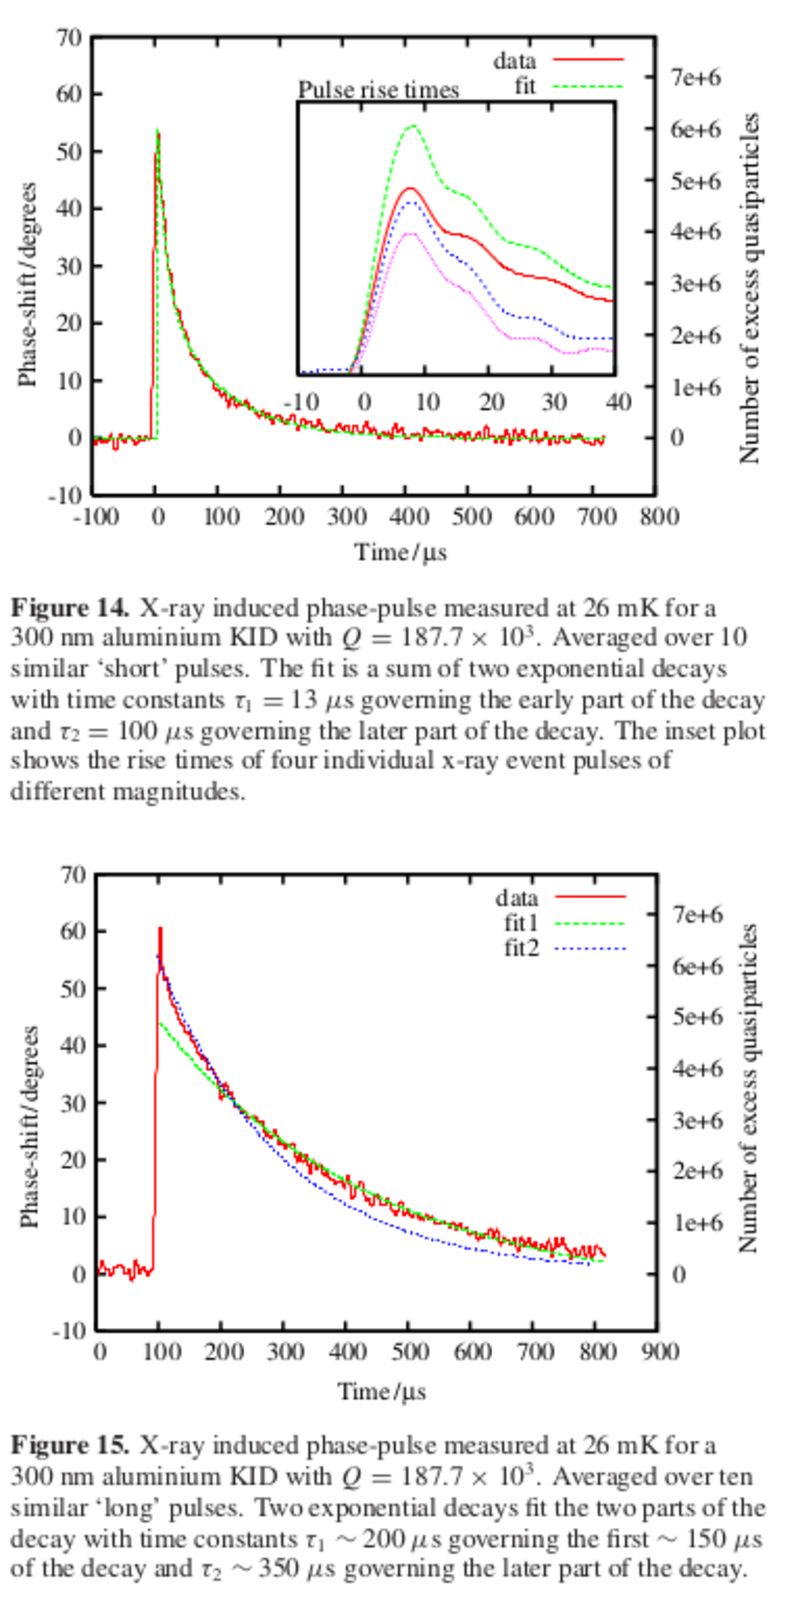
\includegraphics[width=0.62\textwidth]{pulso_respuesta_mkid}
								\end{column}
								\begin{column}{0.49\textwidth}
												\footnotesize{The KID detection mechanism $\to$ a
												temporal change in the surface kinetic inductance
												of a superconductor when a photon of energy $h\nu \geq
												2 \Delta(T)$ is absorbed, where $\Delta(T)$ is the
												superconducting gap parameter.
												\pause

												High energy photons break
												Cooper pairs. These recombine in a characteristic time,
												of the order $10-500\,\mu\text{s}$,
												{\color{red}producing pulse-like changes in the surface
												impedance}.
												\pause

												As the impedance of a superconductor is
												mostly inductive, especially for $T << T_c$, the
												superconductor can be engineered as the inductive
												element in a RLC-like resonant circuit.
												\pause

												{\color{blue}The
												quality factor of the resonant circuit determines both the
												\alert{sensitivity} and \alert{speed} of the device}.}
								\end{column}
				\end{columns}
\end{frame}
\begin{frame}{MKIDs}
				\framesubtitle{Energy resolution}
				%\begin{exampleblock}{}
				%       Works on the principle that incident photons change the surface
				%       impedance of a superconductor through the \textit{kinetic
				%       inductance effect}
				%\end{exampleblock}
												\begin{equation}
																R = \frac{1}{2.355}\sqrt{\frac{\eta h \nu}{F
																\Delta}}
												\end{equation}
				$\eta = 0.57 \to$ efficiency of creating quasiparticles,

				$h\nu \to$ energy of the incident photon,

				$\Delta = 1.72 k_BT_c \to$ gap energy of the superconducting absorber,

				$F \approx 0.2 \to$ Fano factor

				$R=150$ at 5\,eV for an operating temperature of 100\,mK.

				An operating temperature of 15\,mK could allow a theoretical
				maximum energy resolution of $R=400$ at 5\,eV (although it is likely other
				noise sources, like two level system noise, will become more important
				as future development increases the energy resolution).

\end{frame}
\begin{frame}{MKIDs}
				%\begin{exampleblock}{}
				%       Works on the principle that incident photons change the surface
				%       impedance of a superconductor through the \textit{kinetic
				%       inductance effect}
				%\end{exampleblock}
				\scriptsize{\begin{itemize}
								\item Serve as mm/submm photon detectors
								\item Resonance  $1-10\,\text{GHz}$
								\item $Q \sim 10^5$
								\item $T_{op} < 300\,\text{mK}$
								\item Intrinsic energy resolution $R = \frac{E}{\Delta E} \sim
												20-150$\footnote{Rev.Sci.Instr. 83, 044702 (2012)}
								\item The resonators are designed to be separated by 2\,MHz
												within a $4-5\,\text{GHz}$ band.
								\item Off-resonance transmission $\simeq 1$
												%       \begin{equation}
												%               R = \frac{1}{2.355}\sqrt{\frac{\eta h \nu}{F
												%               \Delta}}
												%       \end{equation}
				\end{itemize}
				Each resonator will have a $BW \sim 200\,\text{kHz}$ (\alert{based on the
				quality factor we need}), 

				2\,MHz separation between the resonators is required (resonator position
				will move around based on different loading. If we pack them too close
				to each other, their relative position might change during observation
				or from different fridge cook down cycle).

				So we want to have ADC to have BW at least 400\,MHz, and has SNR greater
				than 59\,dB. 

				If we just consider quantization noise, theoretically, 59\,dB SNR will
				require ADC to have at least 10 bits
				}
				+----  7 lines: , but in real world, we can only find 10 bits ADC------------------------------------------------------------------------------------------------------------
				\tiny{\textbf{arXiv:1310.5891v2 (2013)}}
\end{frame}
\begin{frame}{MKID}
				\begin{itemize}
								\item Los MKID funcionan según el principio de que los fotones
												incidentes \alert{cambian la impedancia de la superficie de un
												superconductor a través del efecto de inductancia
												cinética} (Mattis y Bardeen, 1958).
								\item 
								\item ¿Qué beneficios obtengo/obtenemos?
								\item ¿Qué grupos integro/se formaron con esto?
								\item 
								\item 
				\end{itemize}

\end{frame}

\begin{frame}{Tipos de MKIDs}
				\begin{itemize}
								\item OLE Doyle et.al 2008
								\item ¿Por qué lo hago?
								\item ¿Qué beneficios obtengo/obtenemos?
								\item ¿Qué grupos integro/se formaron con esto?
								\item 
								\item 
				\end{itemize}

\end{frame}

%------------------------------------------------------------------------------
\section{ARCONS}
\begin{frame}{ARCONS}

				\textbf{A}rray \textbf{C}amera for \textbf{O}ptical to \textbf{N}ear-IR
				\textbf{S}pectrophotometry
				\begin{itemize}
								\item Primer instrumento terrestre basado en MKIDs para el rango de
												longitud de onda óptica hasta el IR cercano
								\item Diseño óptico simple que permite muy alto rendimiento
								\item Resolución de tiempo de hasta seis órdenes de magnitud
												mejor que un CCD
								\item Ancho de banda intrínseco extremadamente amplio (0.1
												-5\,$\mu$m) con buena eficiencia cuántica
								\item Sin ruido de lectura o corriente oscura, y casi perfecto
												rechazo de rayos cósmicos
								\item No se pierde tiempo de observación al leer la matriz
				\end{itemize}

				%\begin{center}
				%				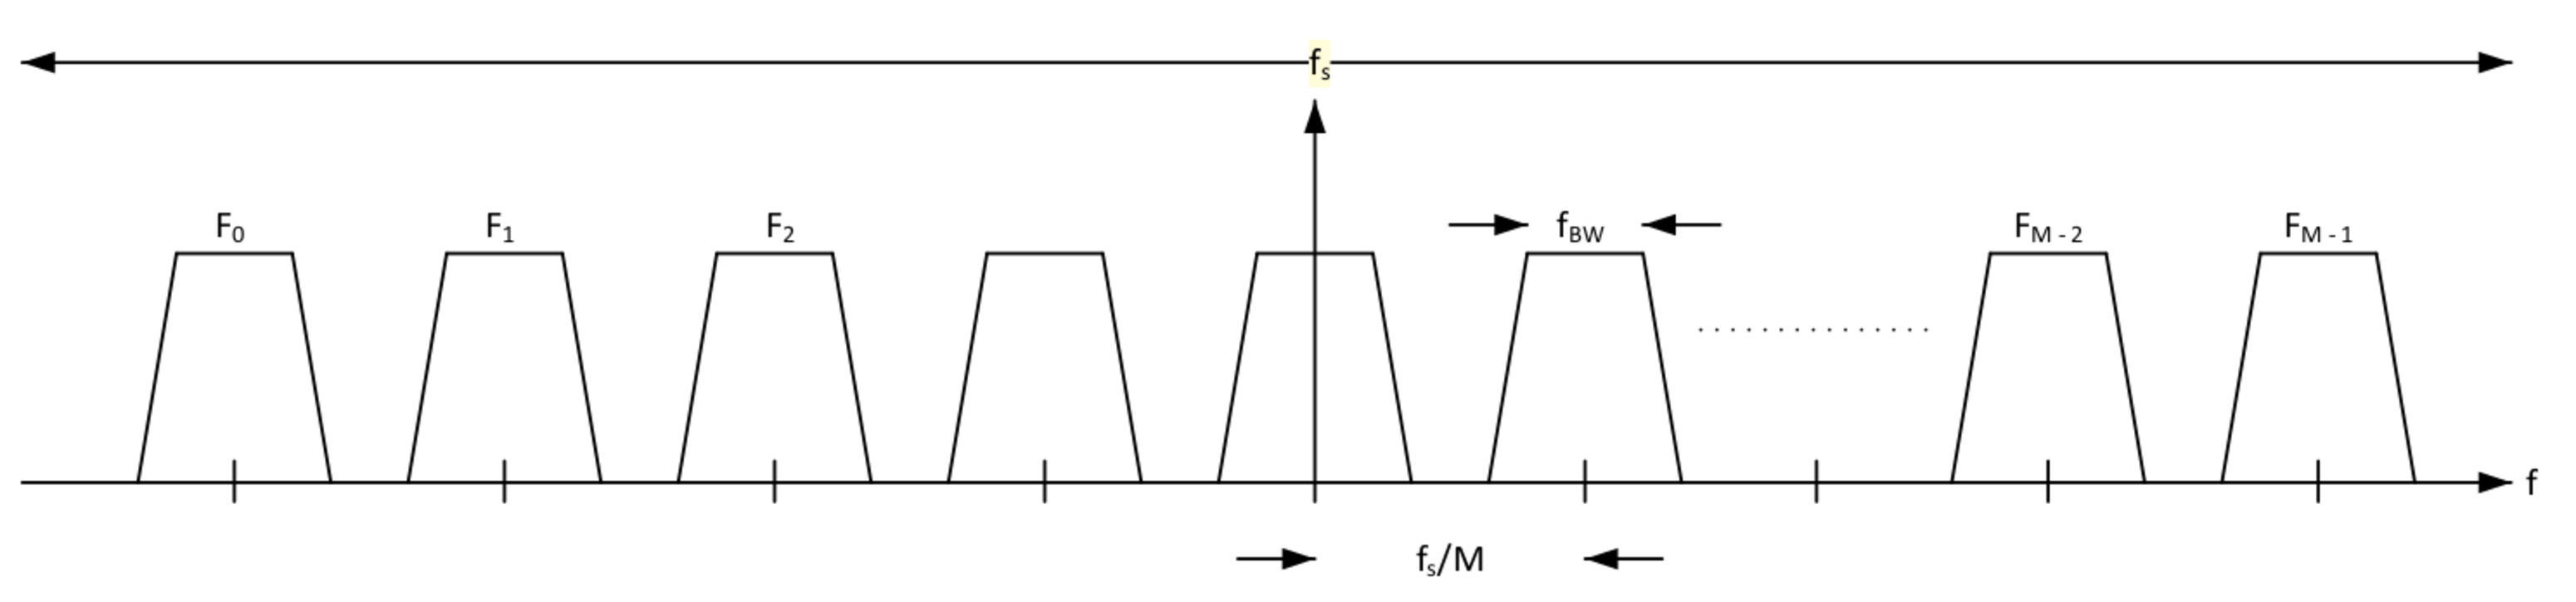
\includegraphics[width=0.8\textwidth]{FDM_channel_diagram}
				%\end{center}
\end{frame}
\begin{frame}{ARCONS}

				\textbf{A}rray \textbf{C}amera for \textbf{O}ptical to \textbf{N}ear-IR
				\textbf{S}pectrophotometry
				\begin{itemize}
								\item La tecnología actual óptica MKID tiene una resolución
												espectral $R = \lambda/\Delta \lambda \sim 10$ a
												\SI{4000}{\angstrom}
								\item 
								\item Resolución de tiempo de hasta seis órdenes de magnitud
												mejor que un CCD
								\item Ancho de banda intrínseco extremadamente amplio (0.1
												-5\,$\mu$m) con buena eficiencia cuántica
								\item Sin ruido de lectura o corriente oscura, y casi perfecto
												rechazo de rayos cósmicos
								\item No se pierde tiempo de observación al leer la matriz
				\end{itemize}

				%\begin{center}
				%				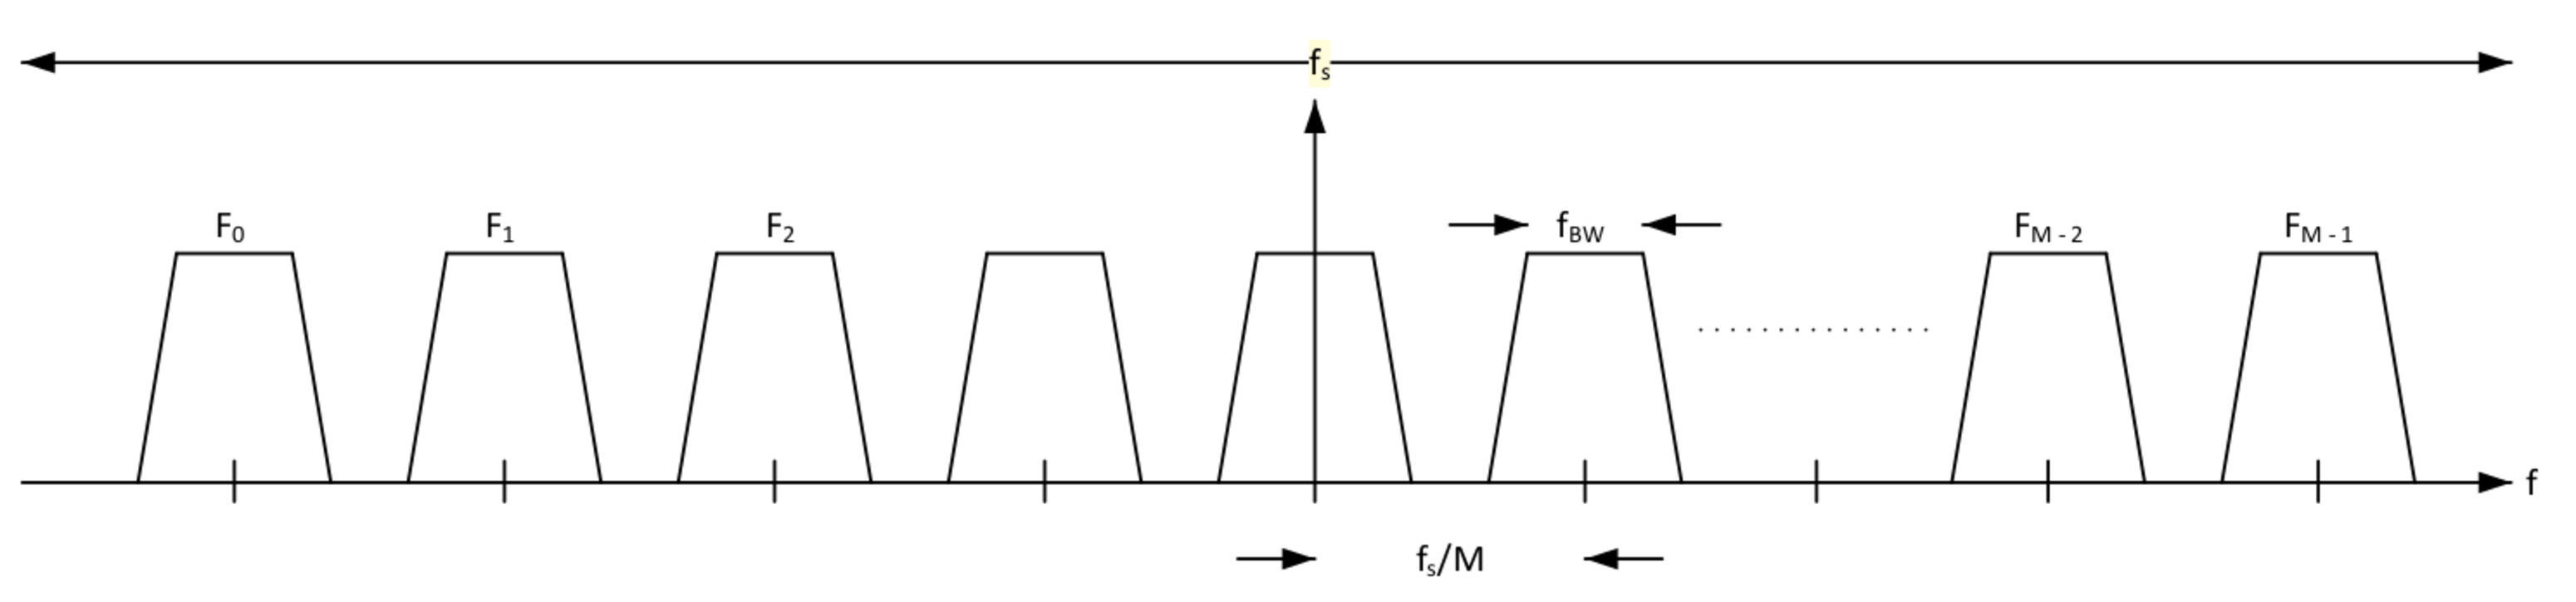
\includegraphics[width=0.8\textwidth]{FDM_channel_diagram}
				%\end{center}
\end{frame}

%------------------------------------------------------------------------------
\section{Channelizer}
\begin{frame}{Canalizador (Channelizer)}

				Implementación m\'as eficiente en t\'erminos de uso de hardware en FPGA

				Ancho de banda similar para todos los canales 

				Extensible a un n\'umero grande de canales ($>=1000$)

				Posibilidad de realizar el diseño en multi-etapas

				\begin{center}
								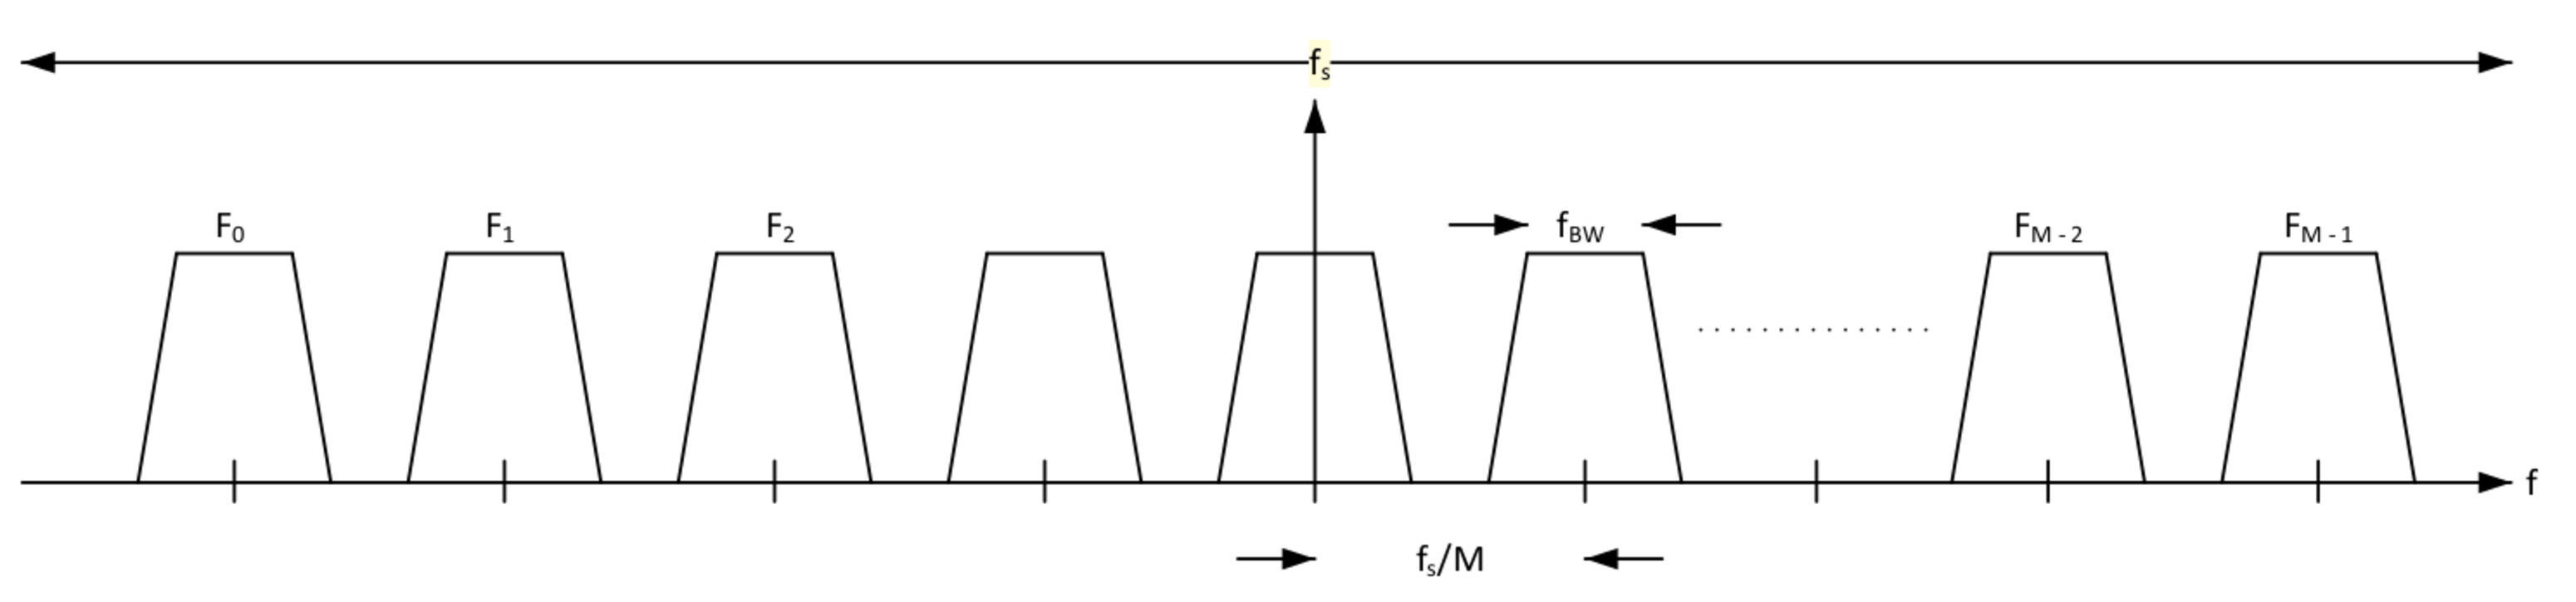
\includegraphics[width=0.8\textwidth]{FDM_channel_diagram}
				\end{center}
\end{frame}
\begin{frame}{Channelizer Tx}
				%\begin{columns}
				%				\begin{column}{0.65\textwidth}
				\begin{center}
								\only<1>{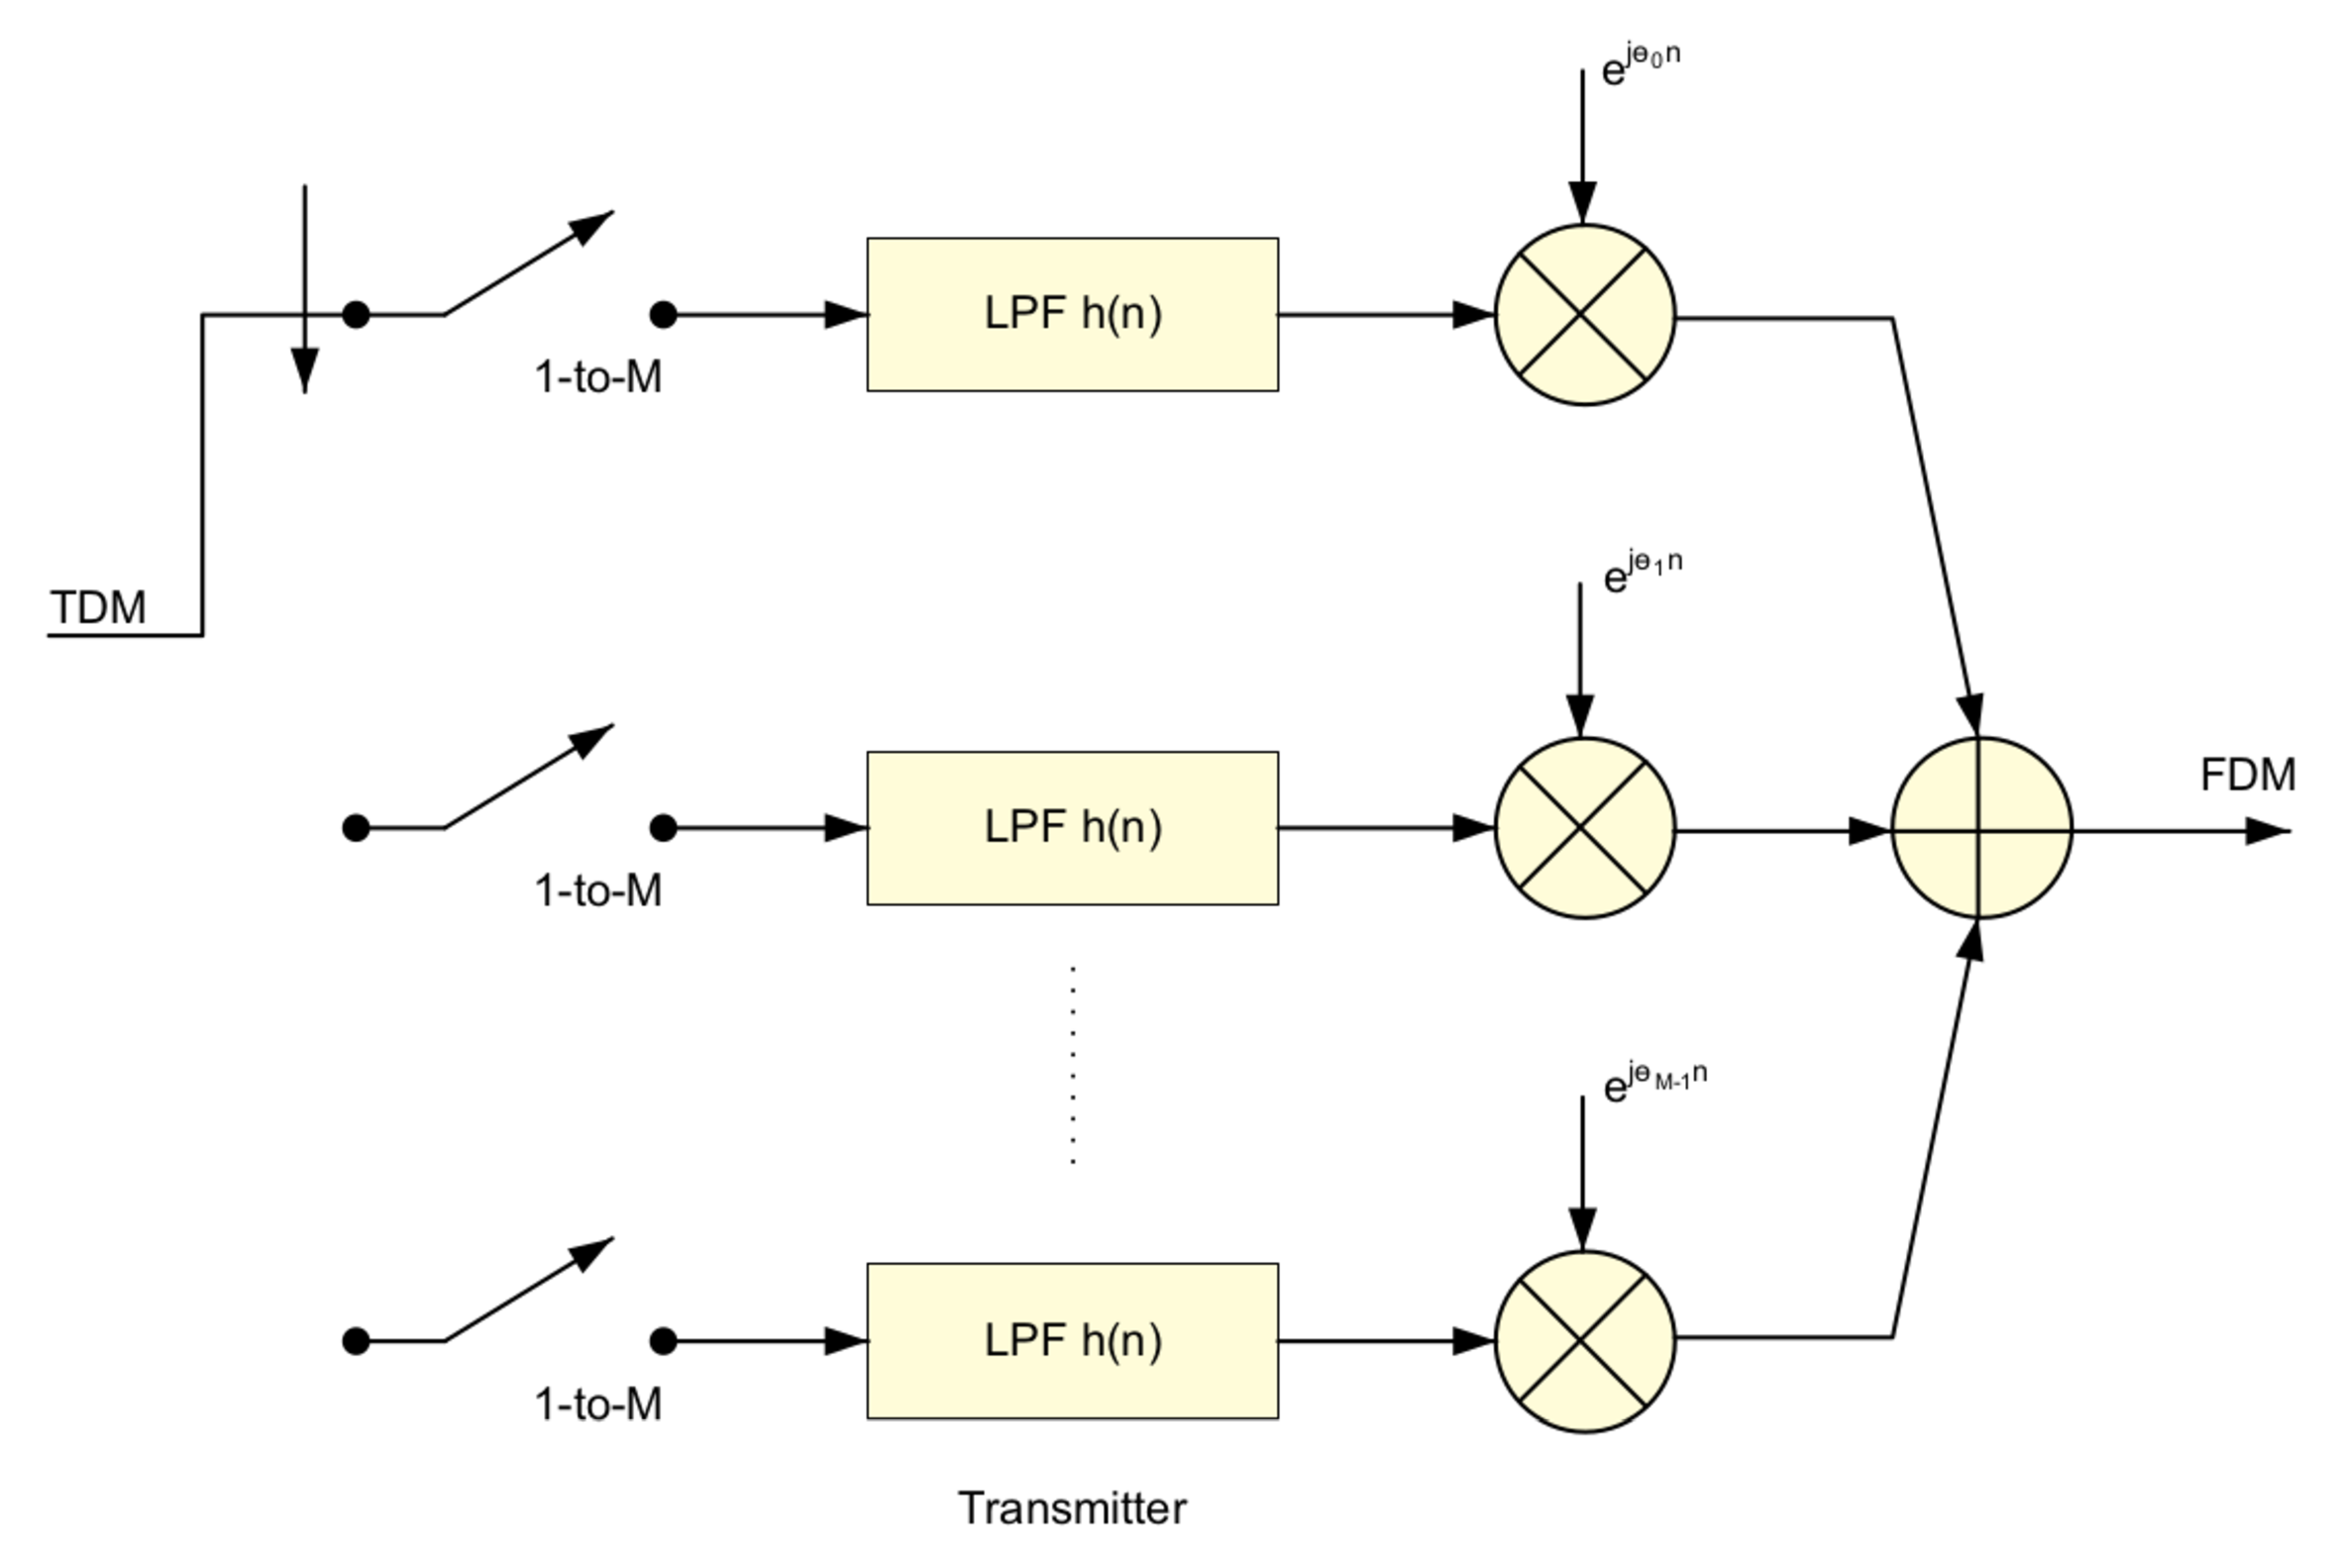
\includegraphics[width=0.8\textwidth]{Tx_channelizer}}
				\end{center}
				%				\end{column}
				%				\begin{column}{0.65\textwidth}
								\begin{center}
												\only<2>{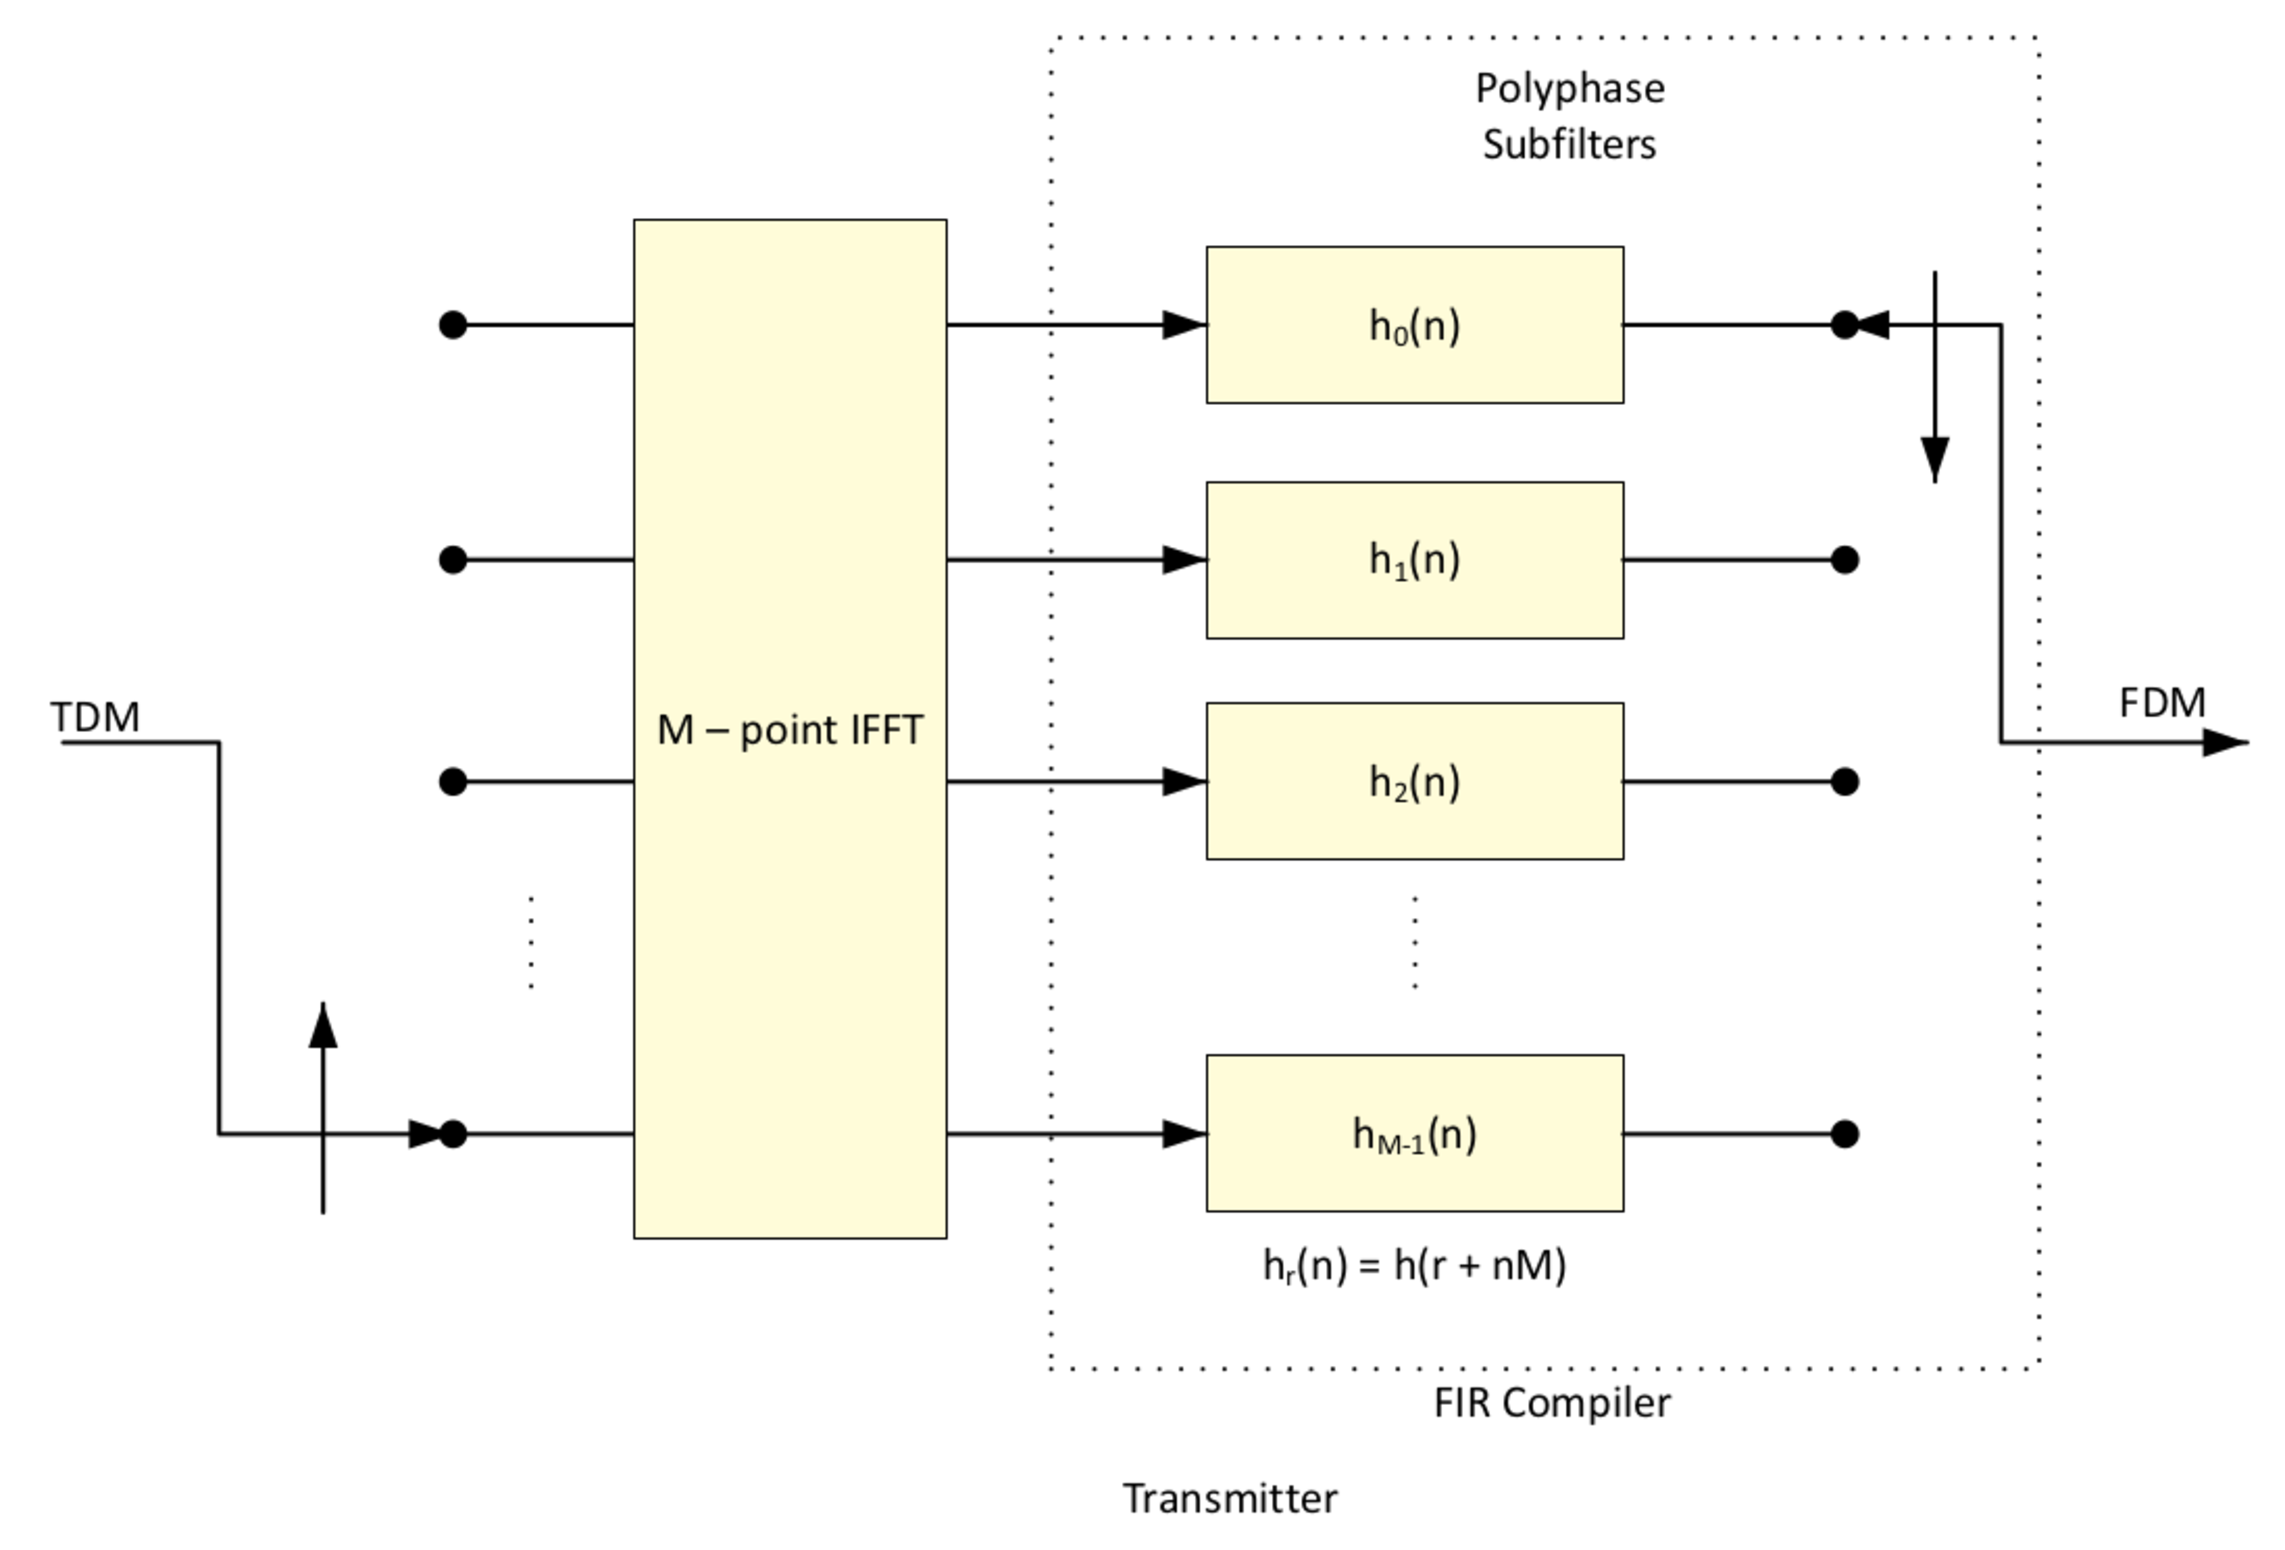
\includegraphics[width=0.8\textwidth]{Tx_channelizer_con_IFFT}}
								\end{center}
								%				\end{column}
								%\end{columns}
\end{frame}
\begin{frame}{Channelizer Rx}
				%\begin{columns}
				%				\begin{column}{0.65\textwidth}
				\begin{center}
								\only<1>{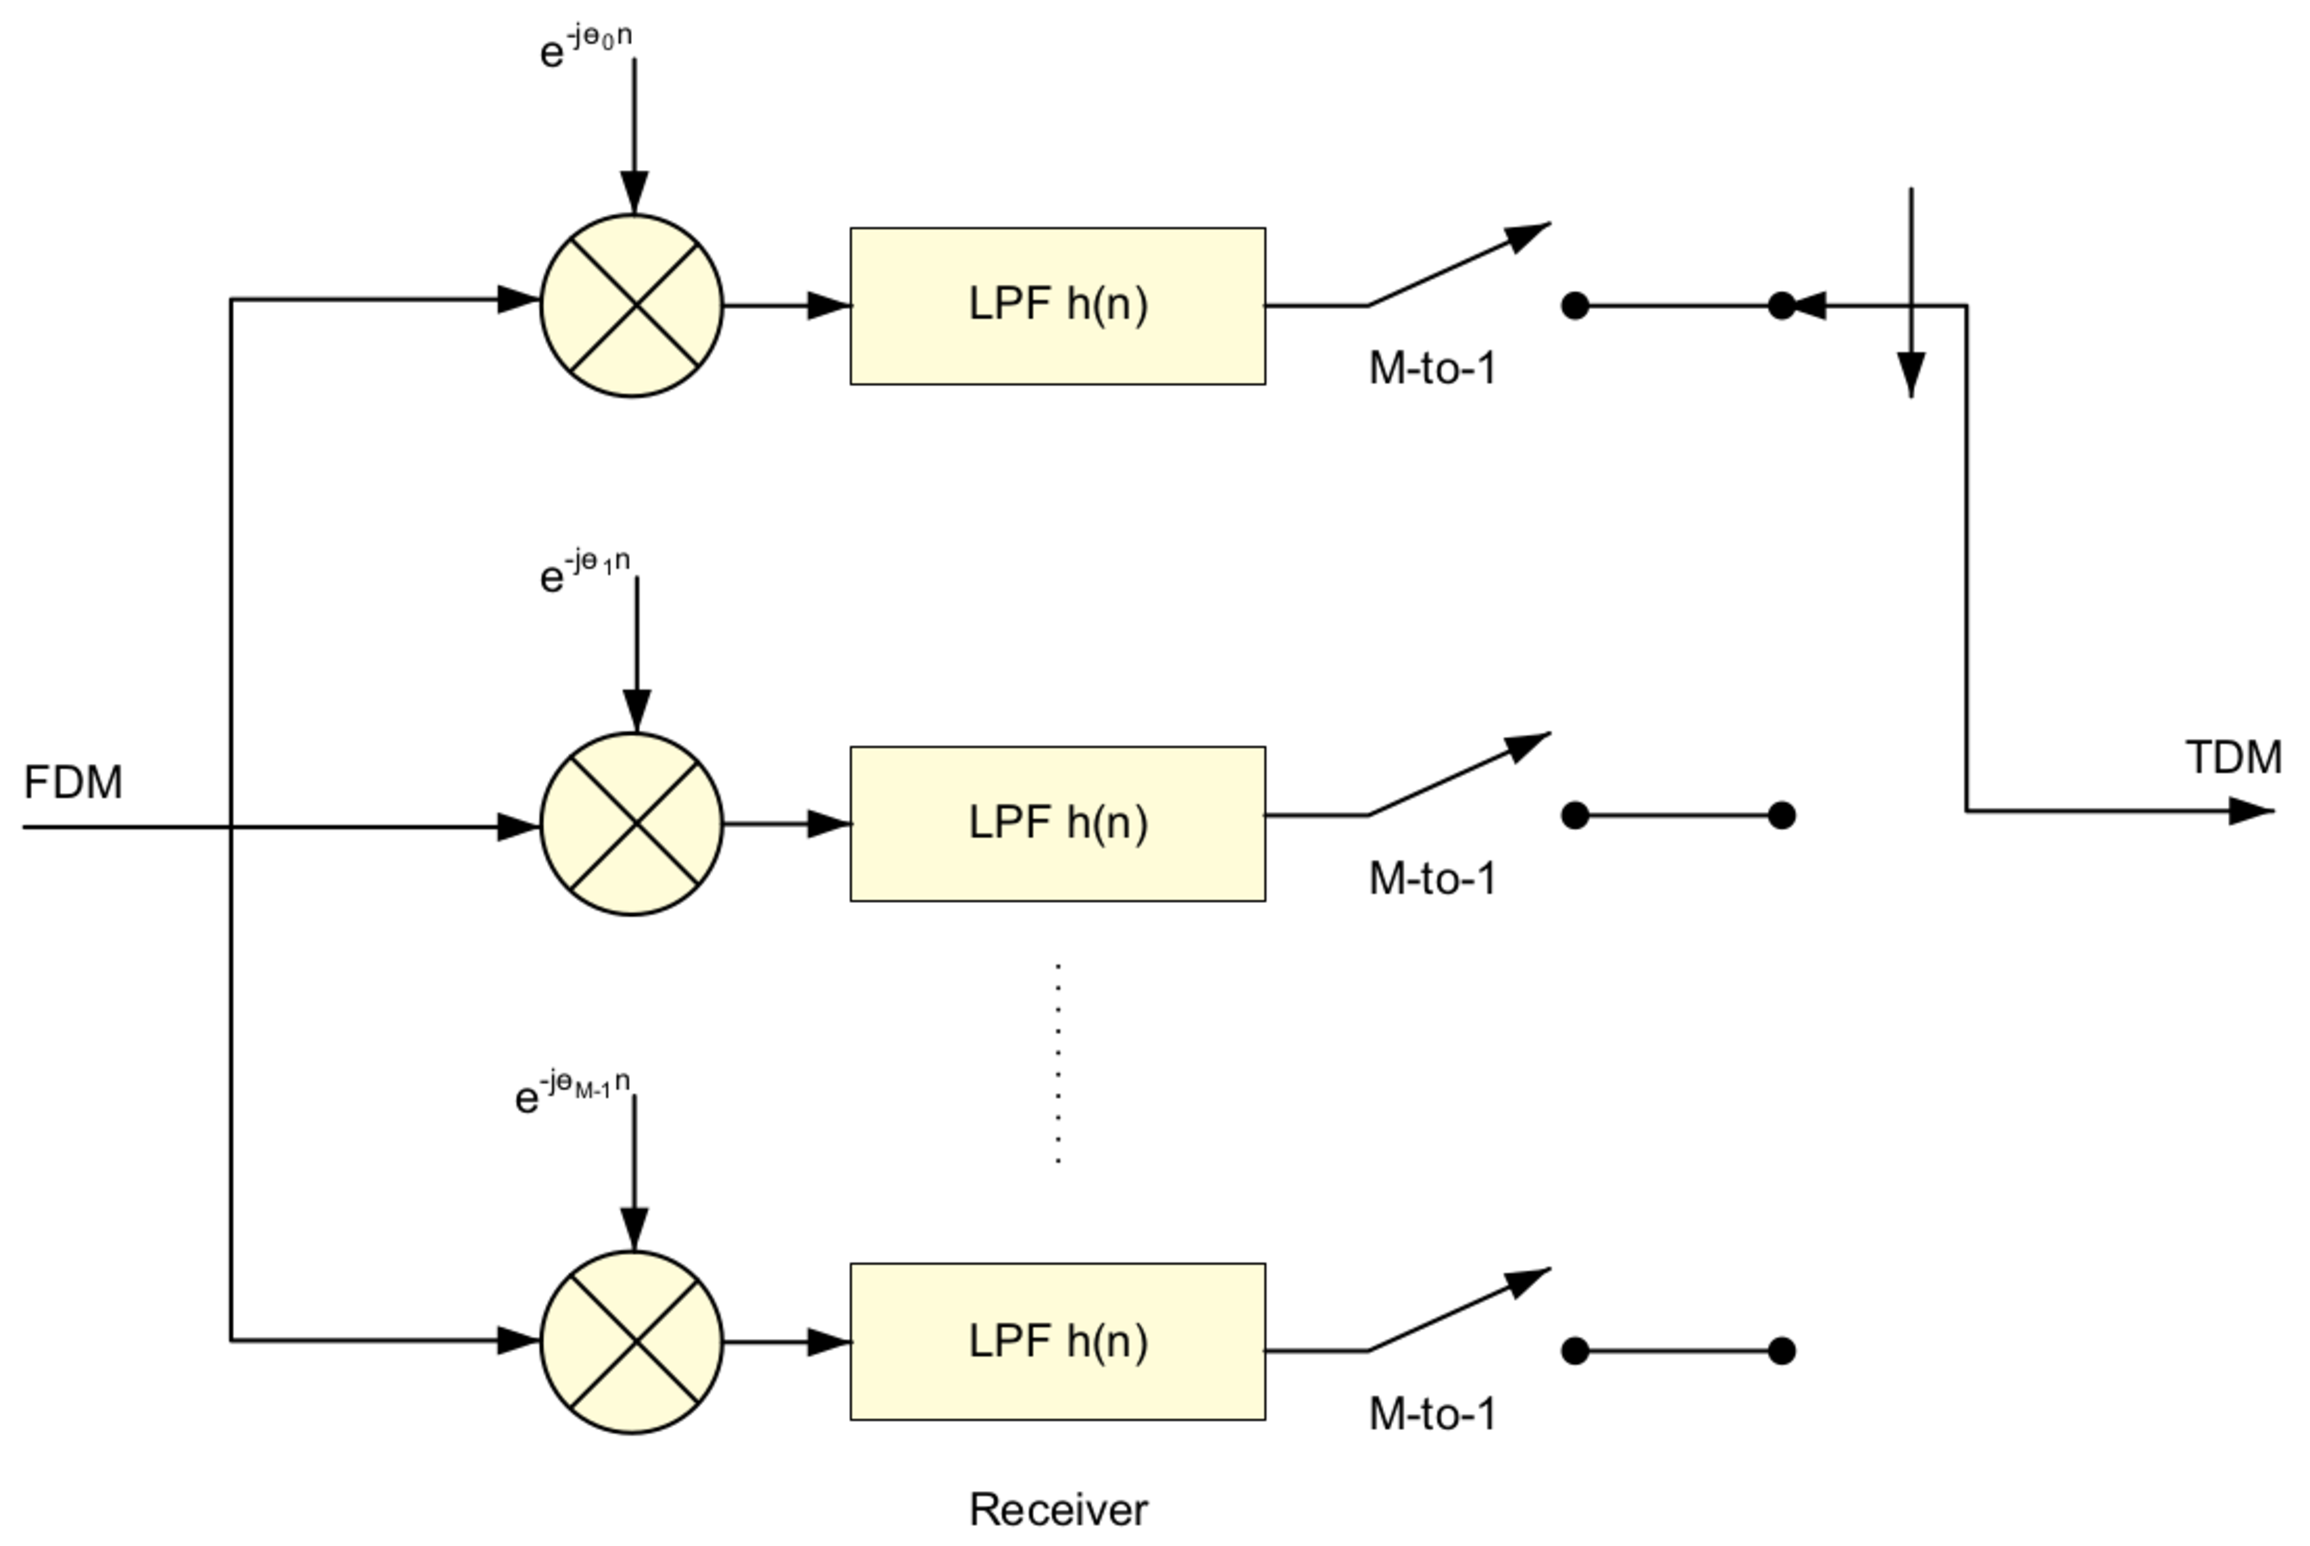
\includegraphics[width=0.8\textwidth]{Rx_channelizer}}
				\end{center}
				%				\end{column}
				%				\begin{column}{0.65\textwidth}
								\begin{center}
												\only<2>{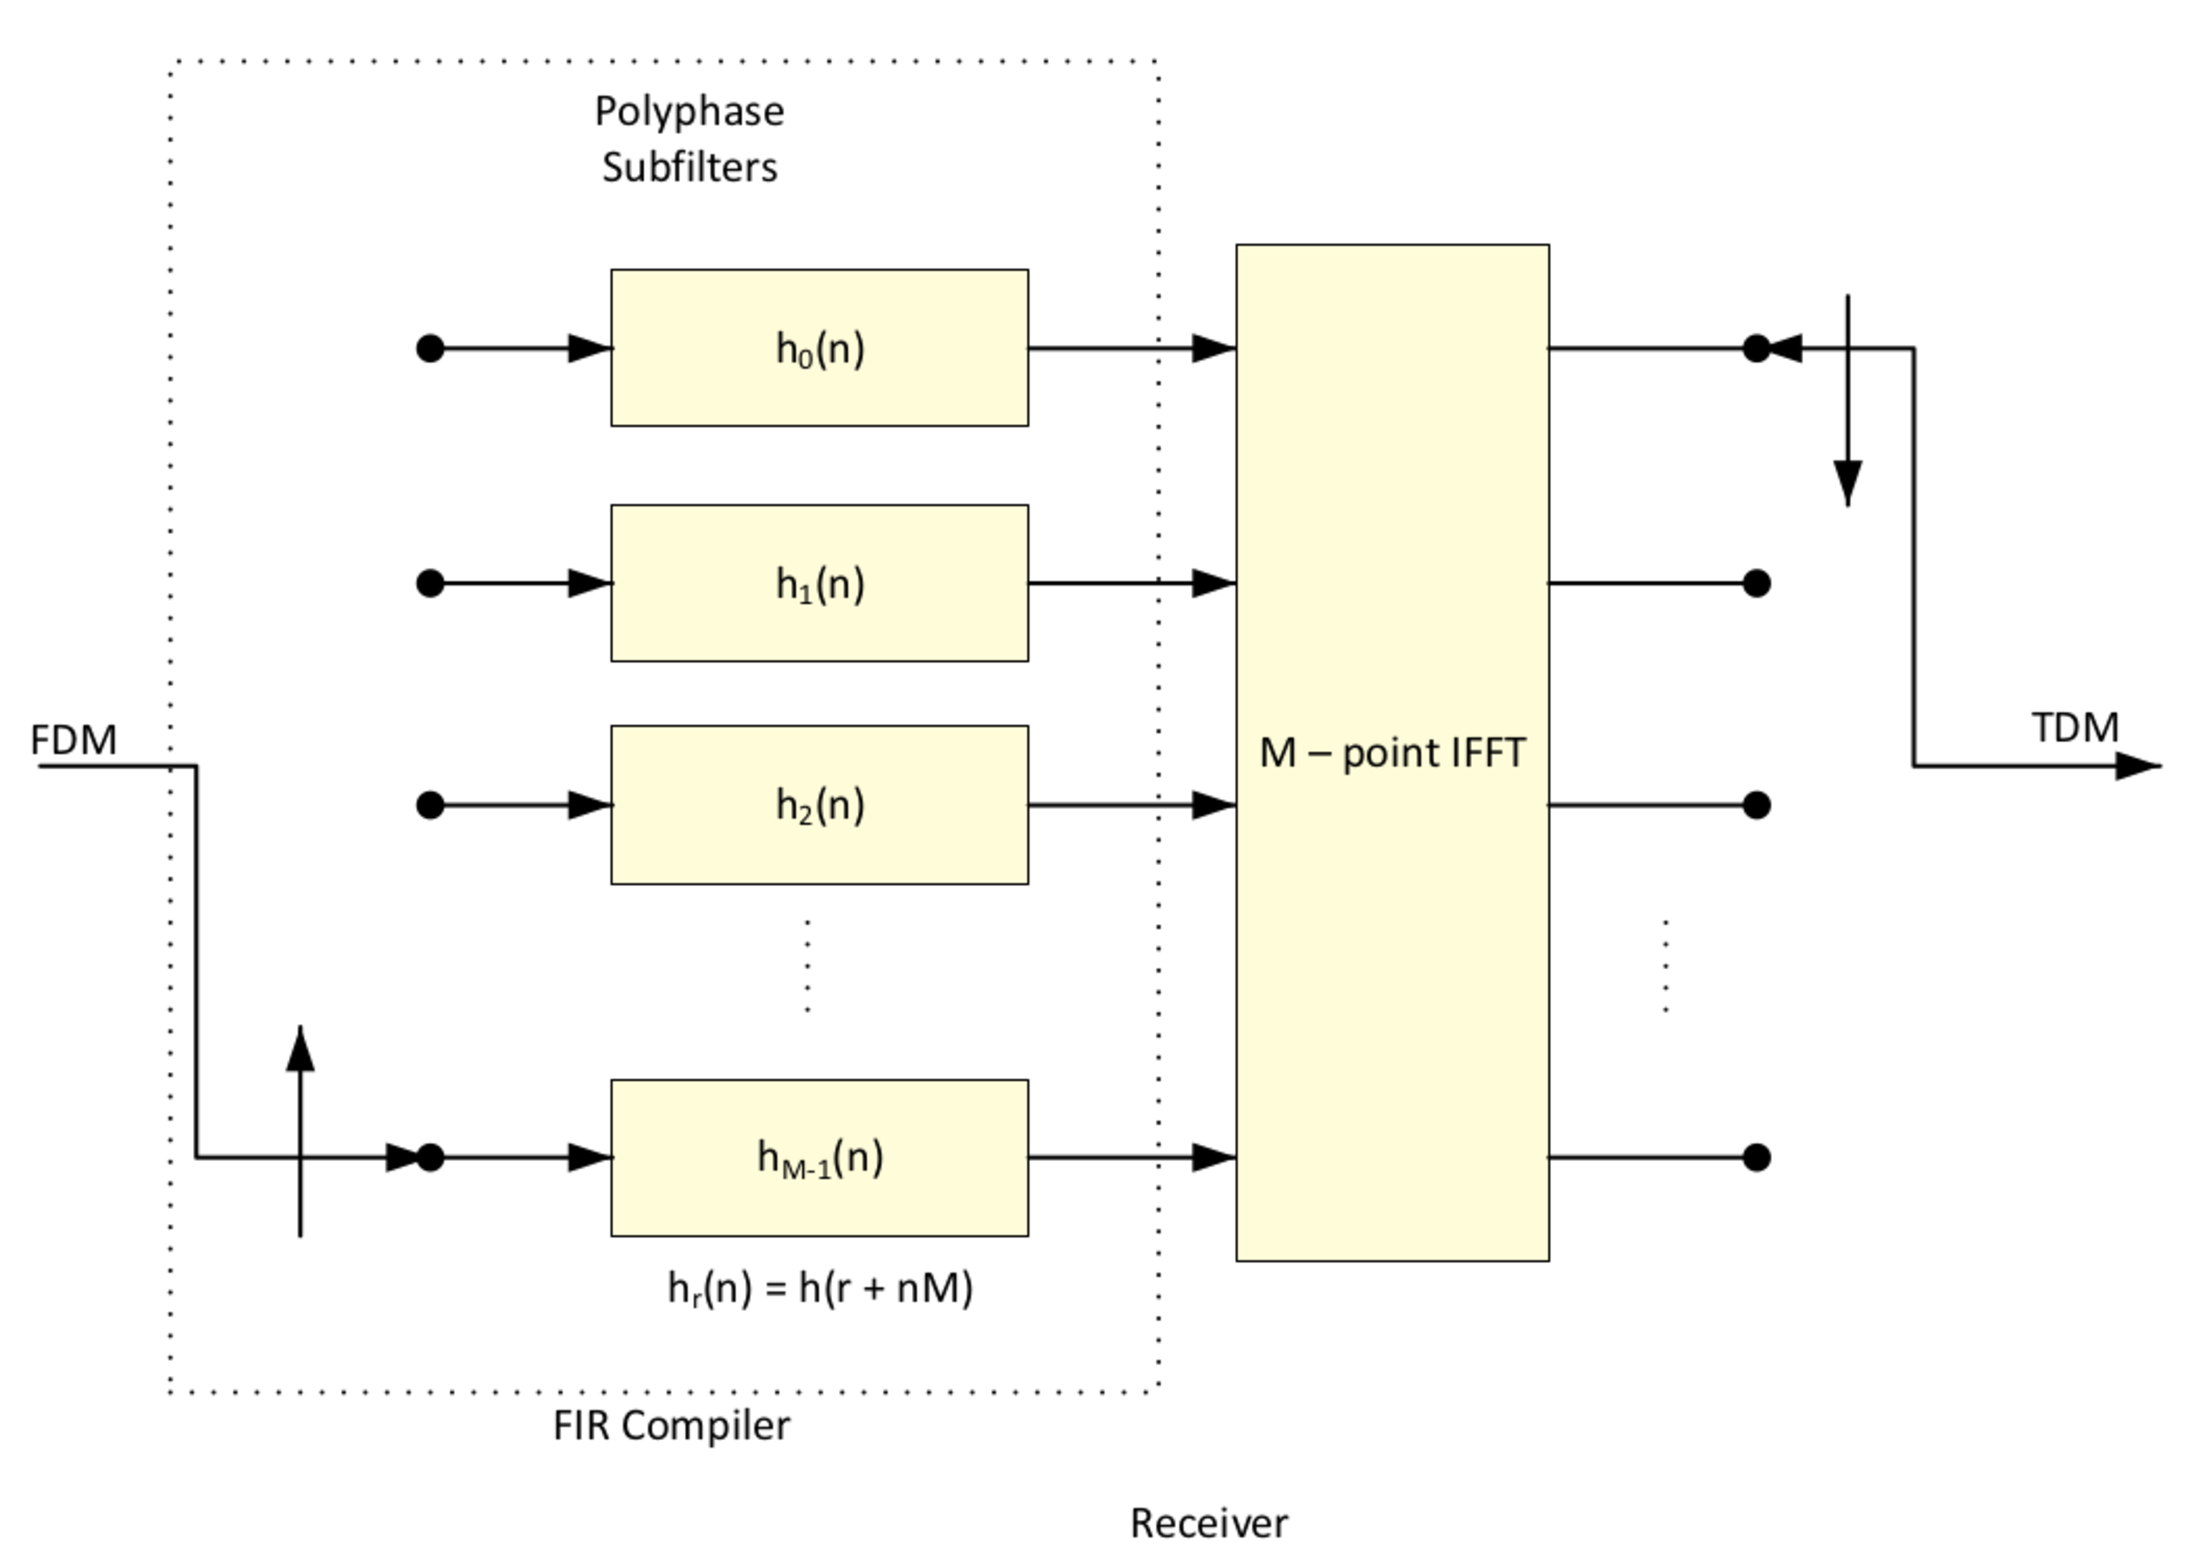
\includegraphics[width=0.8\textwidth]{Rx_channelizer_con_IFFT}}
								\end{center}
								%				\end{column}
								%\end{columns}
\end{frame}
\begin{frame}{Channelizer operación básica}
				\begin{center}
								\only<1>{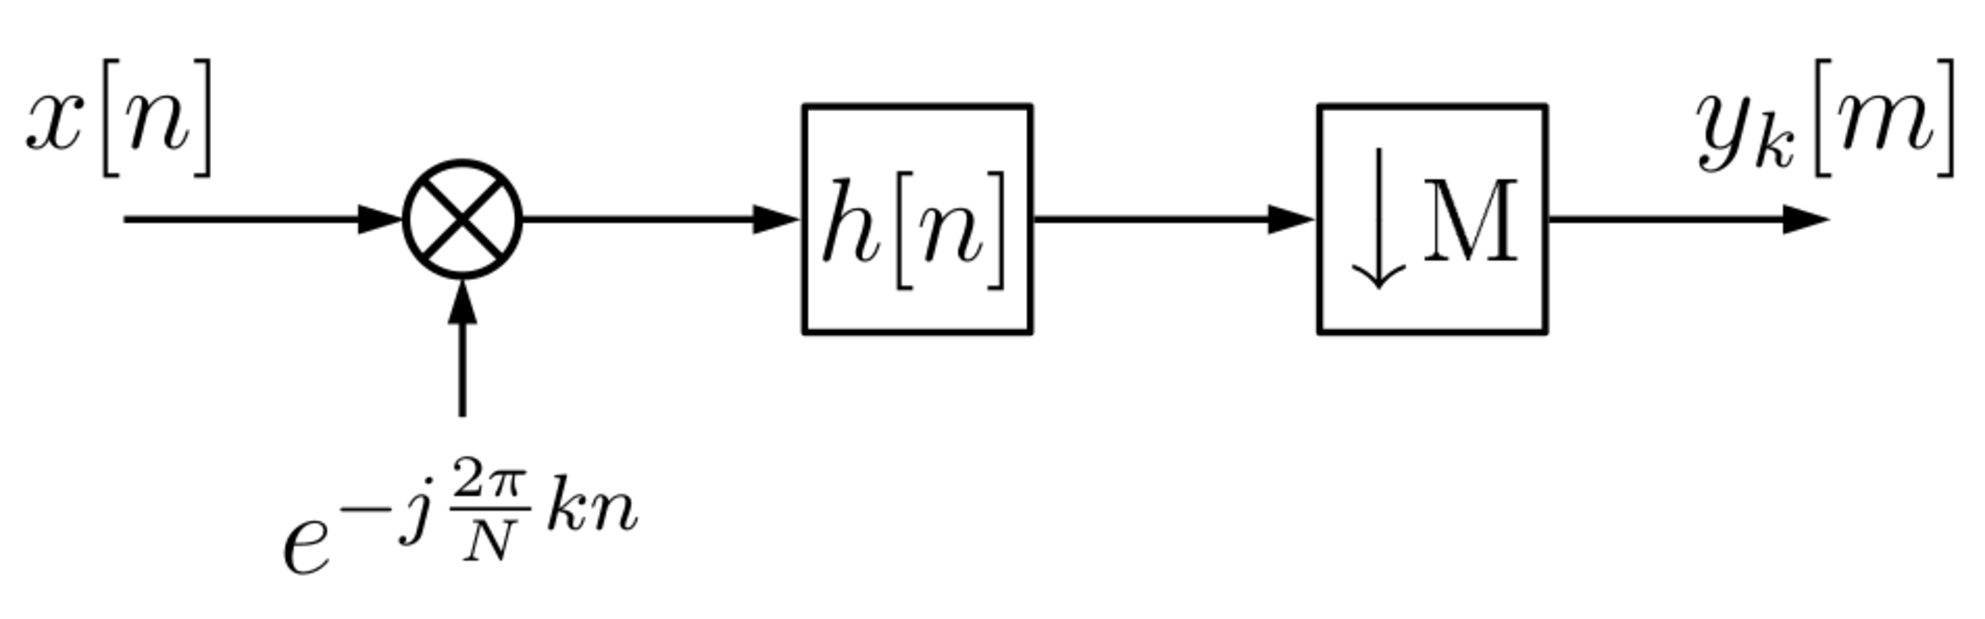
\includegraphics[width=0.8\textwidth]{PFB_basic_operation}}
				\end{center}
								\begin{center}
												\only<2>{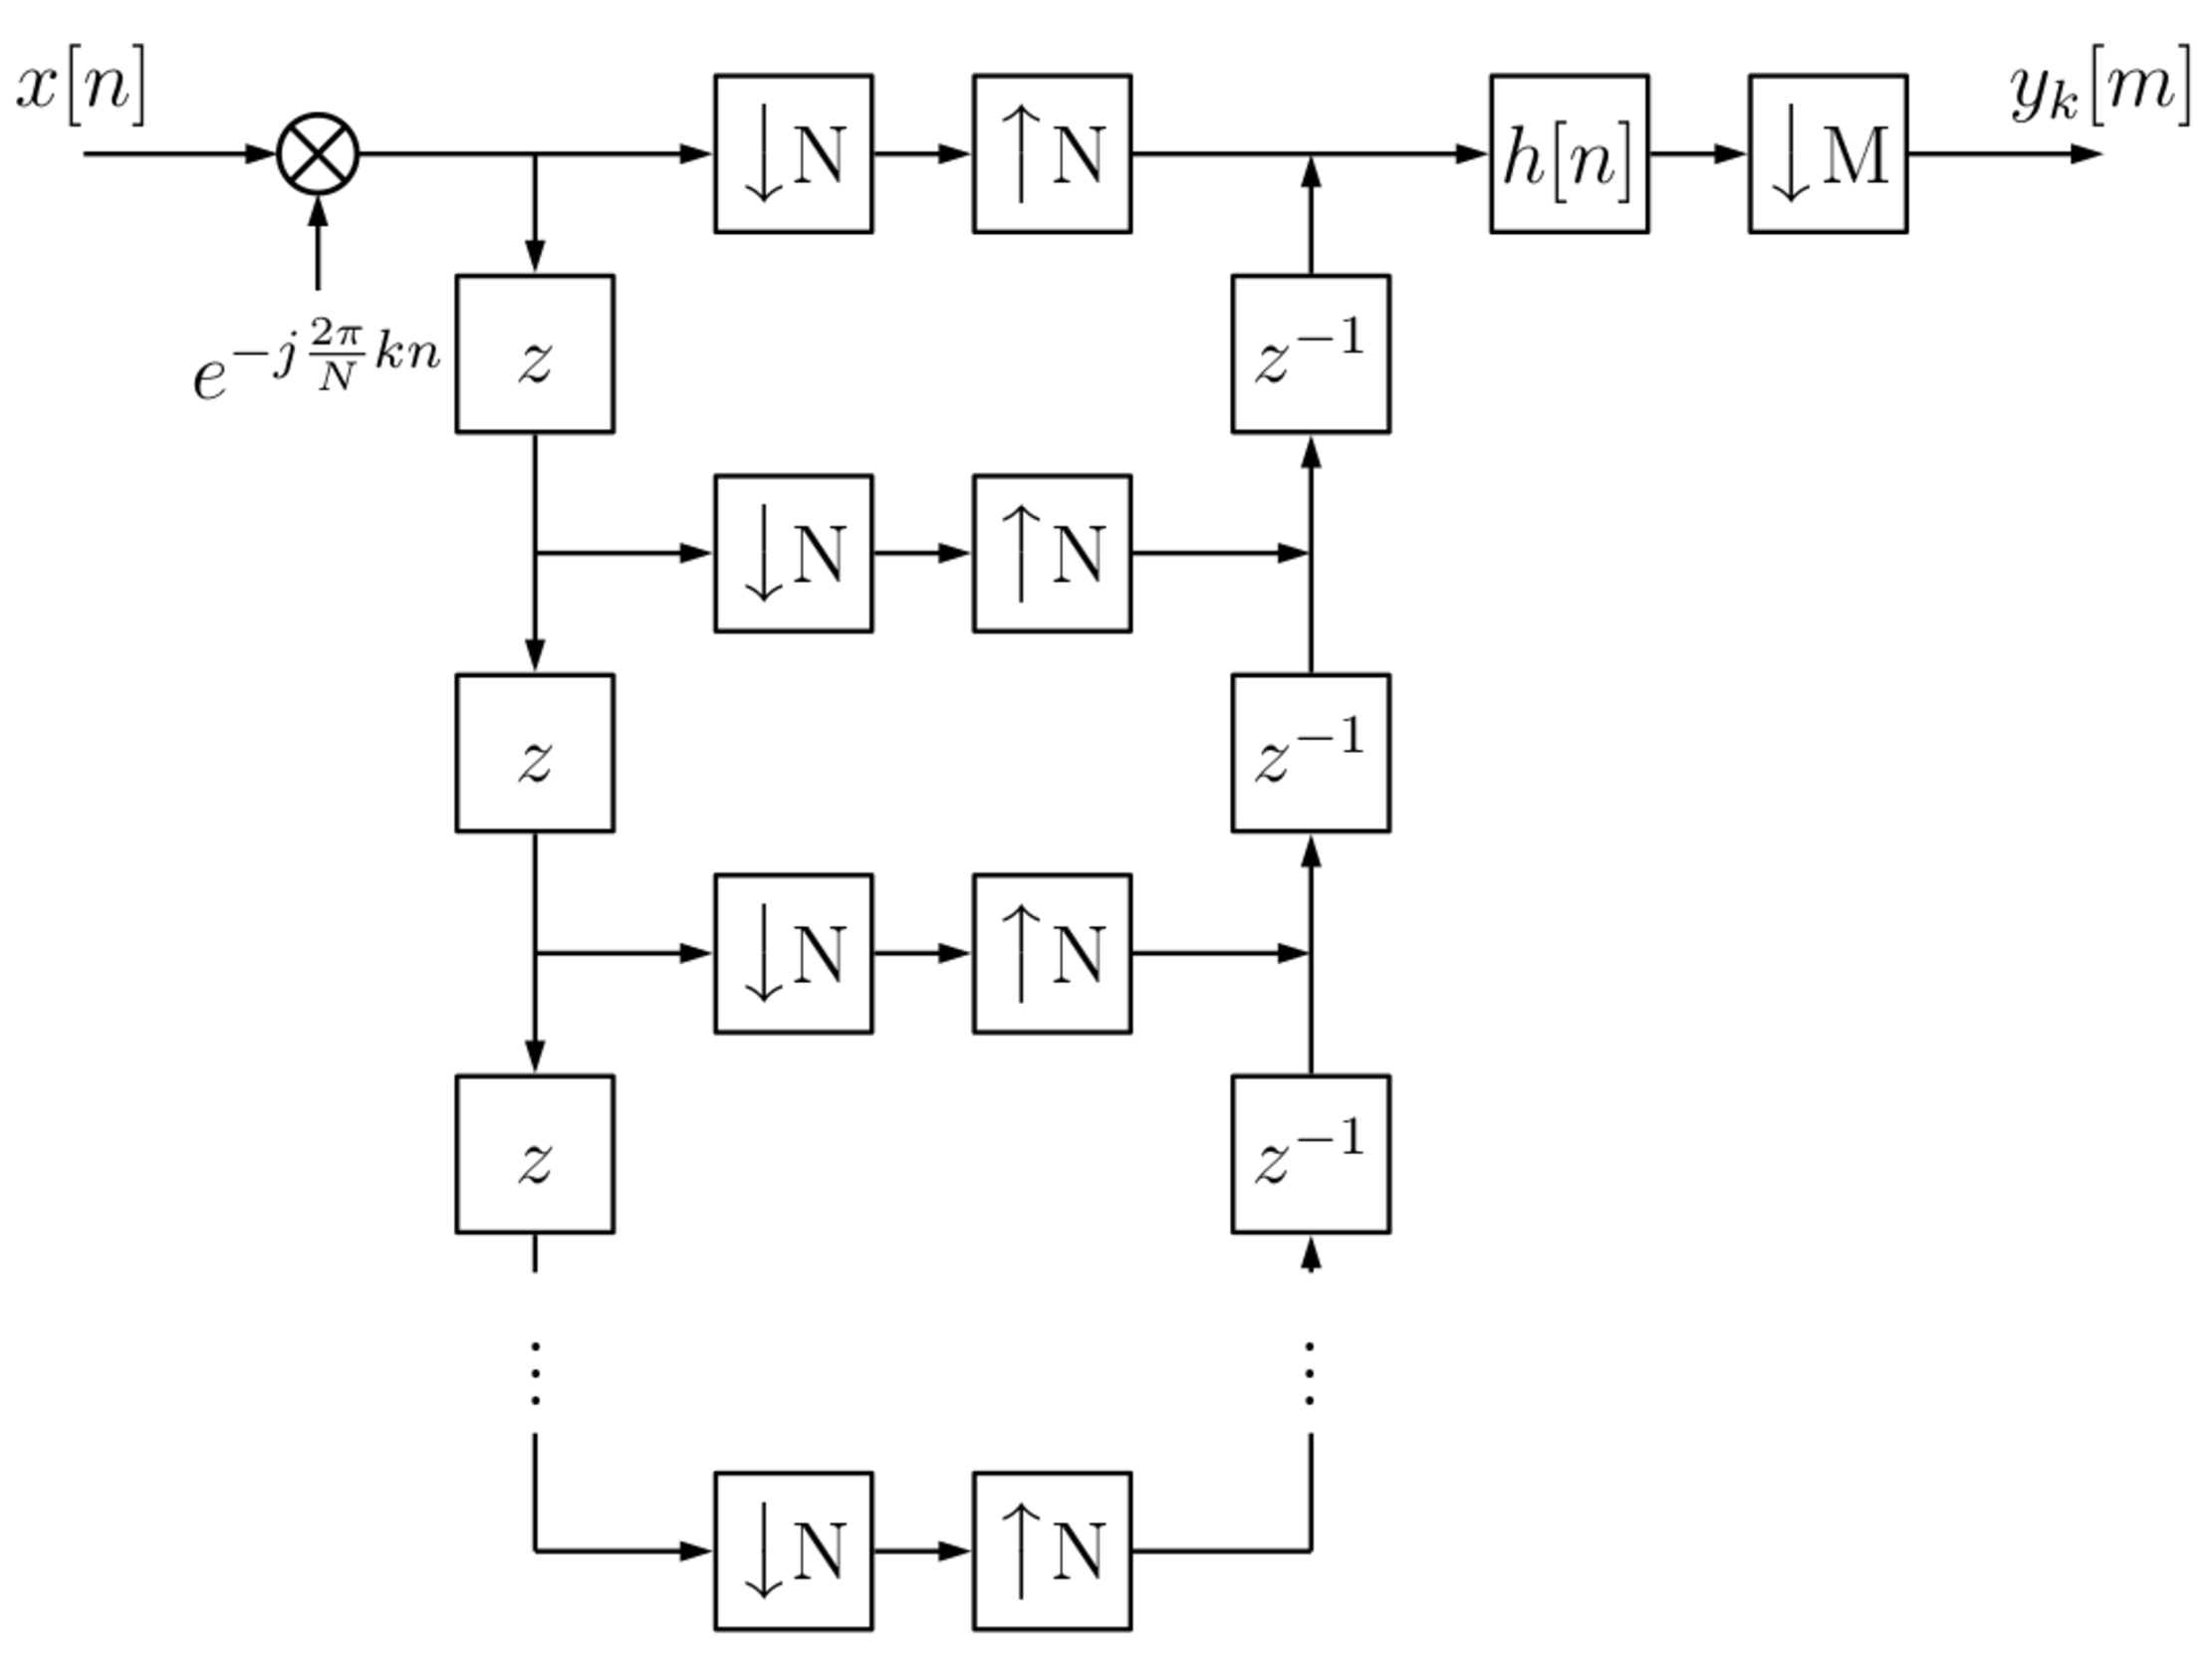
\includegraphics[width=0.8\textwidth]{PFB_opening_after_modulation}}
								\end{center}
\end{frame}
\begin{frame}{Channelizer operación básica}
				\begin{center}
								\only<1>{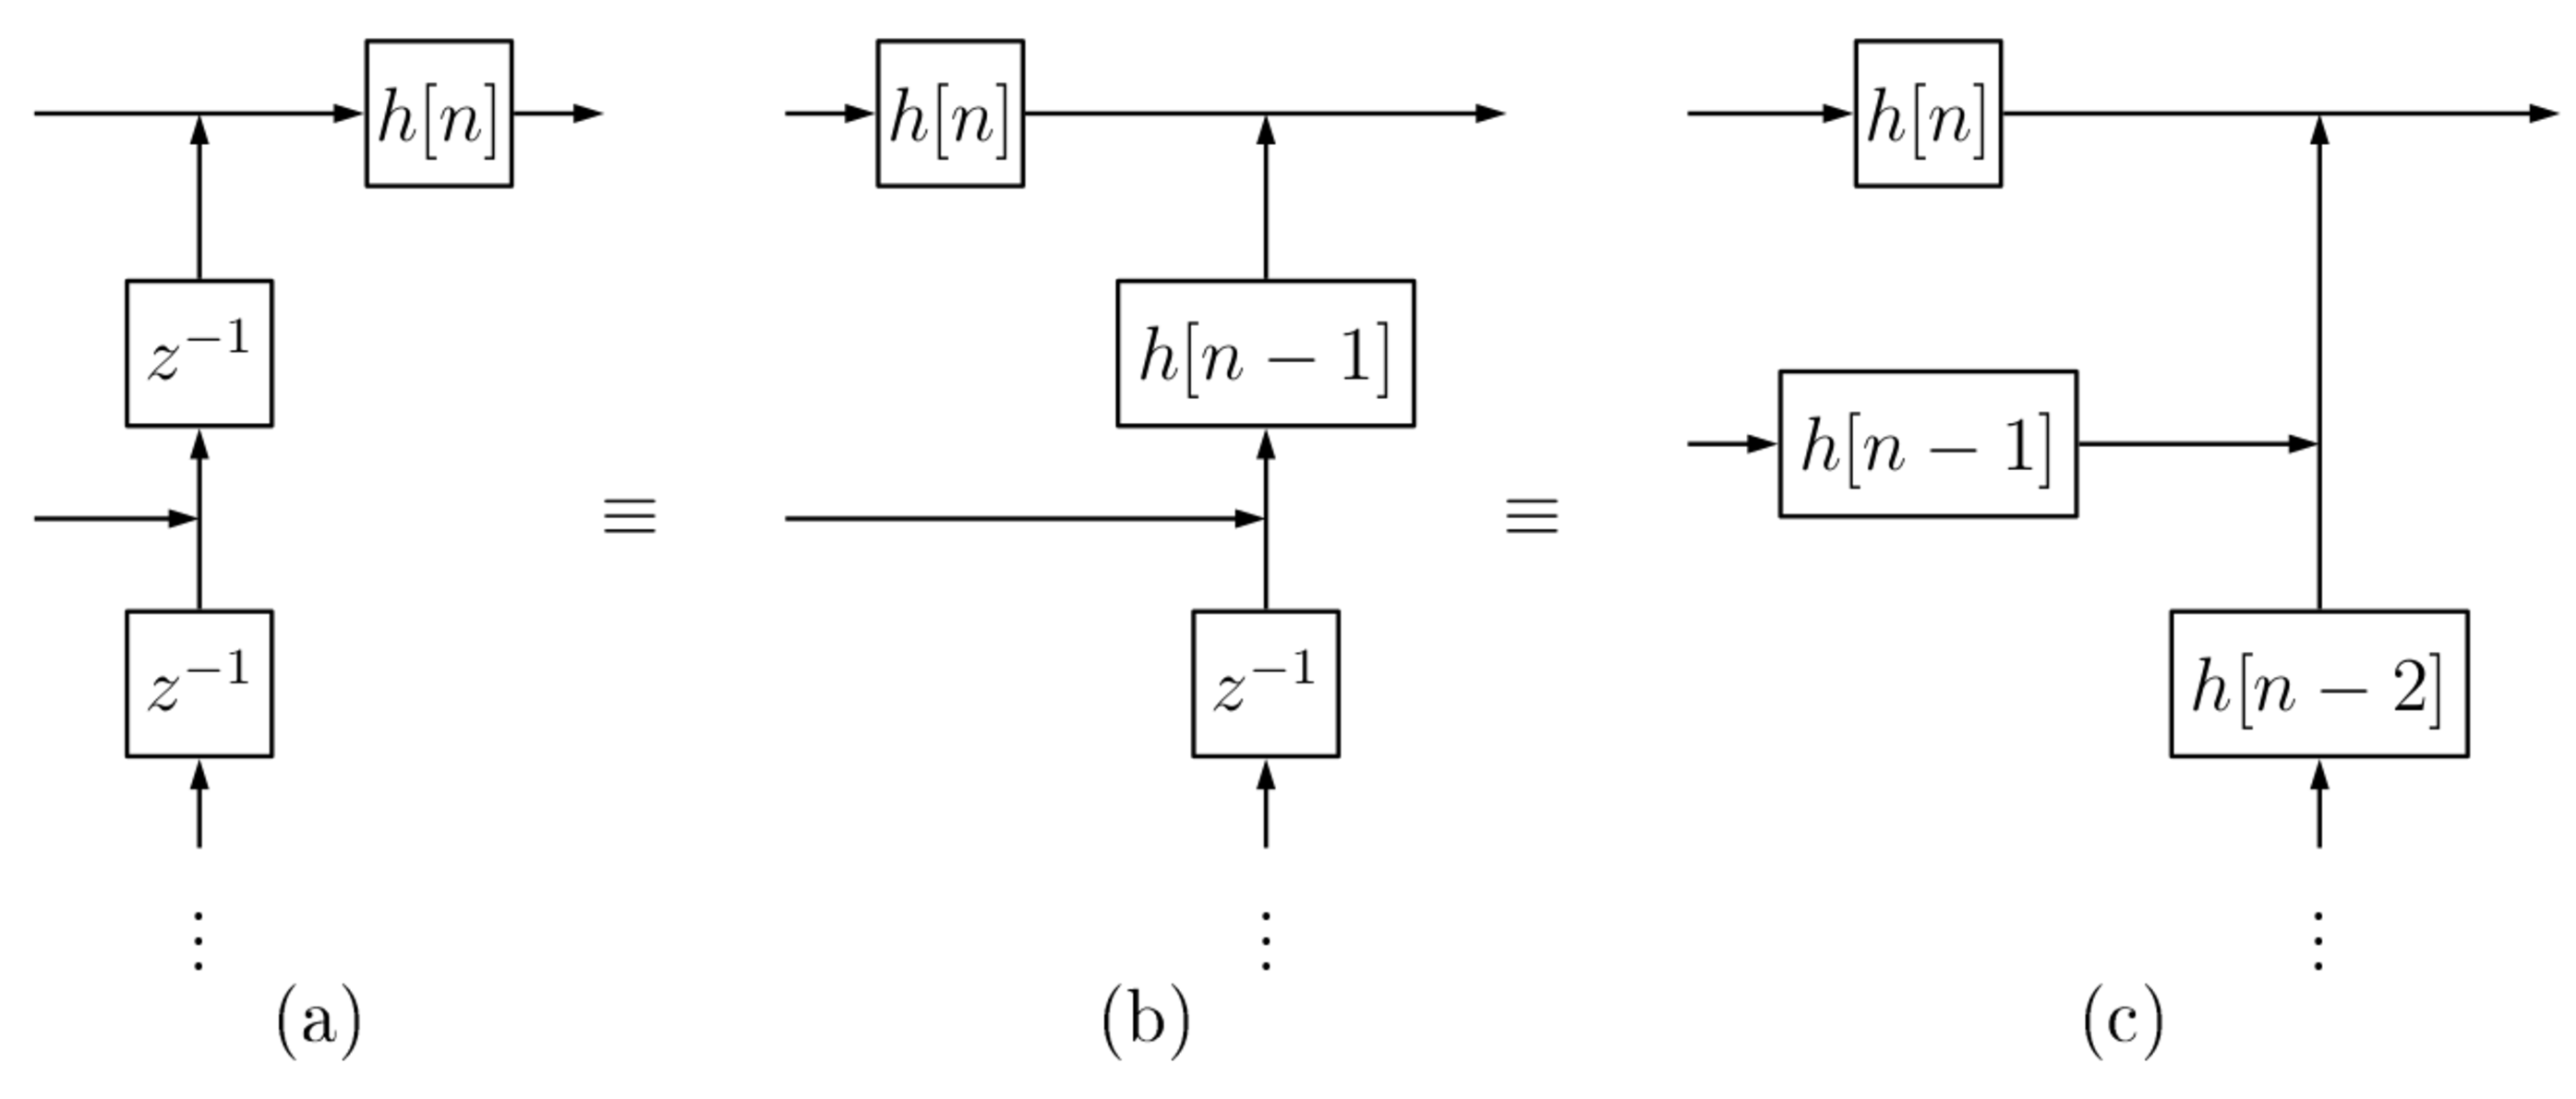
\includegraphics[width=0.8\textwidth]{PFB_distribution_filter_branches}}
				\end{center}
								\begin{center}
												\only<2>{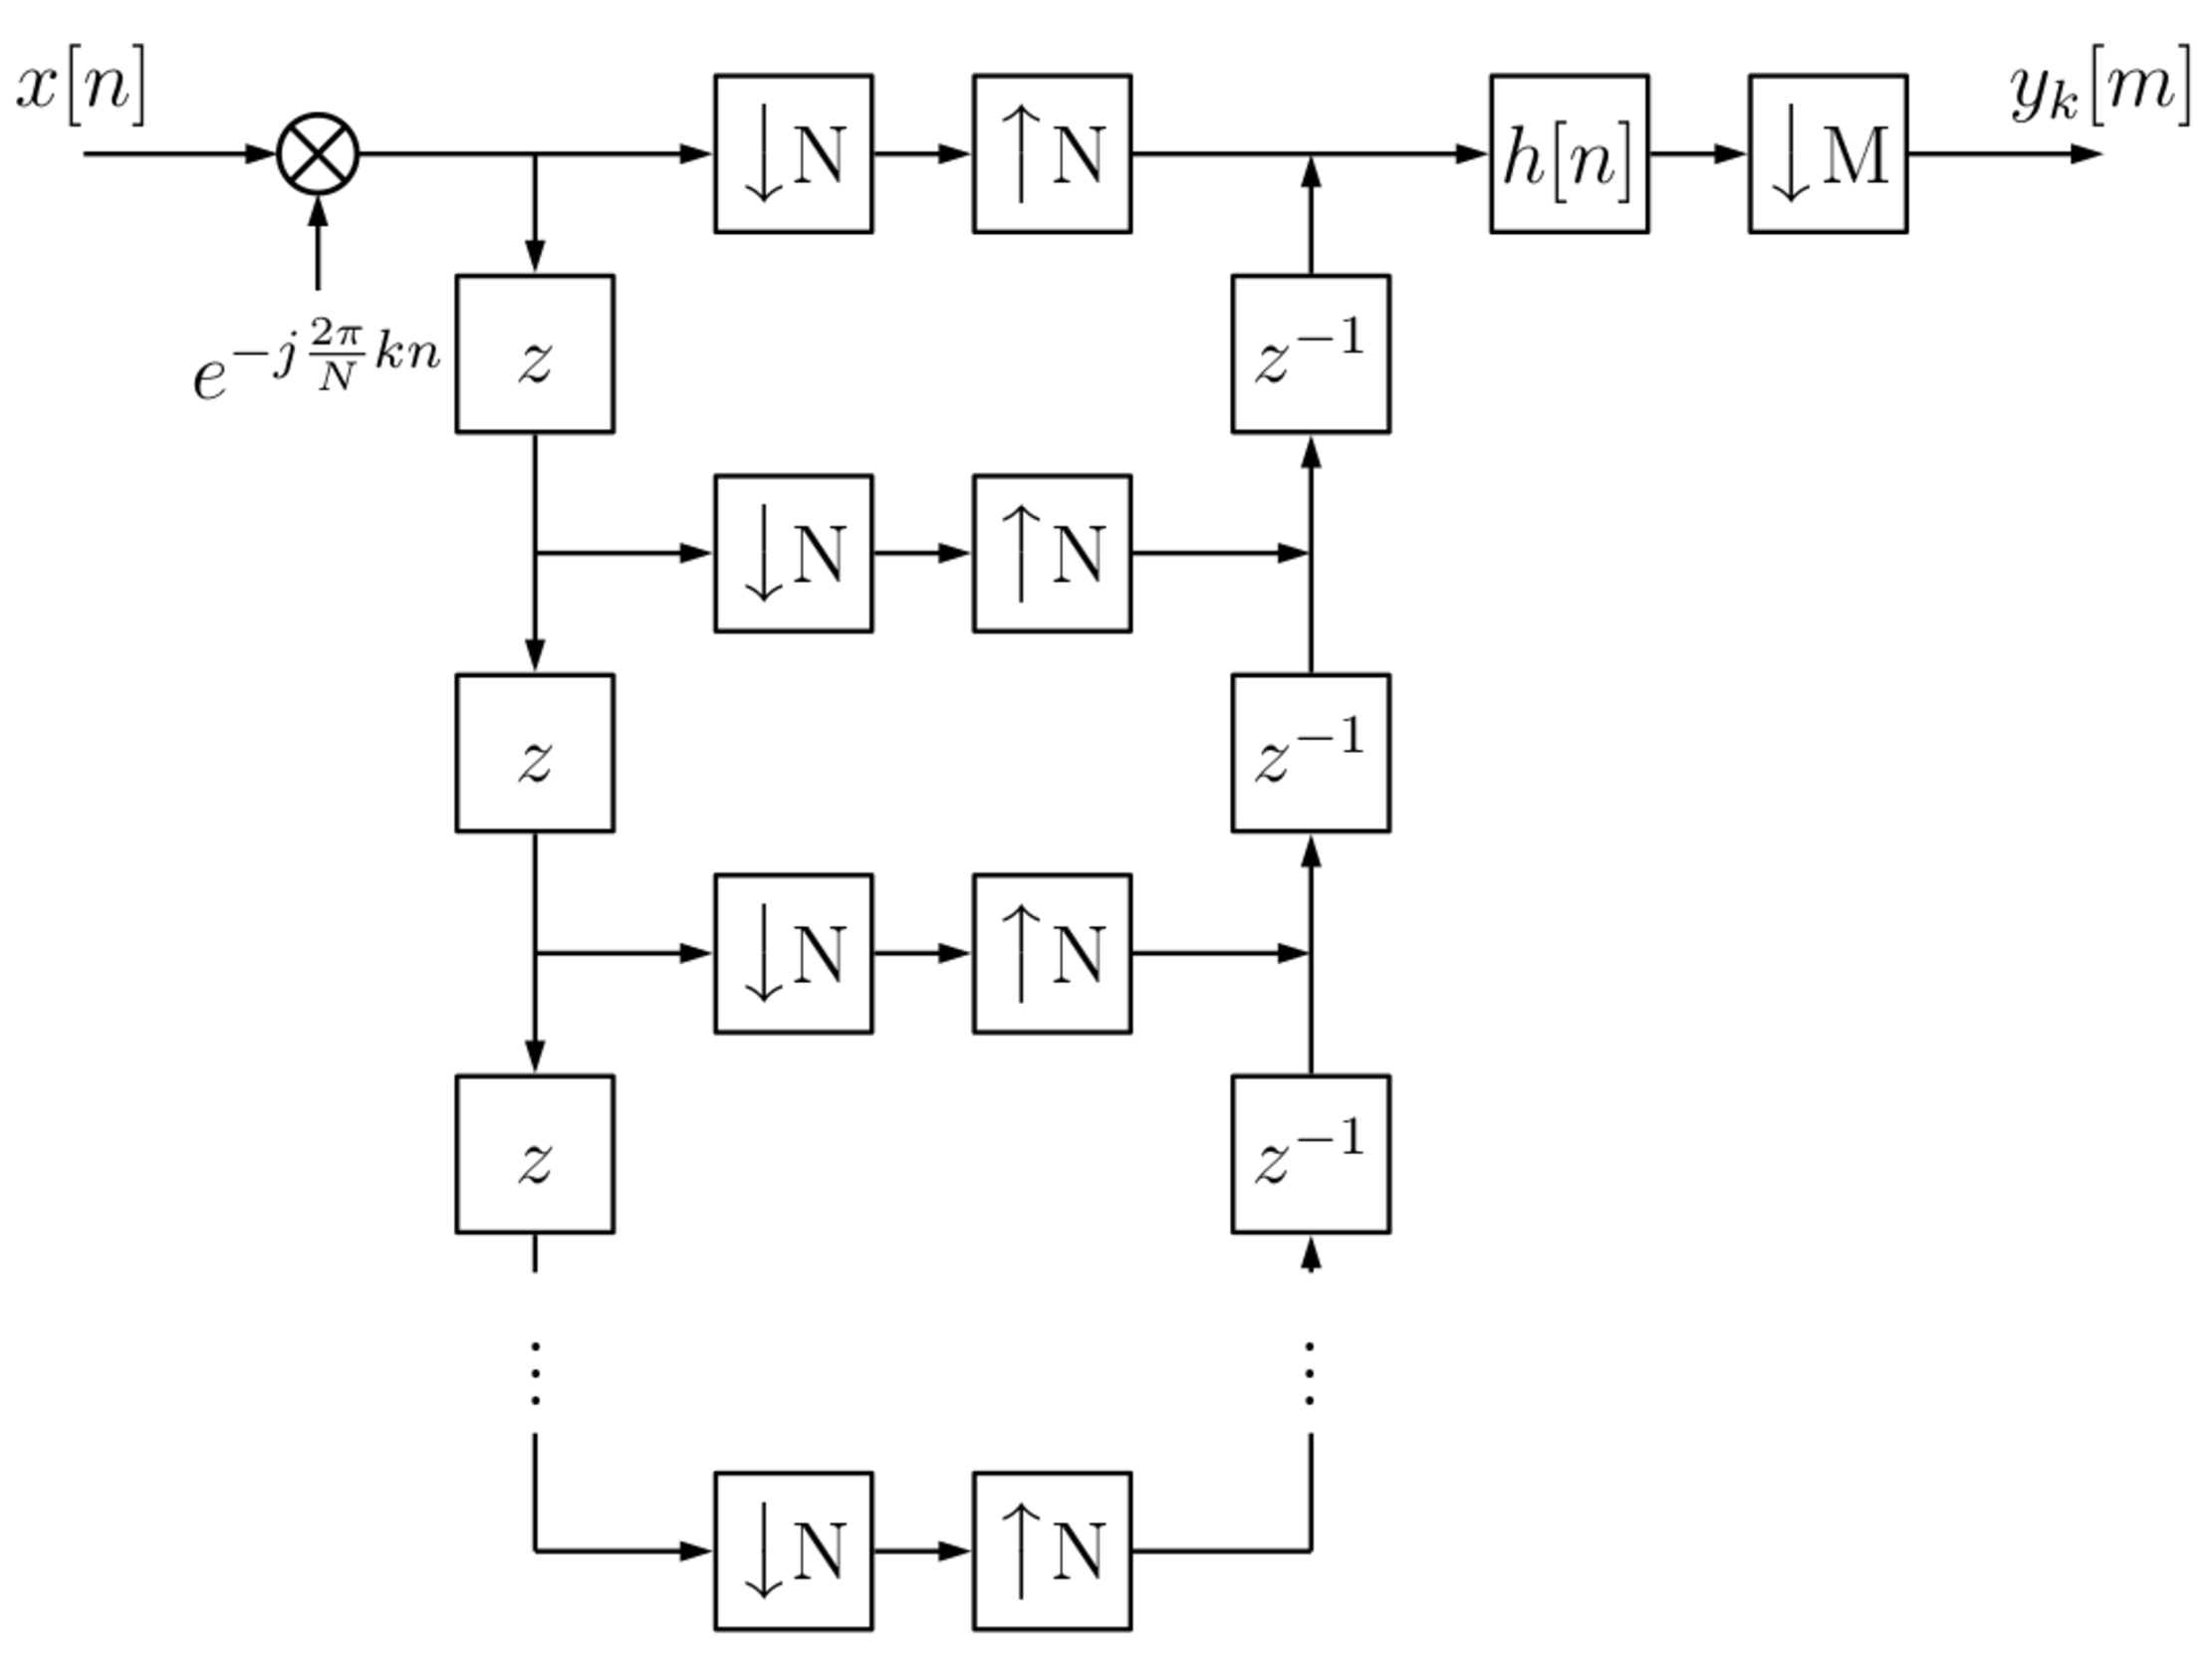
\includegraphics[width=0.8\textwidth]{PFB_opening_after_modulation}}
								\end{center}
\end{frame}

\section{Vivado}
\begin{frame}{Vivado}

				Actualmente trabajando con la versi\'on 2016.4

				Cores propios, ej. RxChannelizer y TxChannelizer, etc.

				Mezcla de scripts TCL y Linux embebido
				\begin{center}
								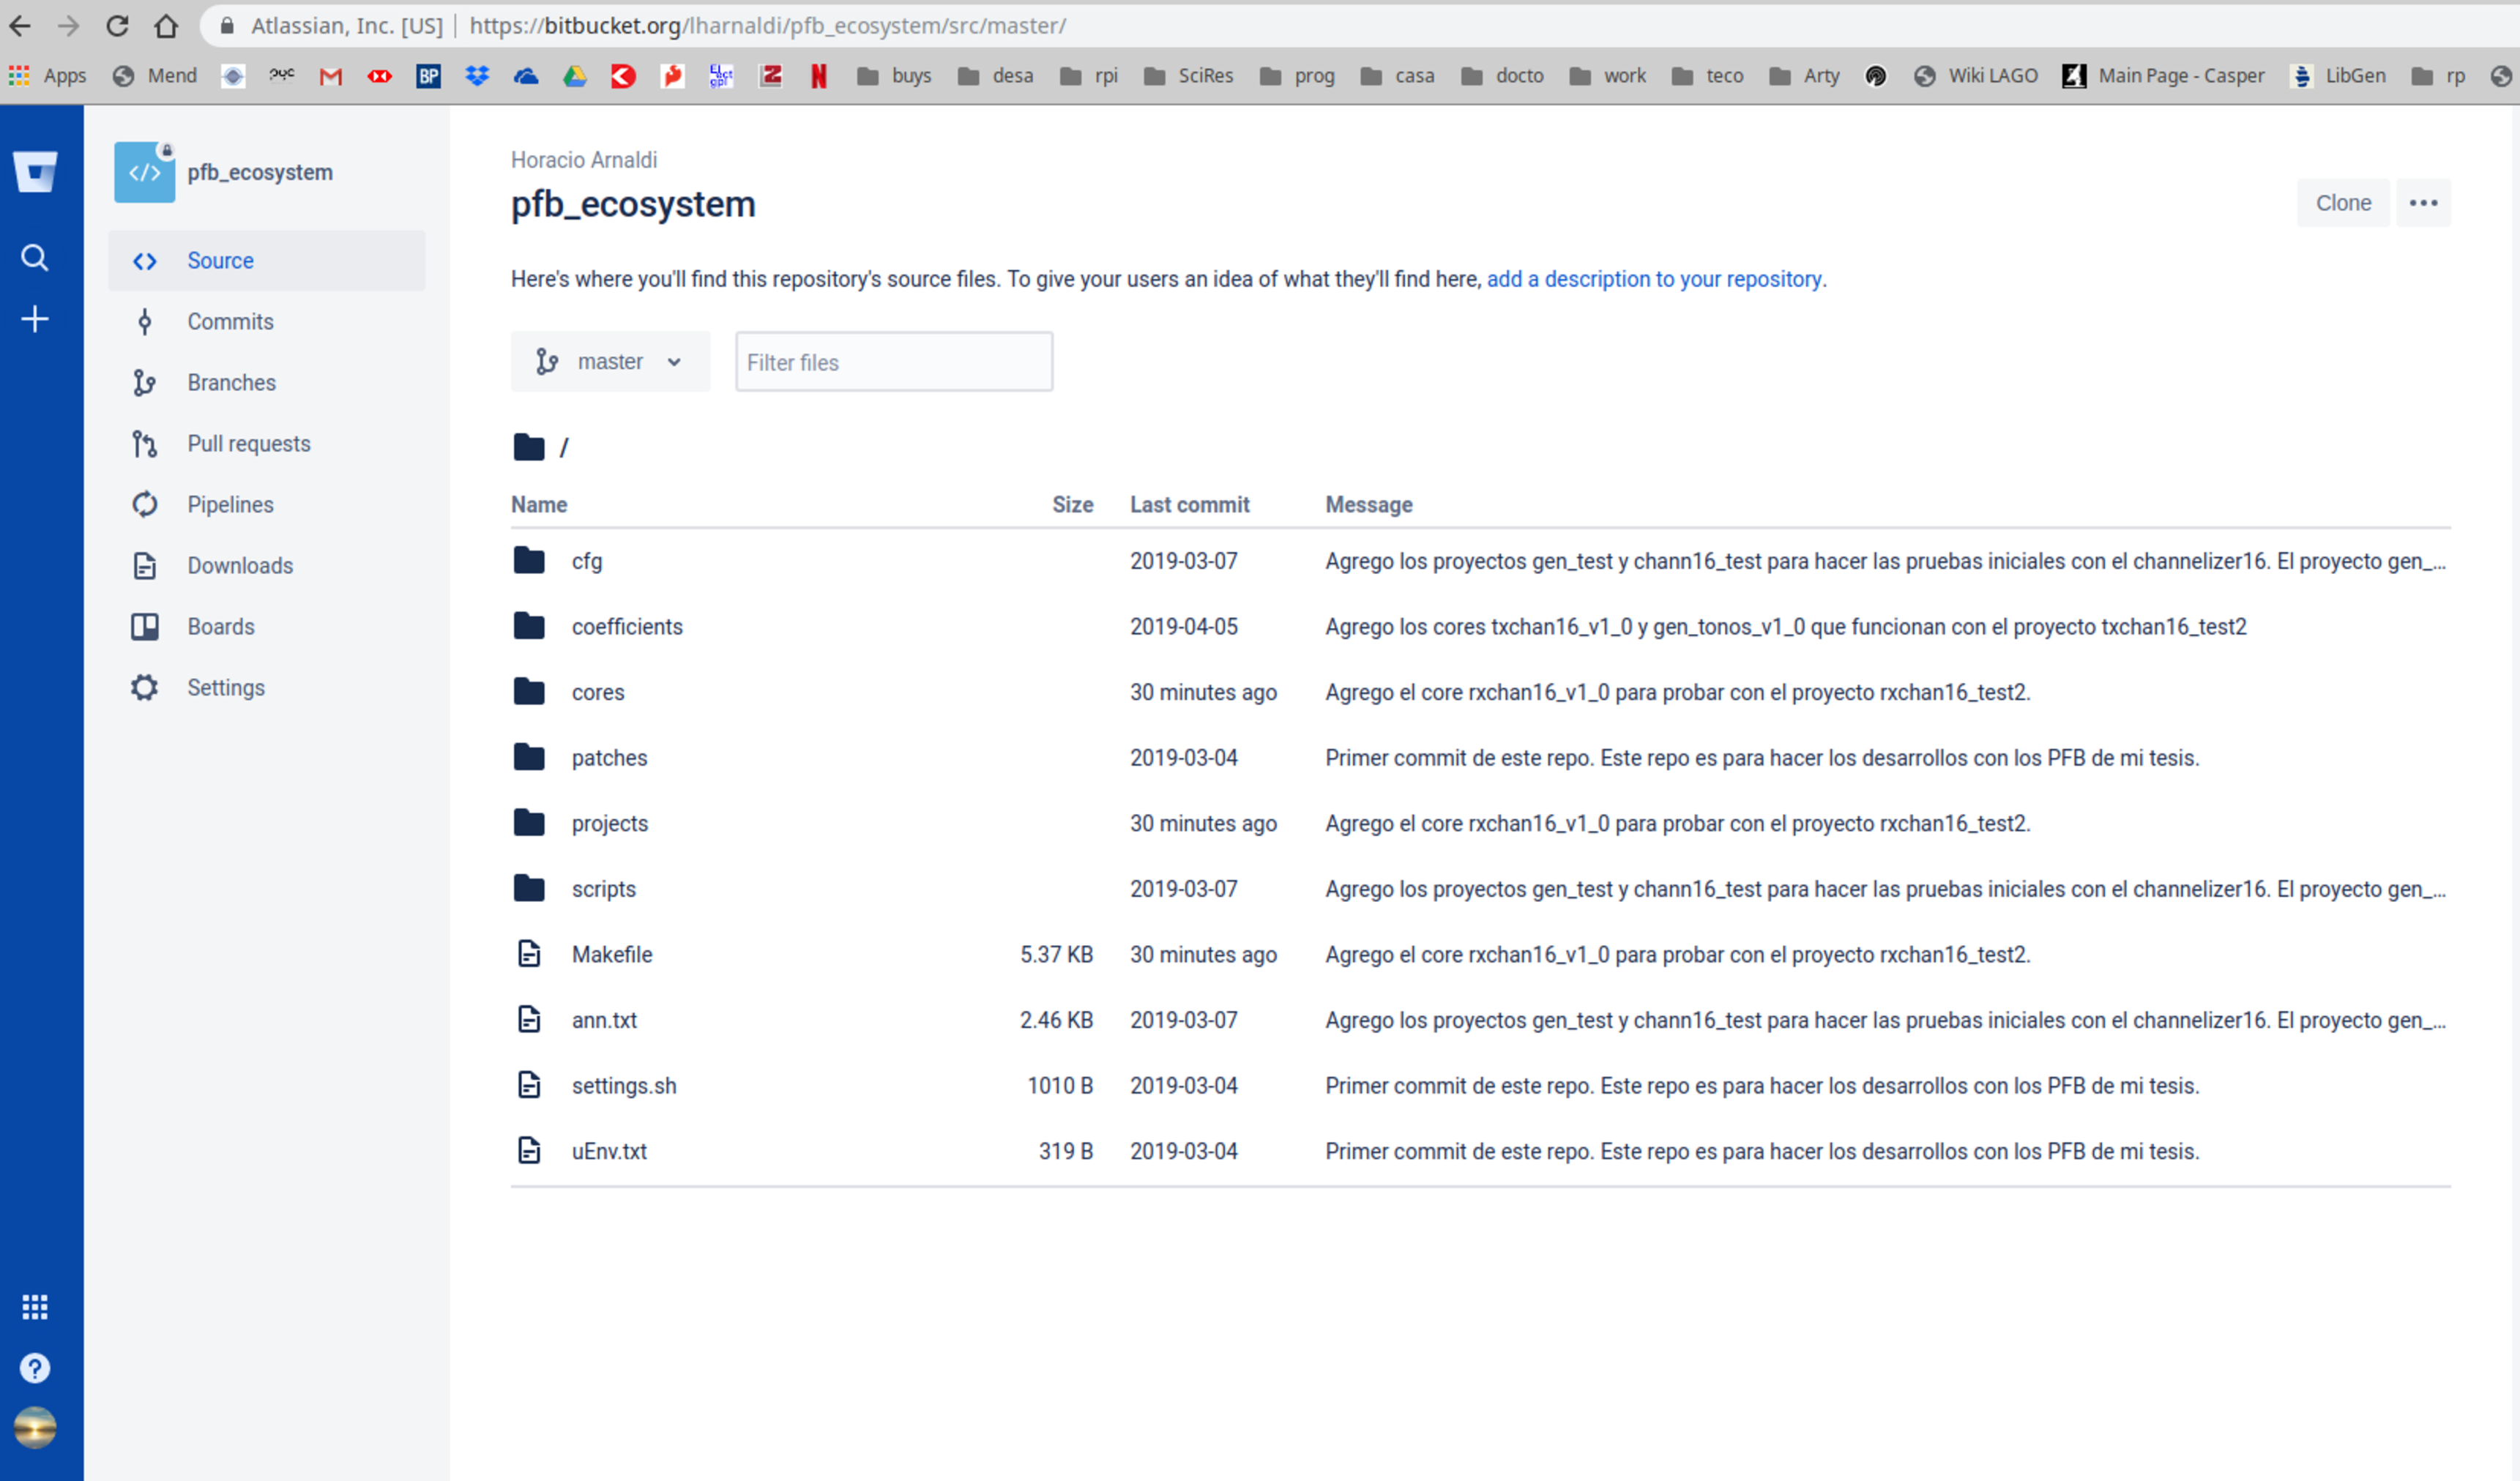
\includegraphics[width=0.8\textwidth]{pfb_repo}
				\end{center}
\end{frame}

\begin{frame}{Proyectos Vivado}

				%\begin{columns}
				%\begin{column}{0.45\textwidth}
				\begin{center}
								\only<1>{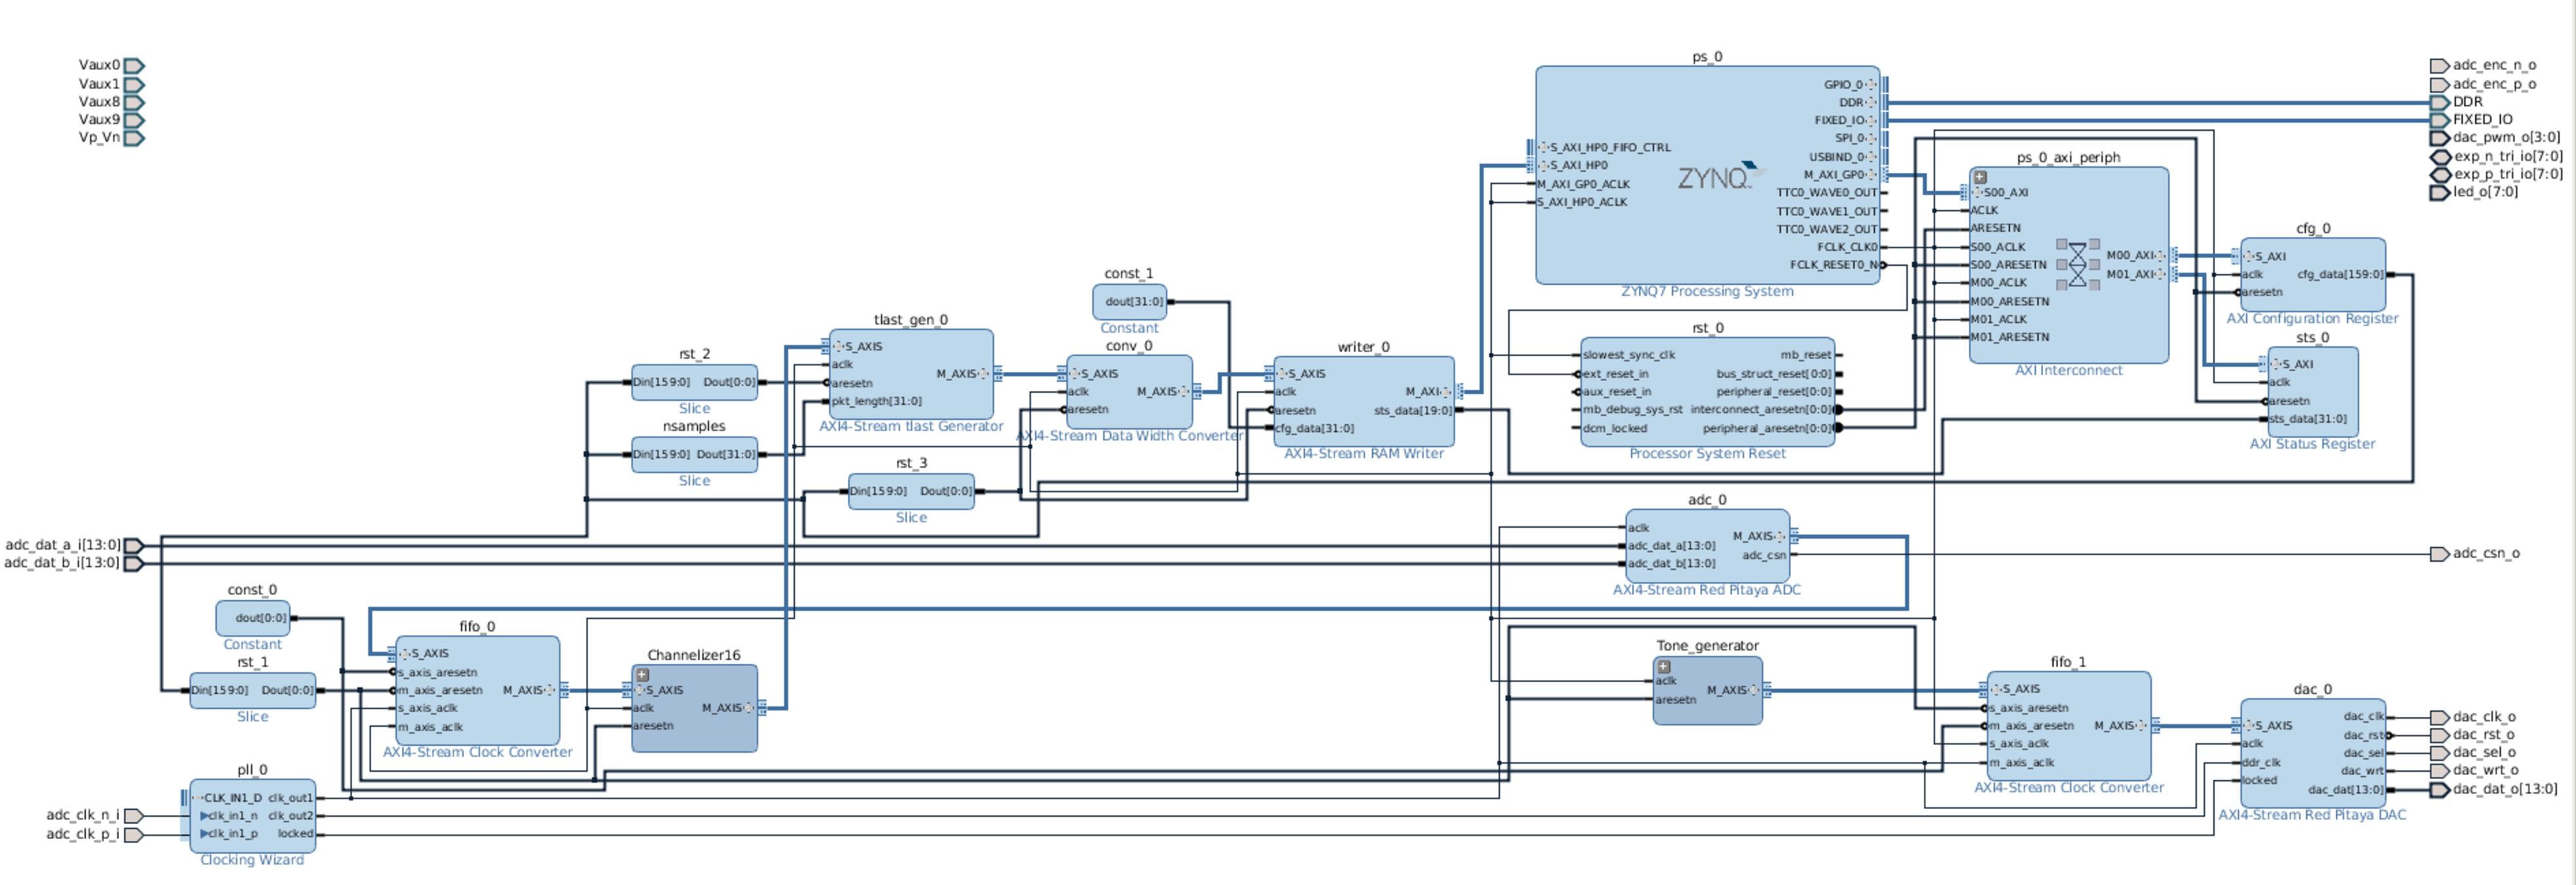
\includegraphics[width=0.95\textwidth]{rxchan16_test2_vivado_project}}
				\end{center}
				%\end{column}
				%\begin{column}{0.45\textwidth}
								\begin{center}
												\only<2>{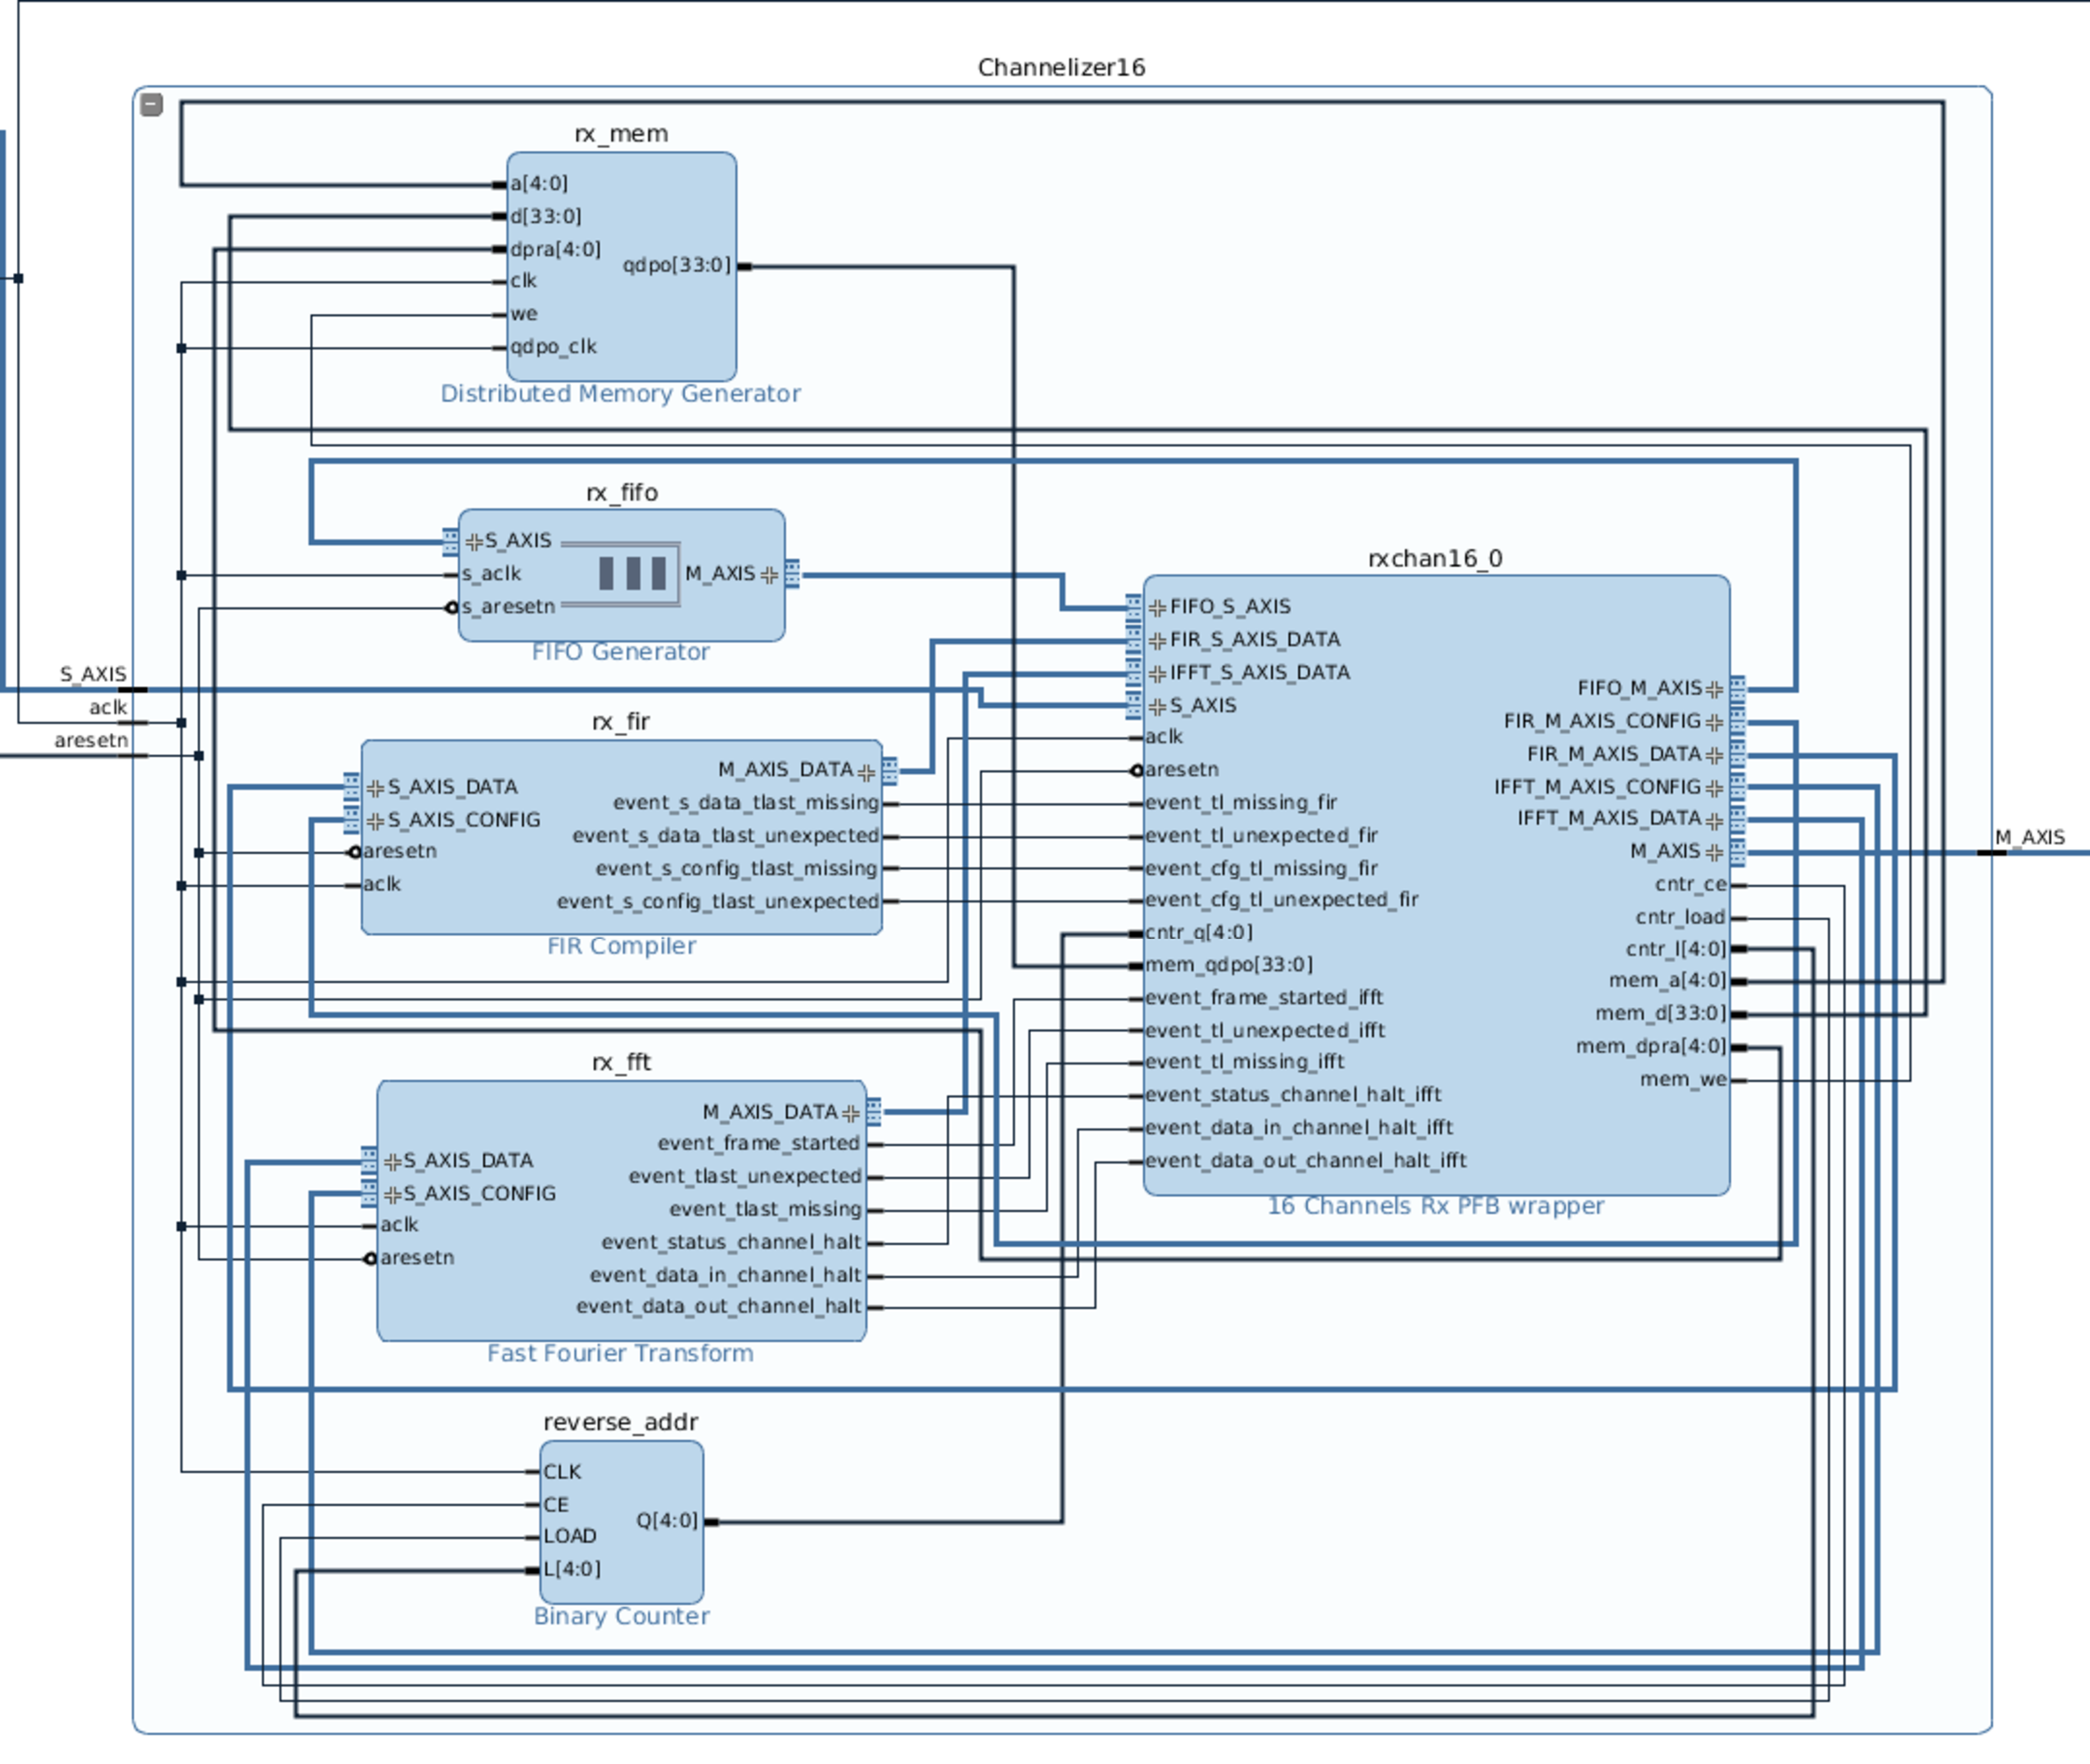
\includegraphics[width=0.8\textwidth]{channelizer16_core}}
								\end{center}
								%\end{column}
								%\end{columns}
\end{frame}

\section{Amplificador de bajo ruido}
\begin{frame}{Amplificador}
				\begin{columns}
								\begin{column}{0.45\textwidth}
												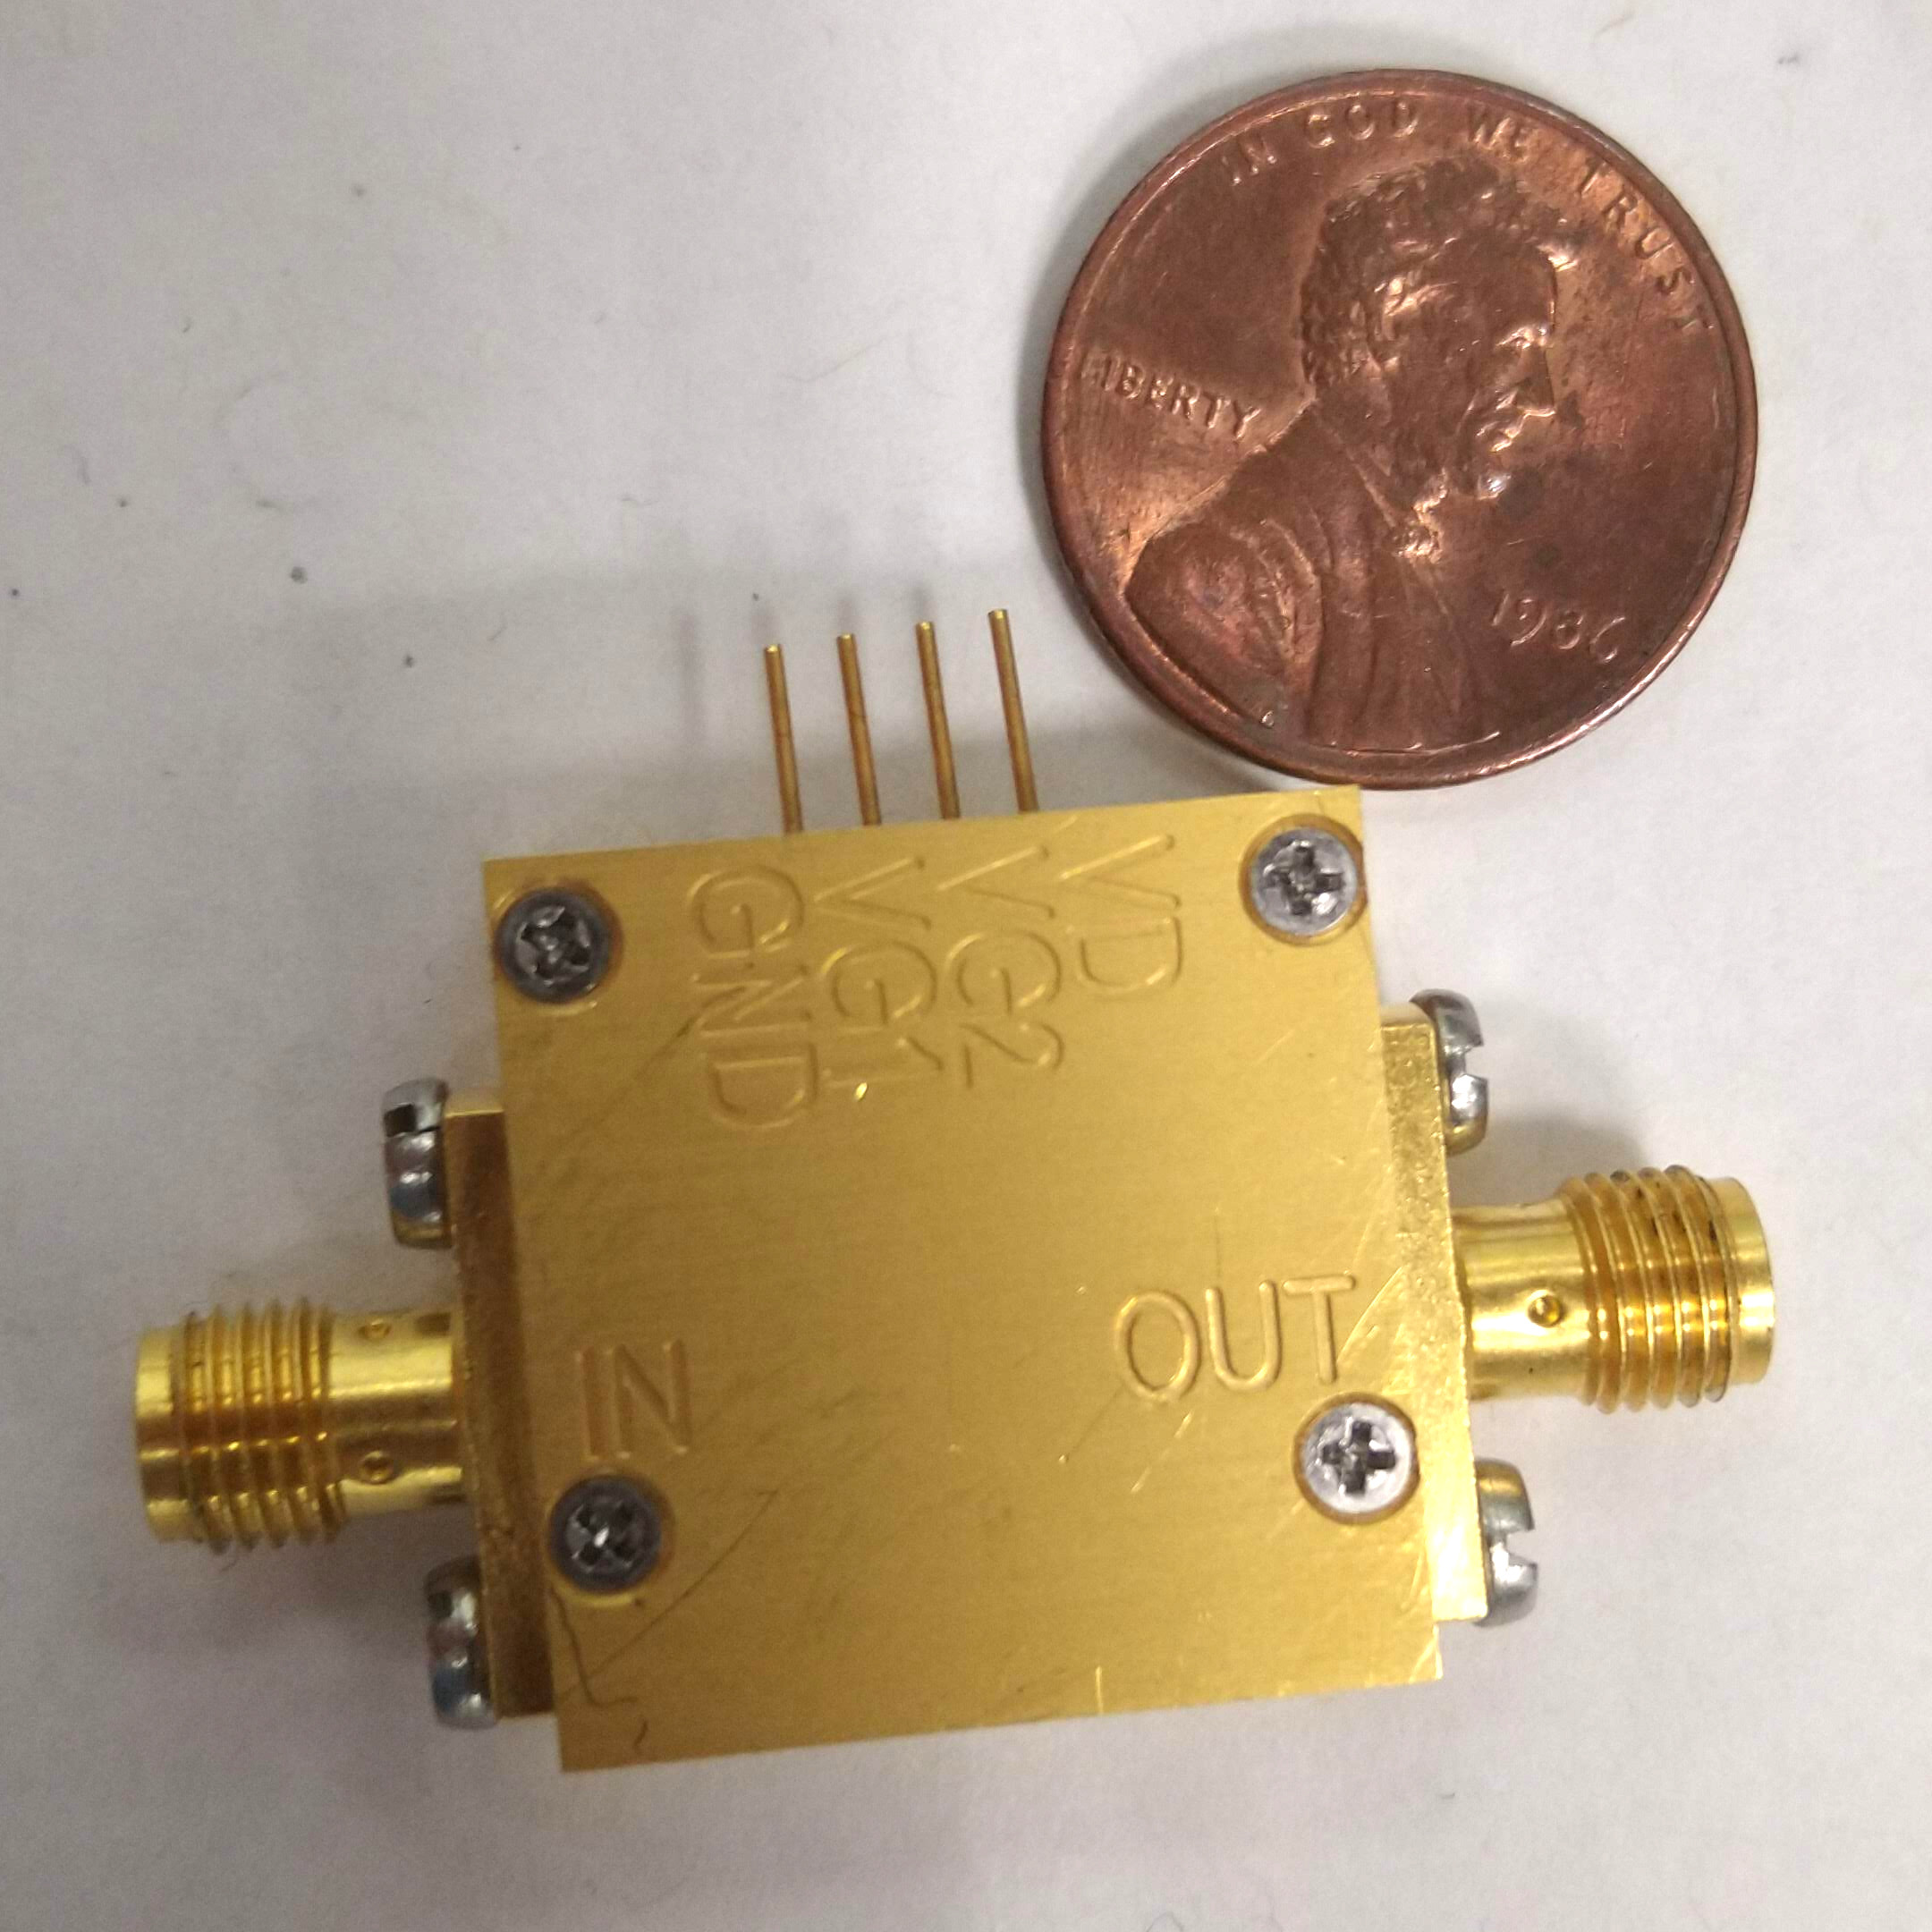
\includegraphics[angle=-90,width=0.62\textwidth]{amp_low_temp1} \\ 
												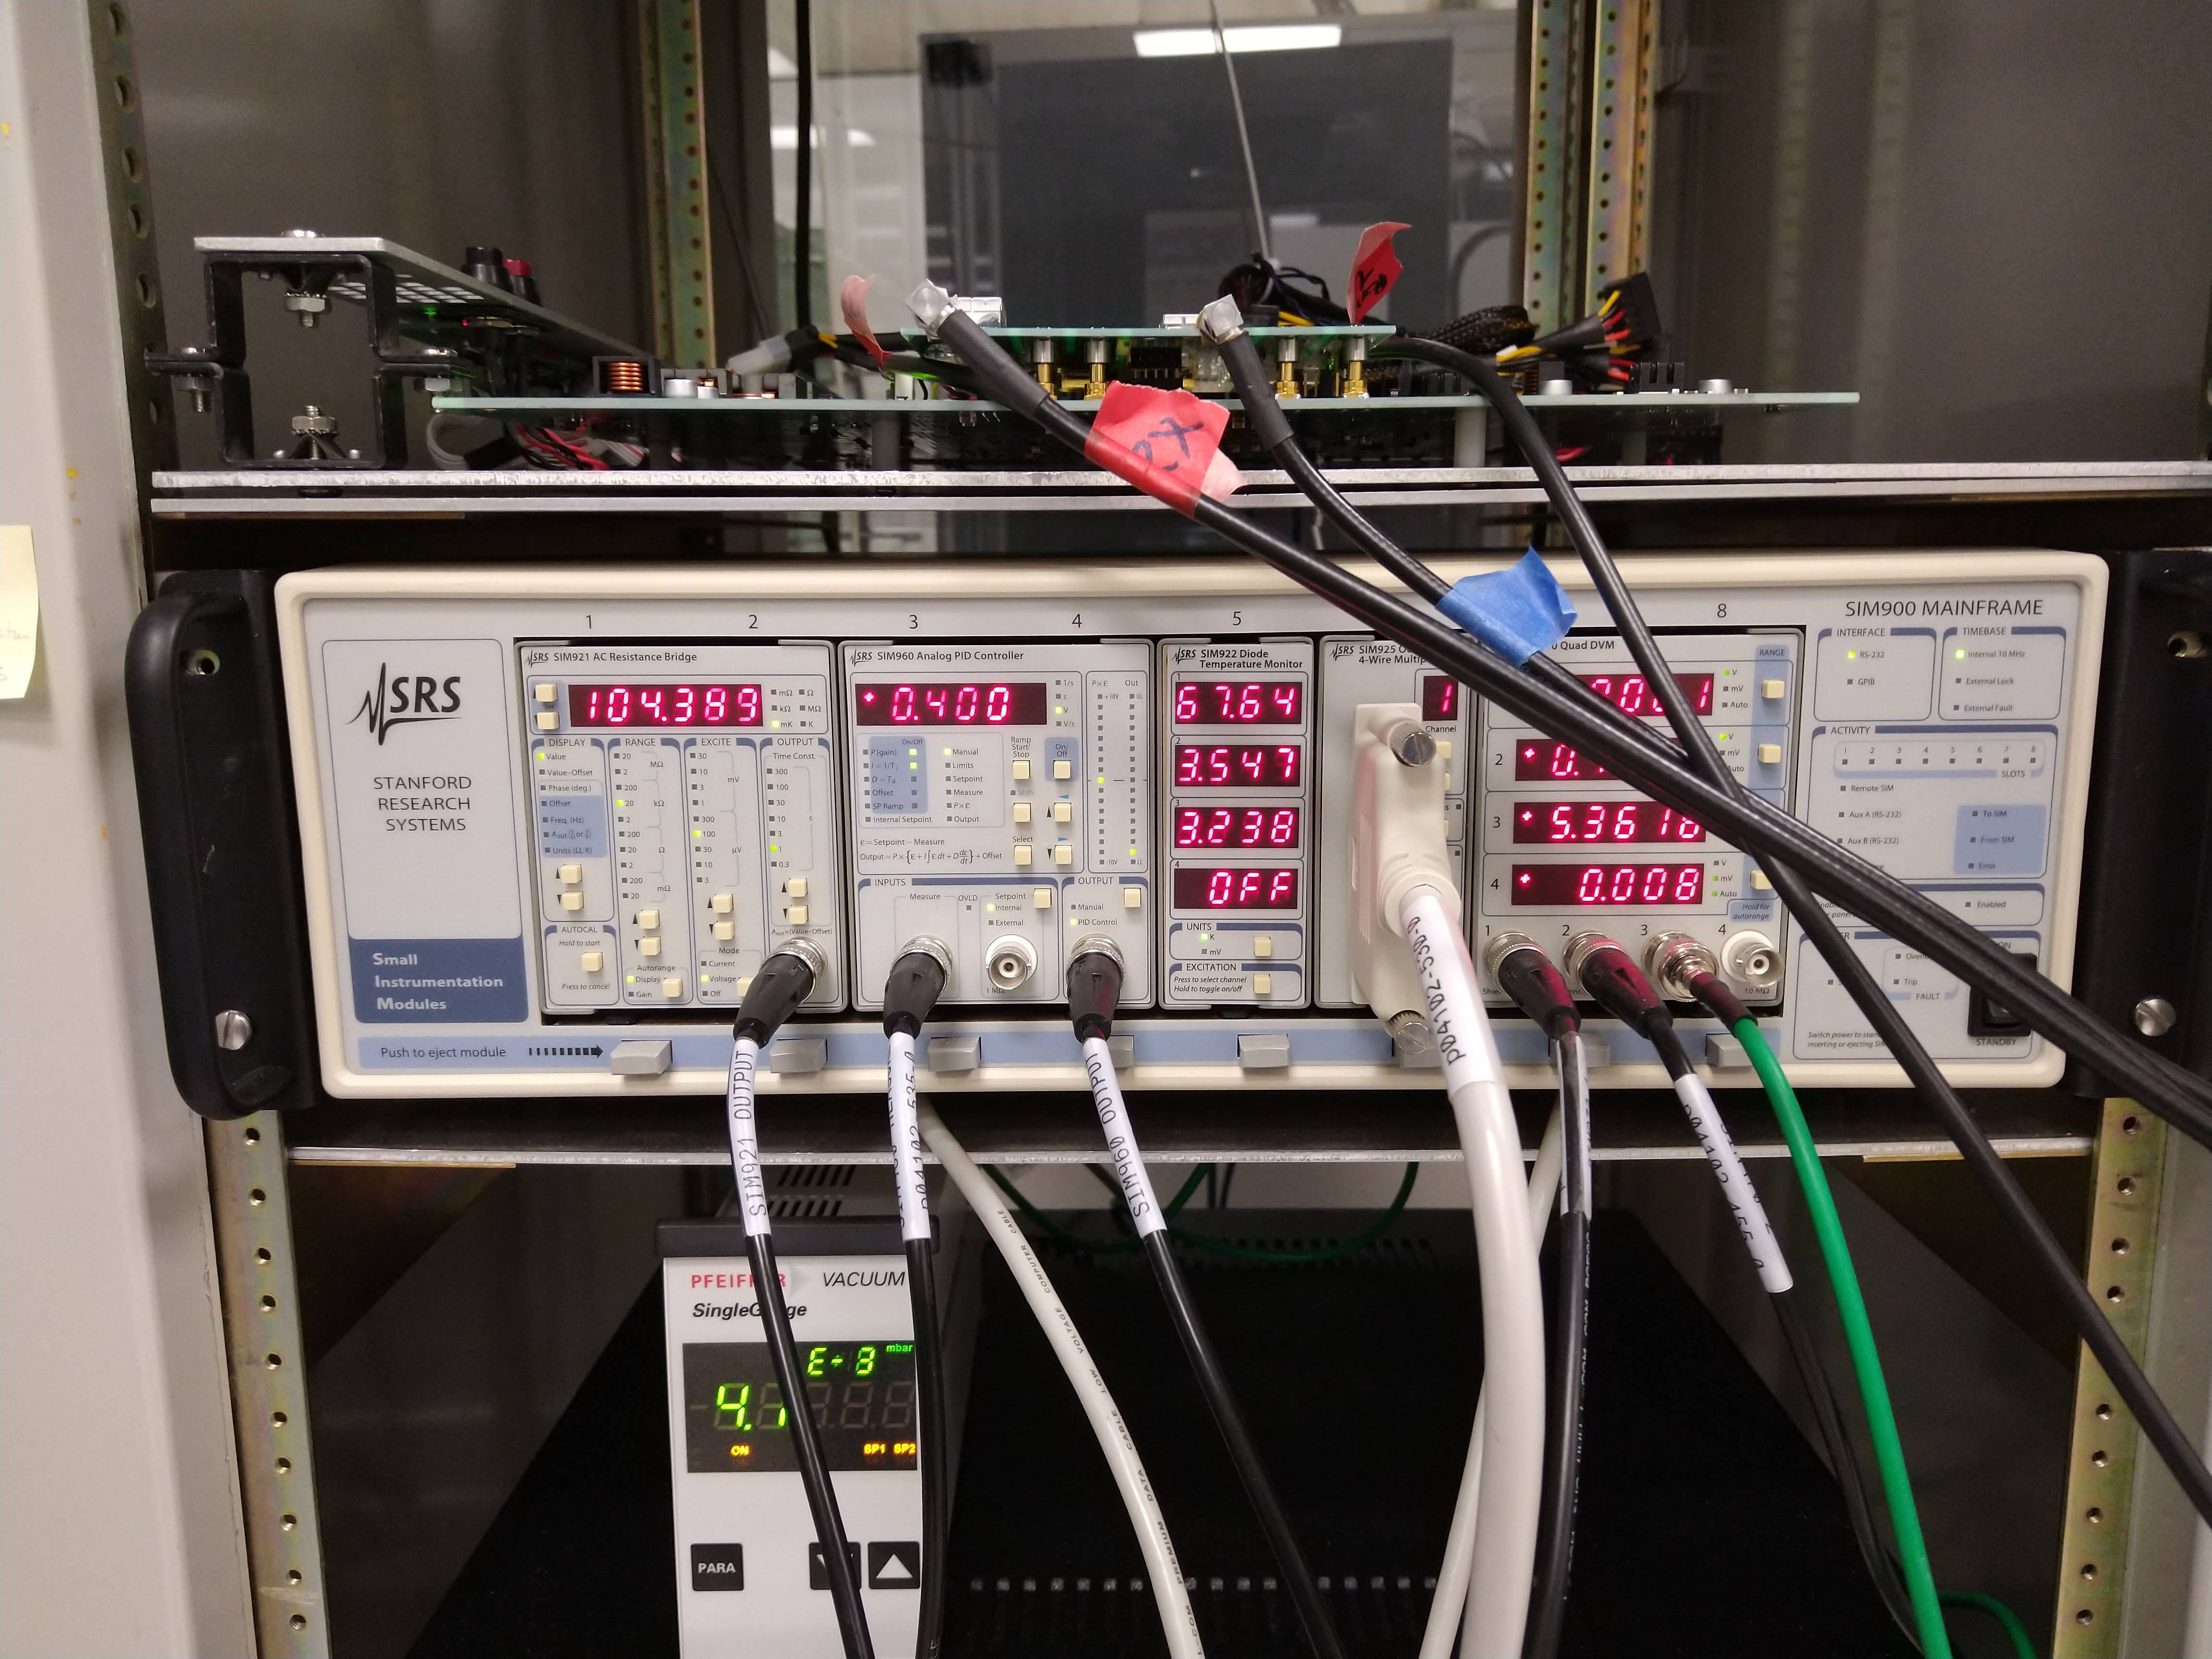
\includegraphics[angle=-90,width=0.6\textwidth]{sim900_mainframe_med_temp}
								\end{column}
								\begin{column}{0.45\textwidth}
												\includegraphics[angle=-90,width=0.62\textwidth]{acople_linea_mkid} \\ 
												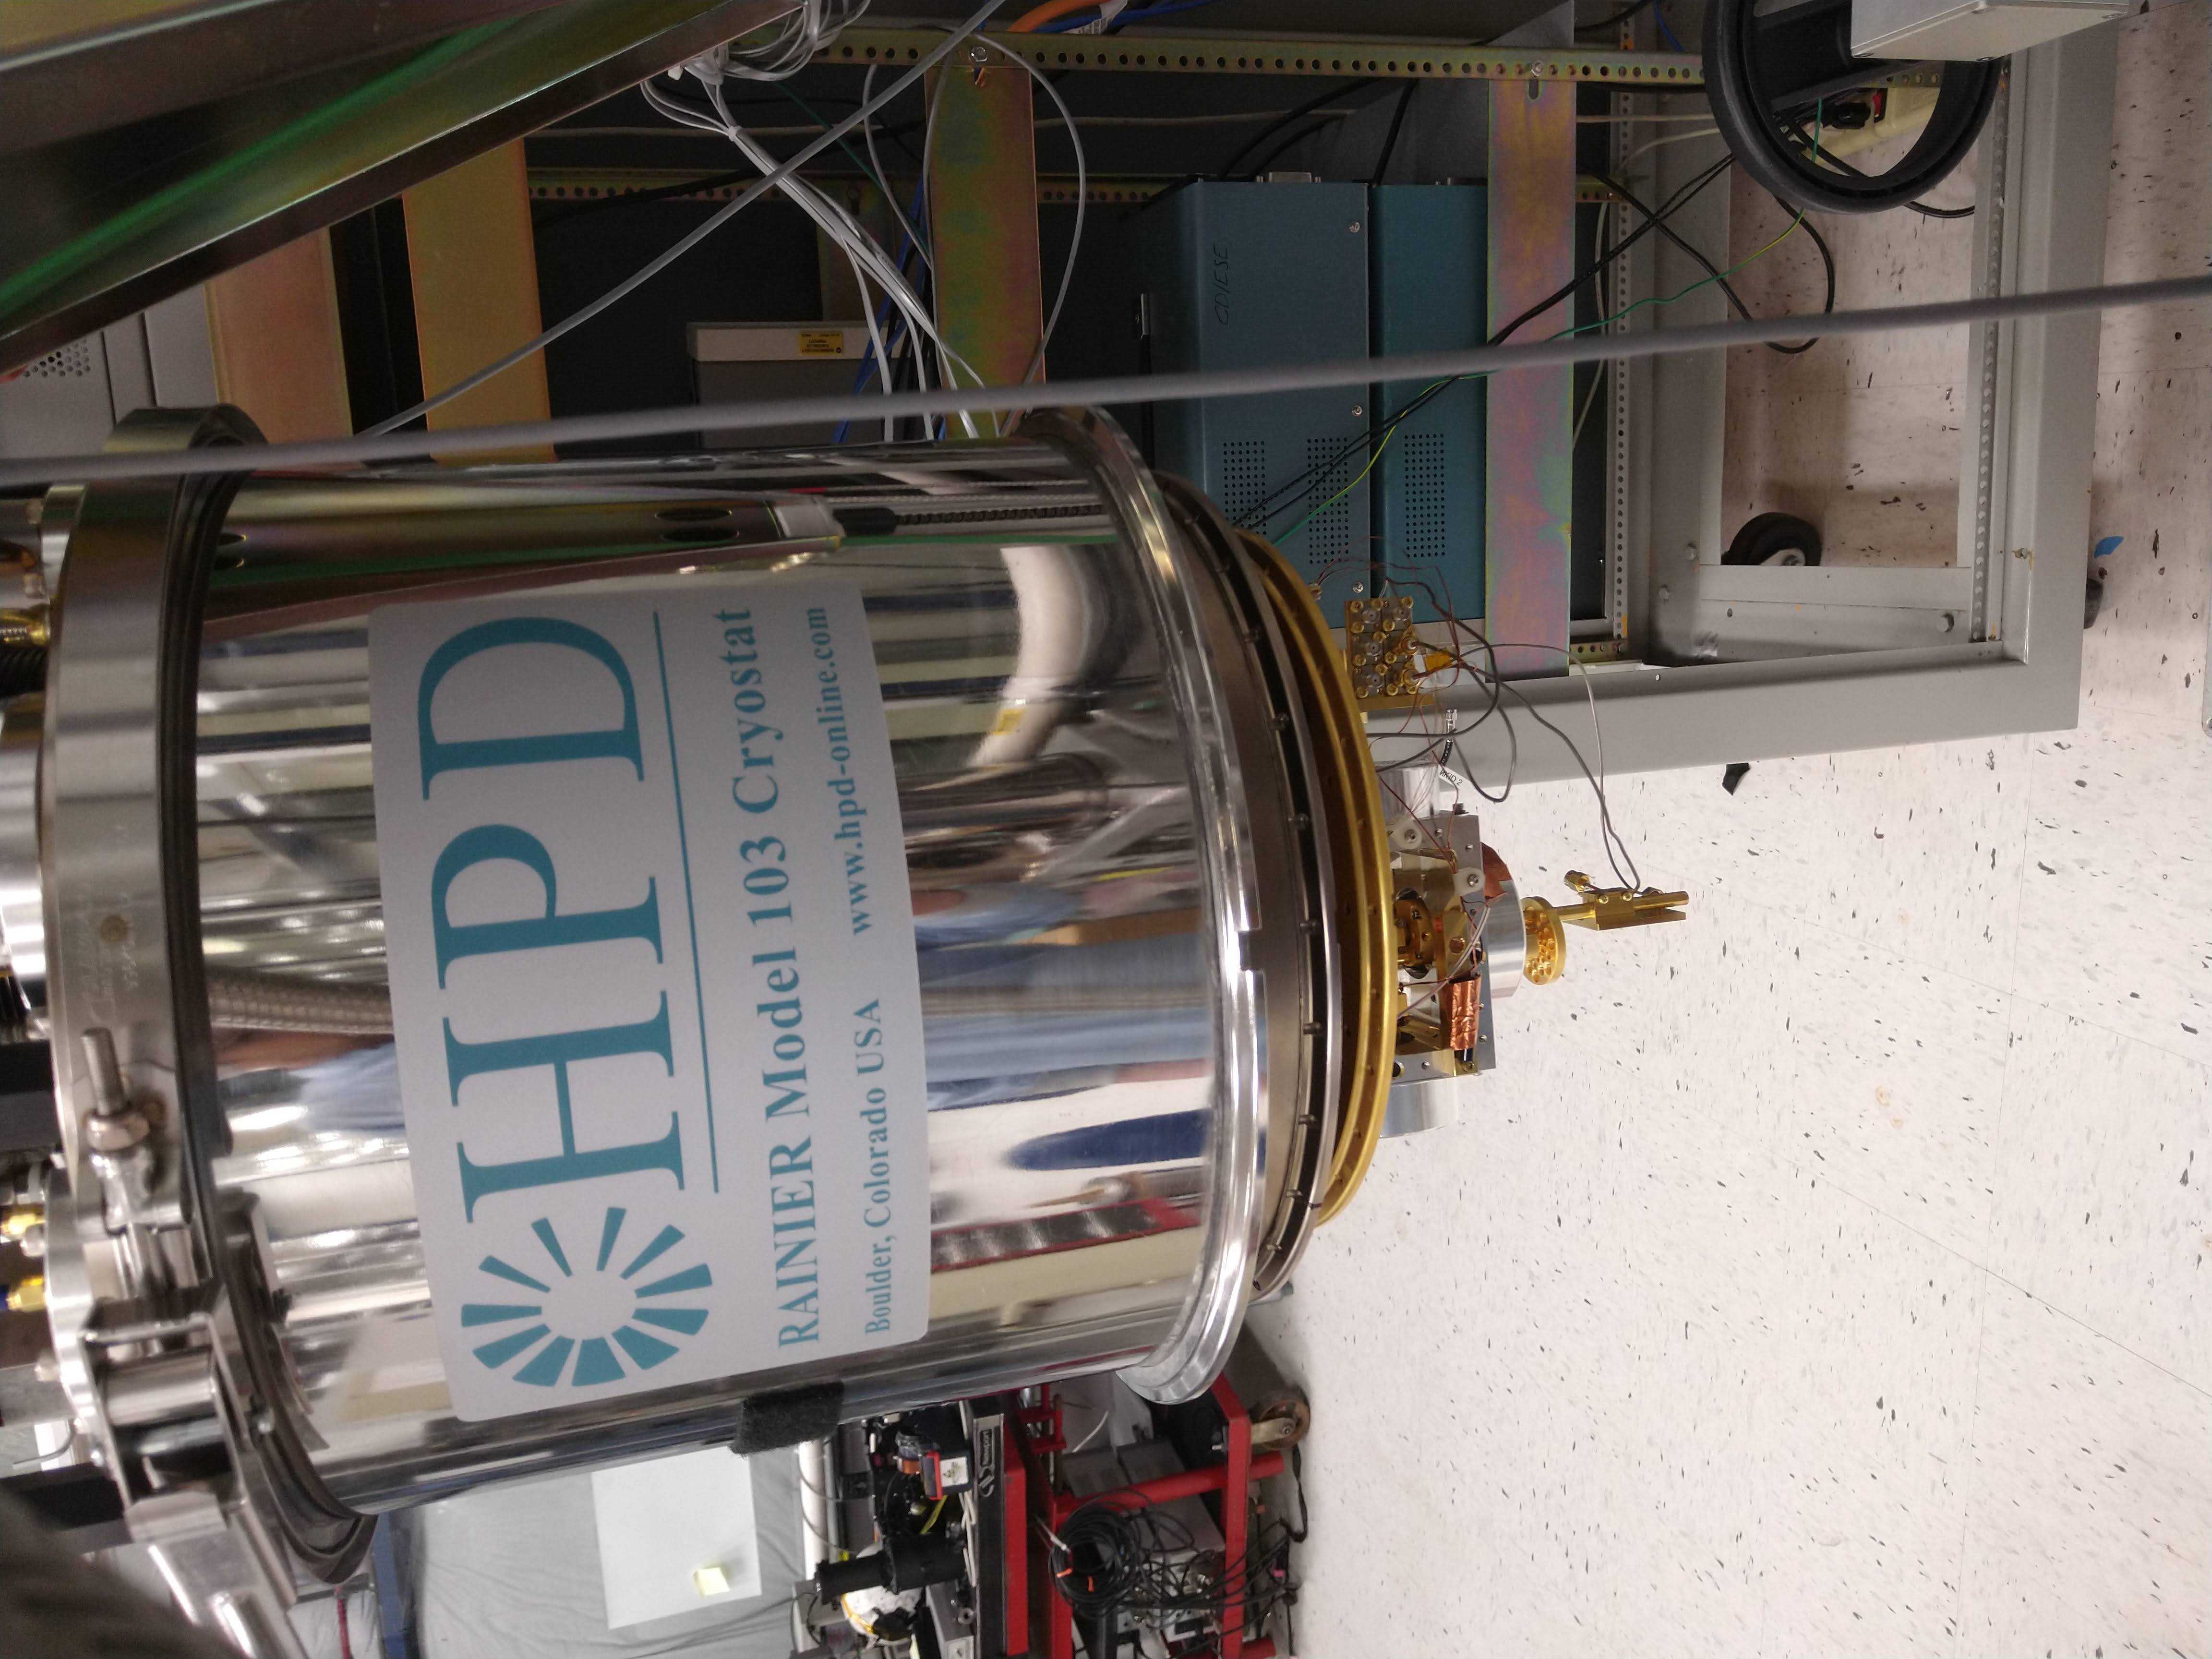
\includegraphics[angle=-90,width=0.6\textwidth]{criostato_modelo}
								\end{column}
				\end{columns}
\end{frame}
\begin{frame}{Amplificador}
				\begin{columns}
								\begin{column}{0.45\textwidth}
												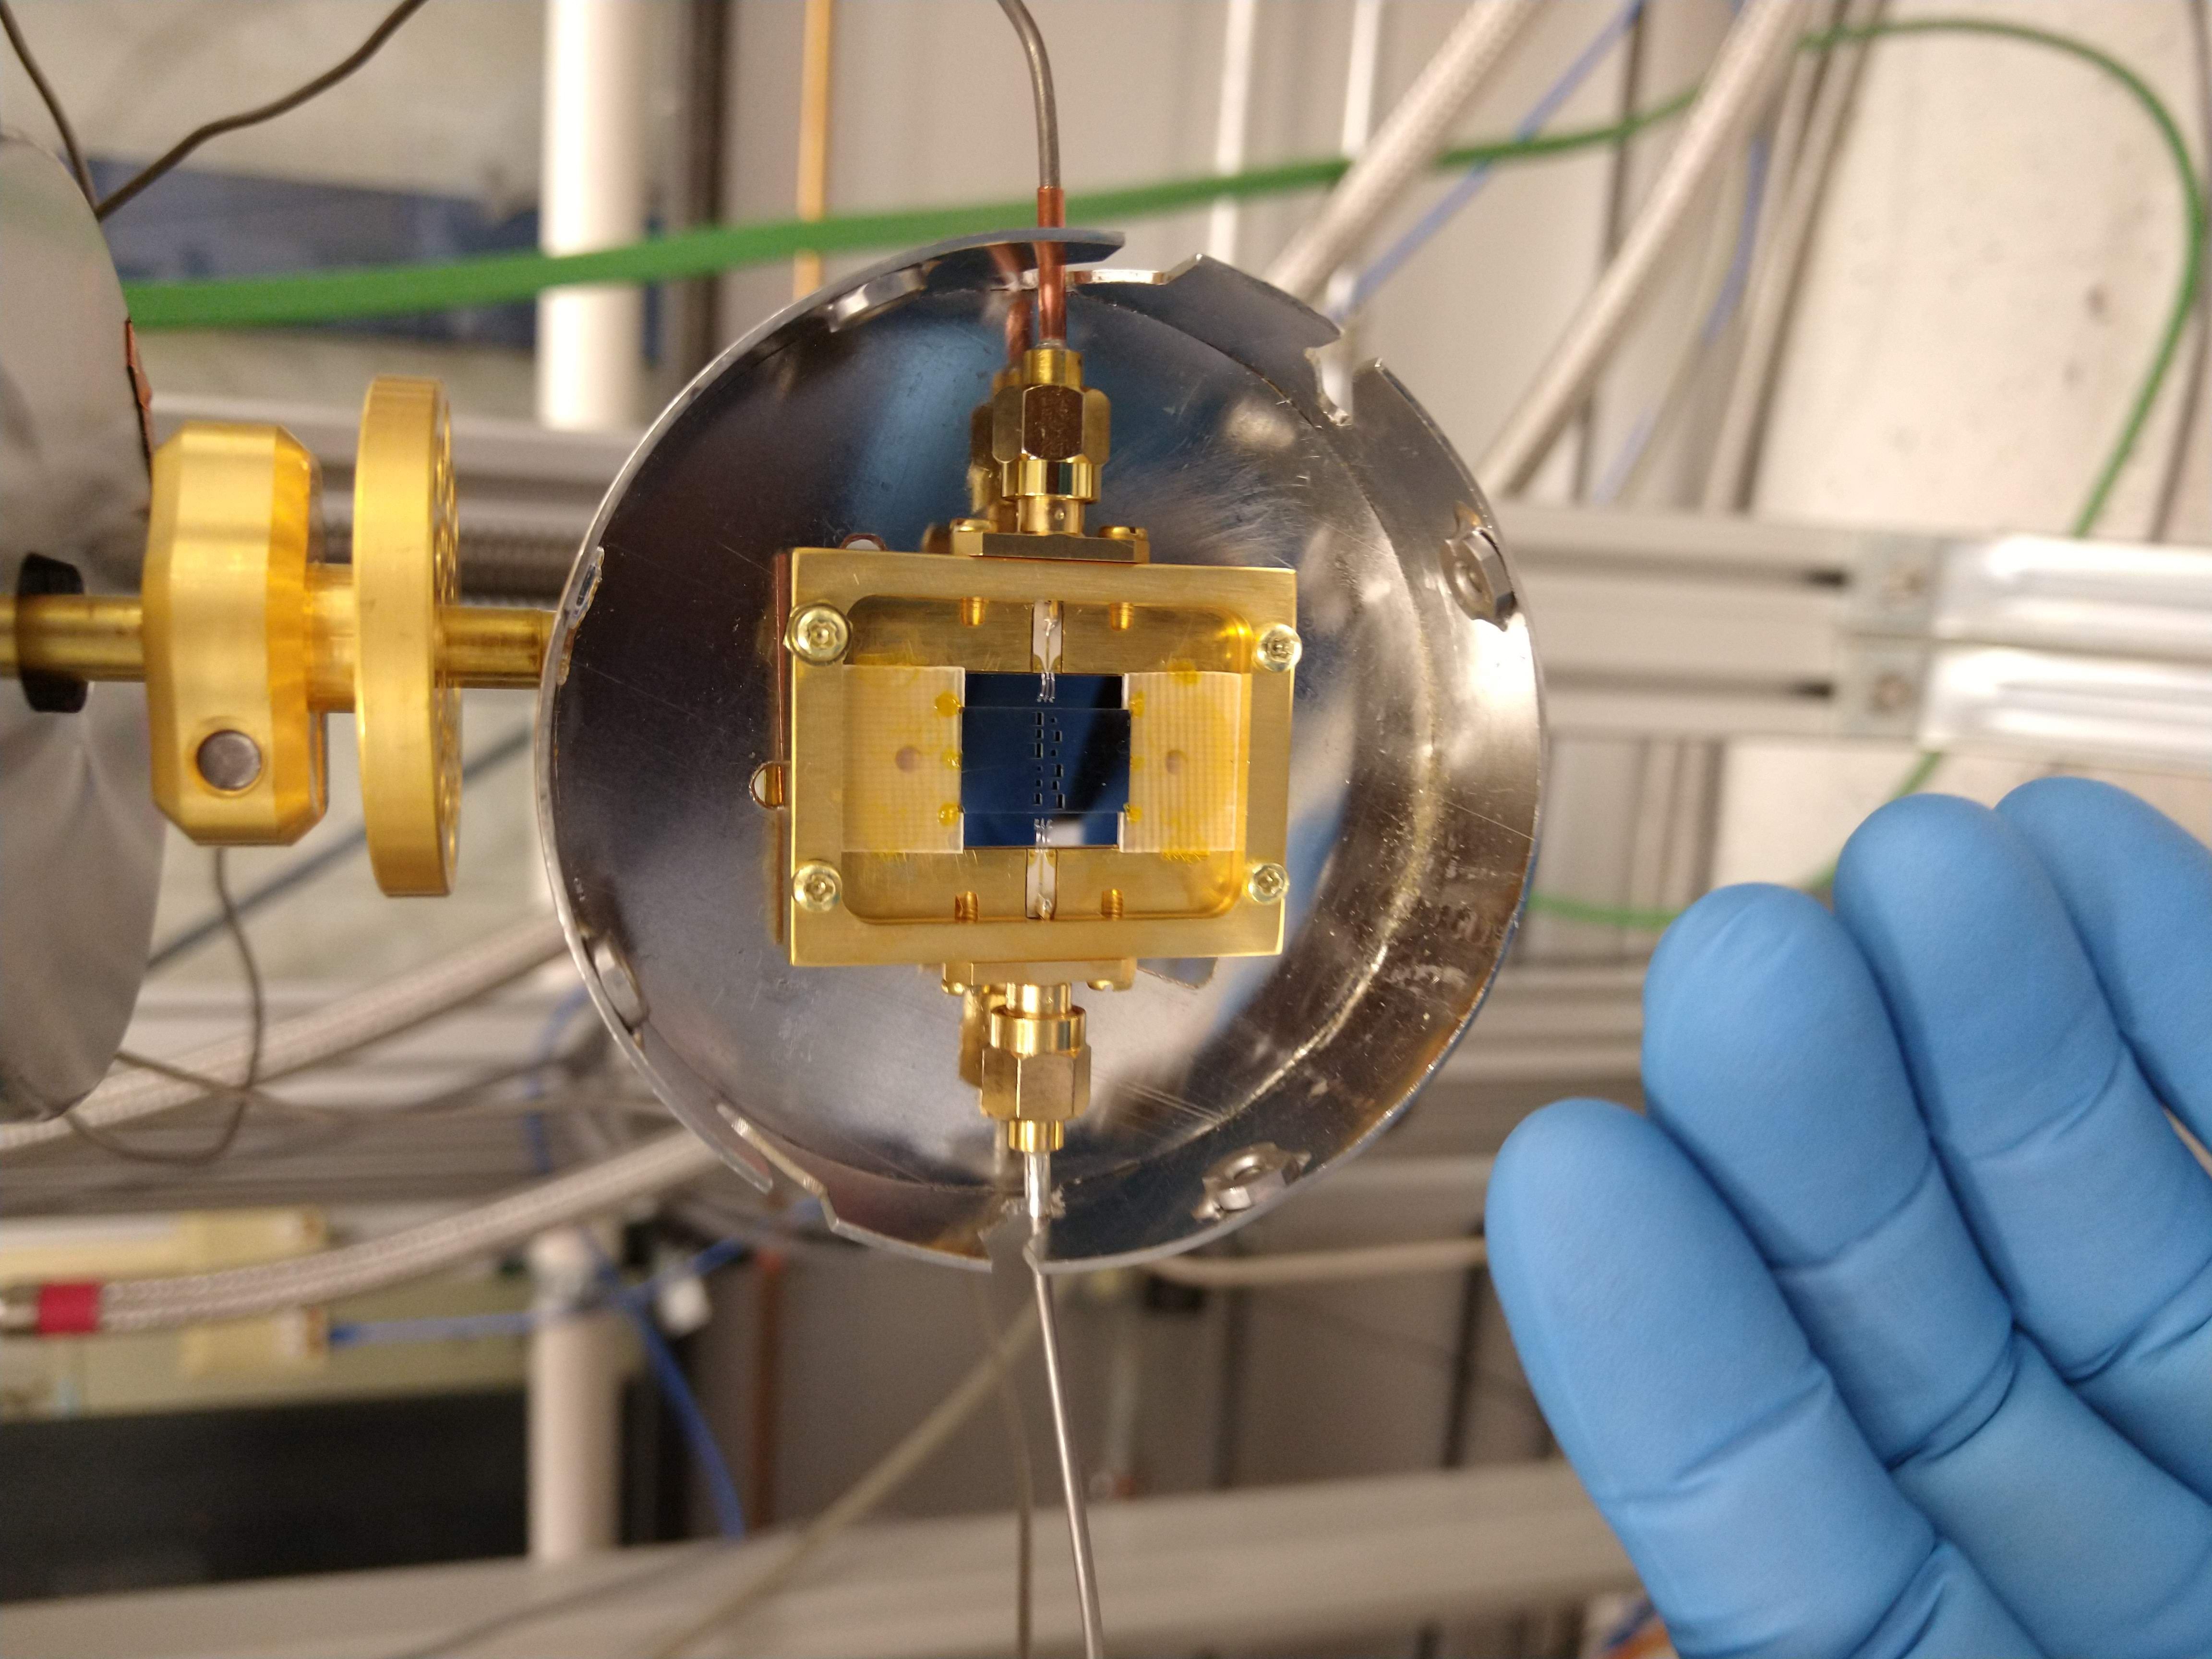
\includegraphics[angle=-90,width=0.62\textwidth]{mkid1} \\ 
												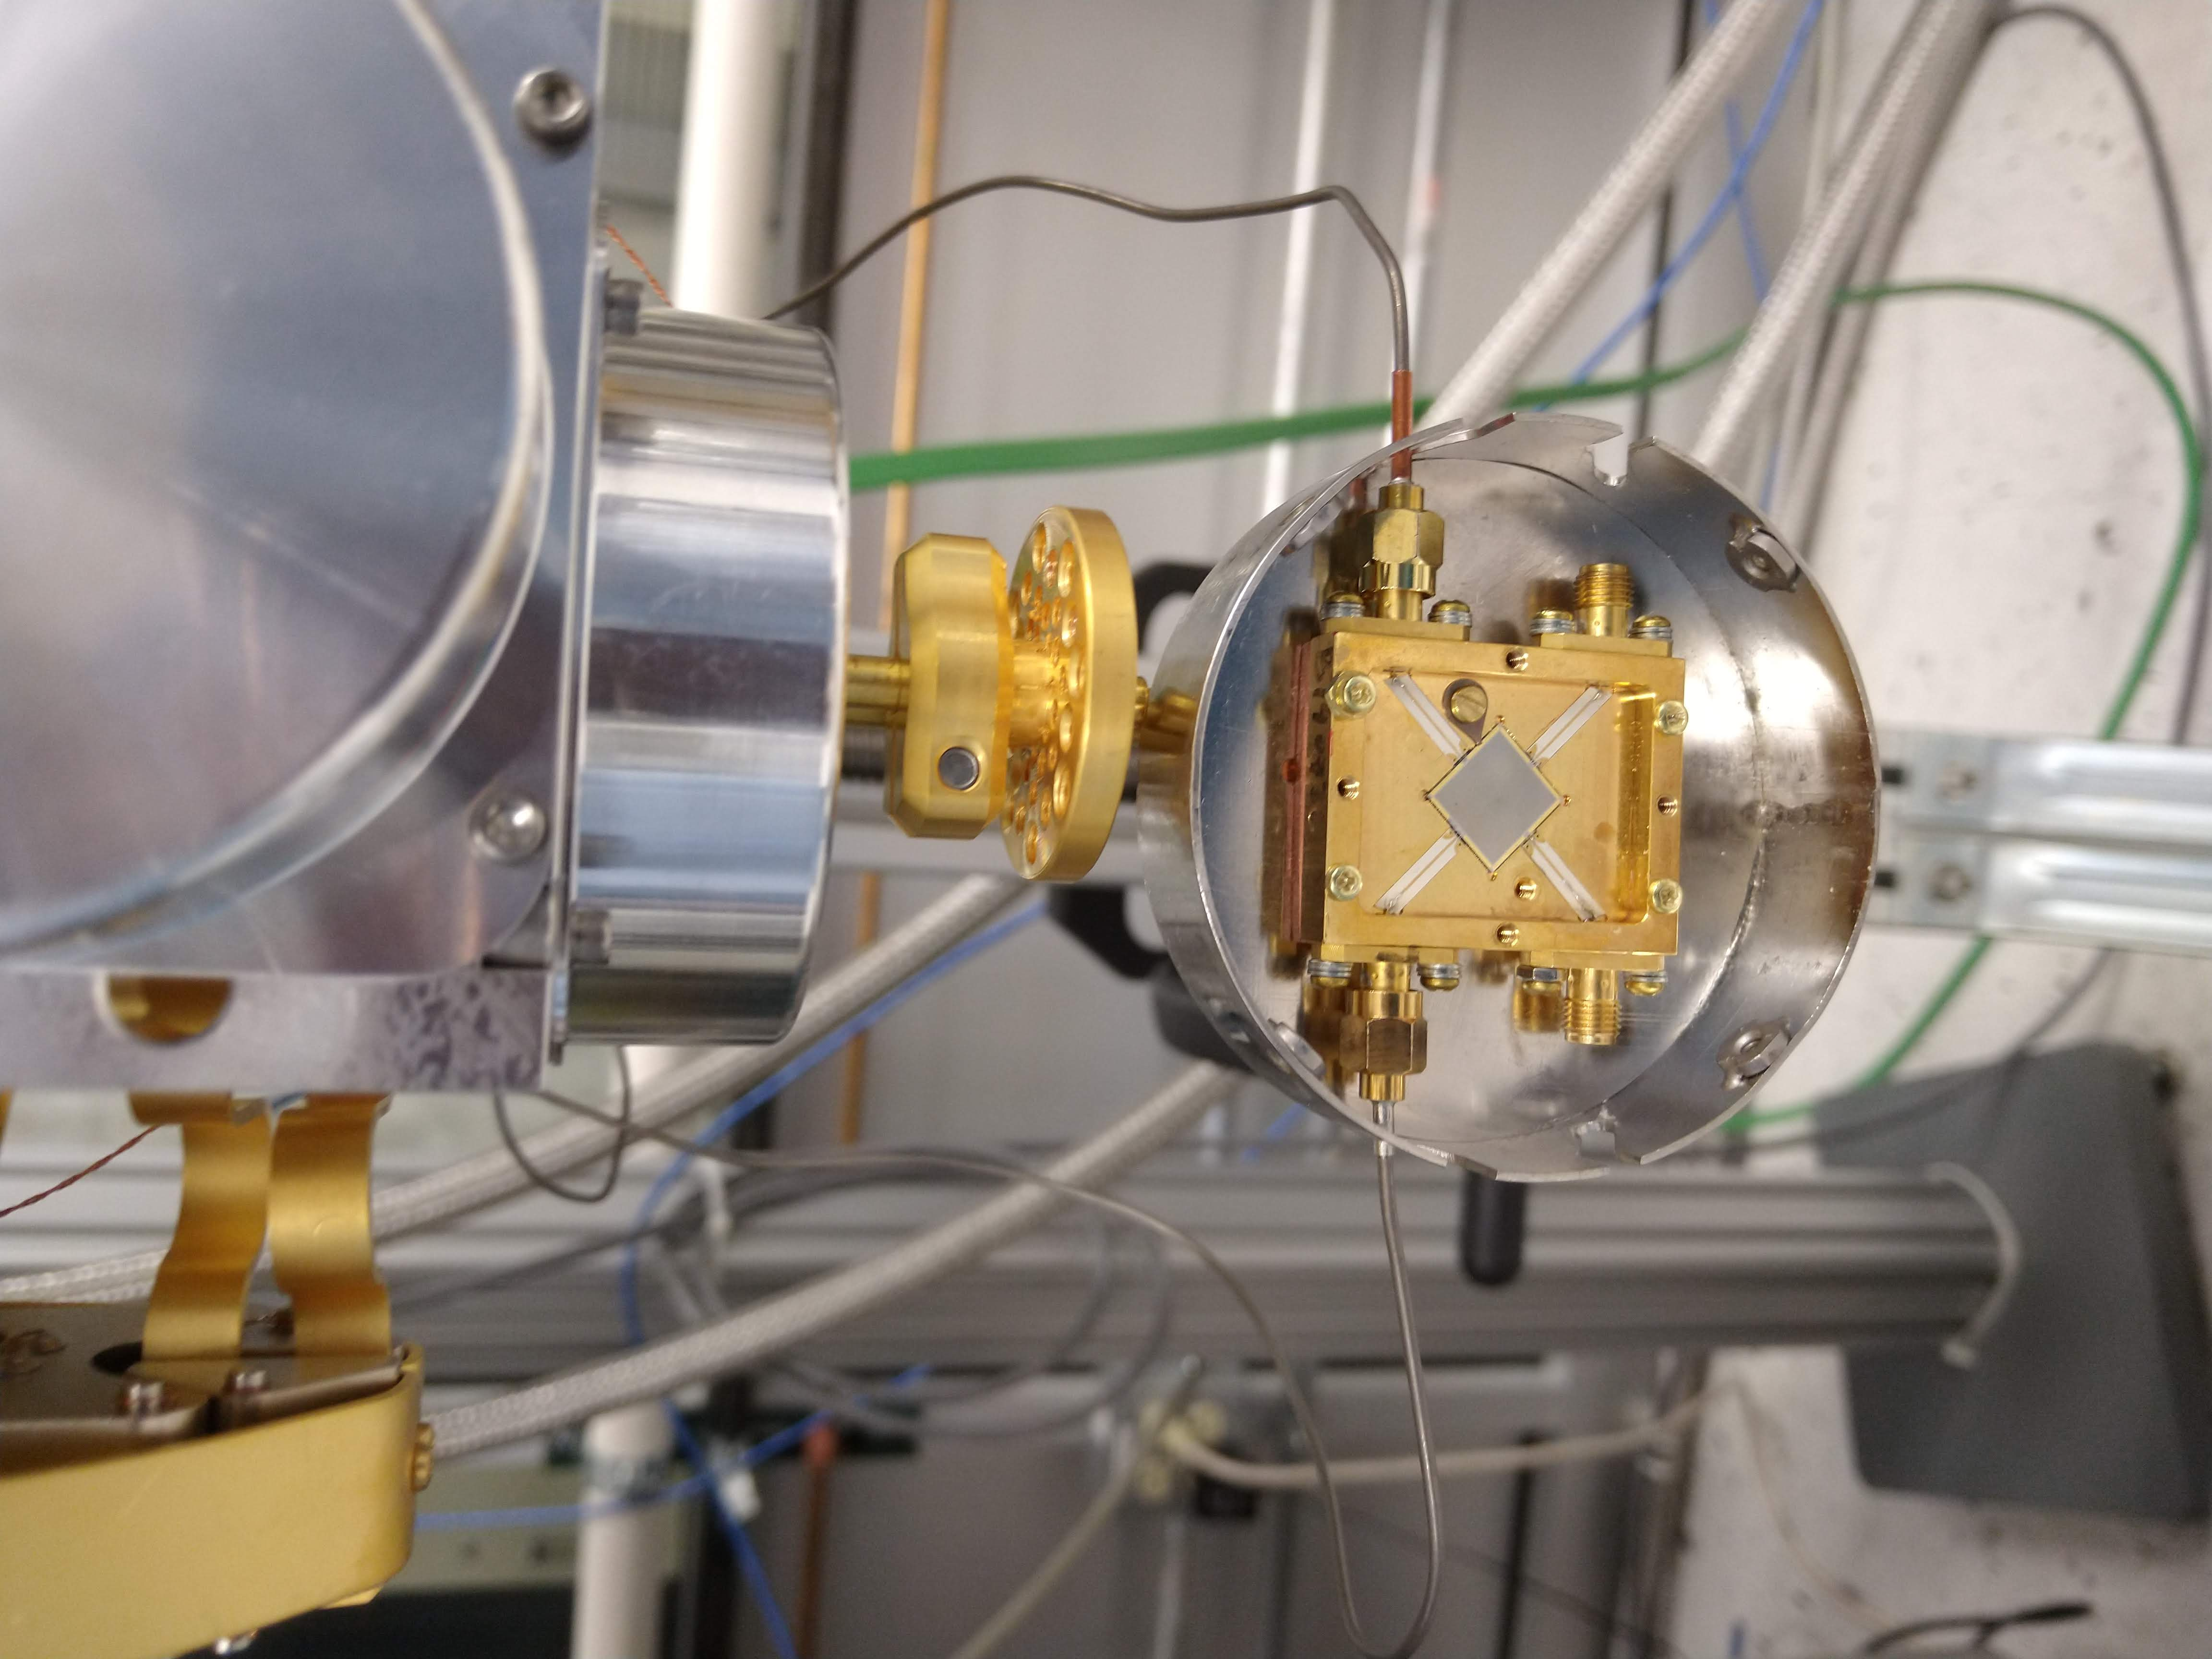
\includegraphics[angle=-90,width=0.6\textwidth]{mkid2}
								\end{column}
								\begin{column}{0.45\textwidth}
												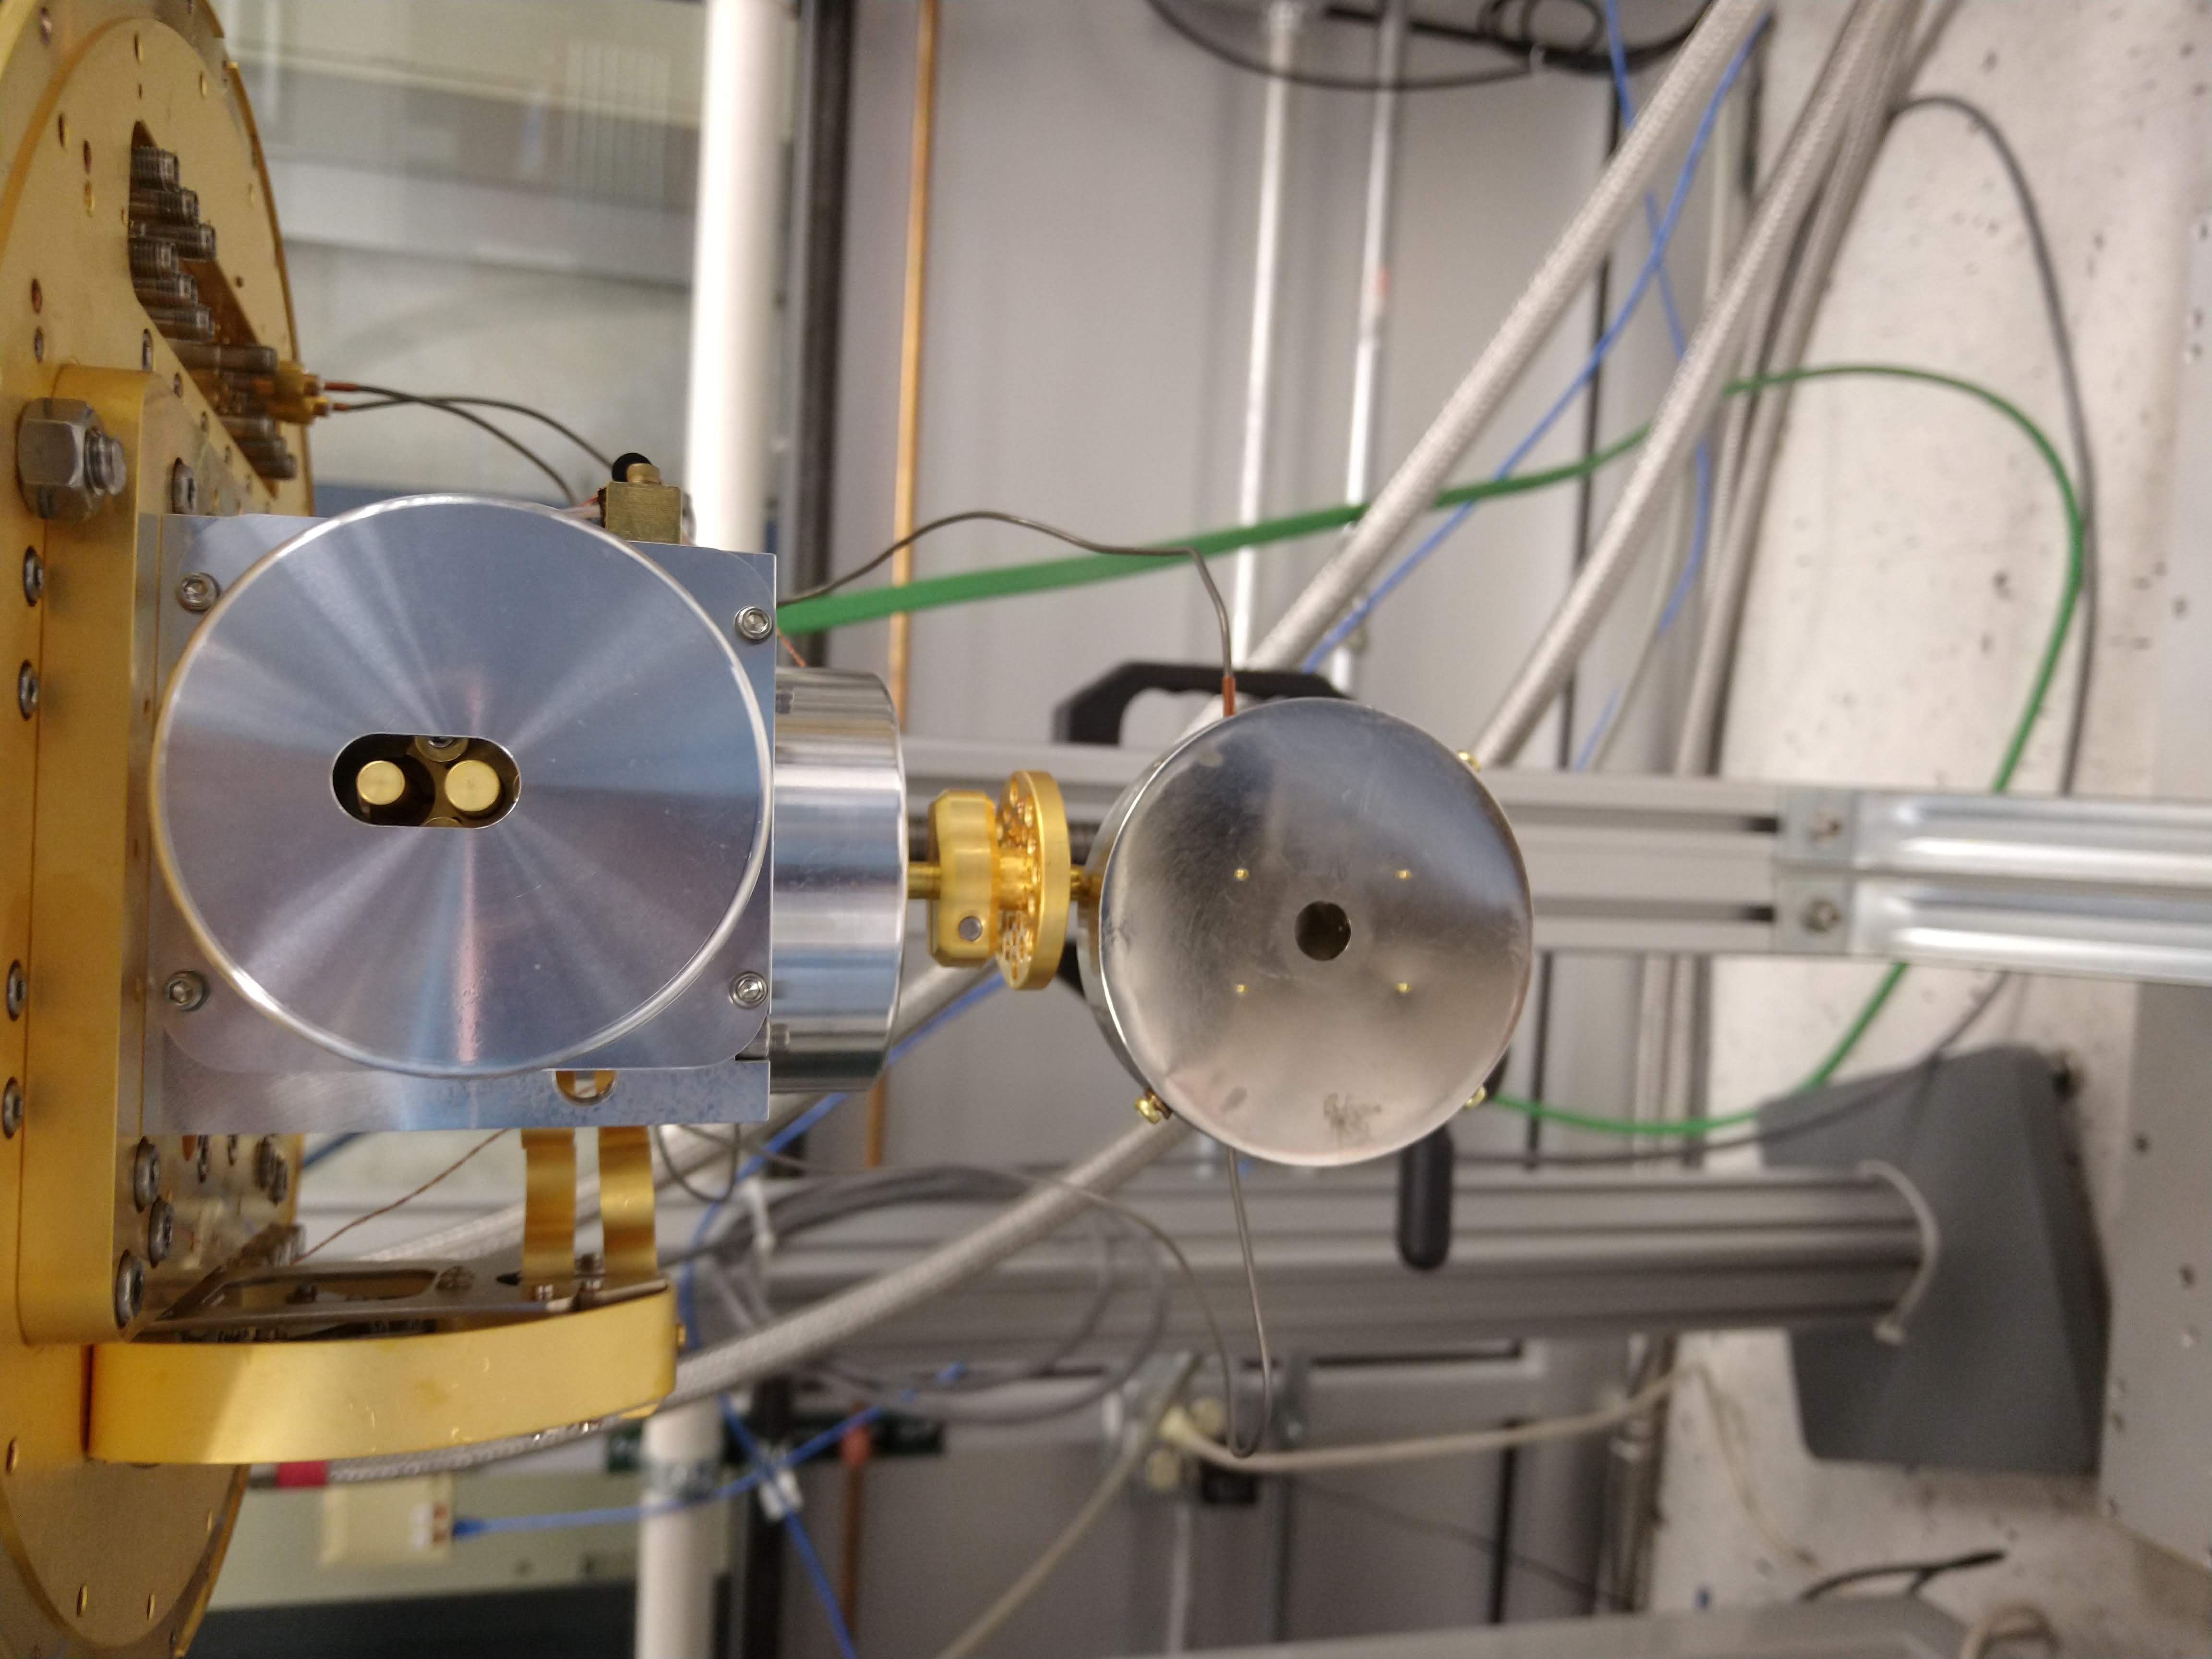
\includegraphics[angle=-90,width=0.62\textwidth]{mkid3_magnetic_case} \\ 
												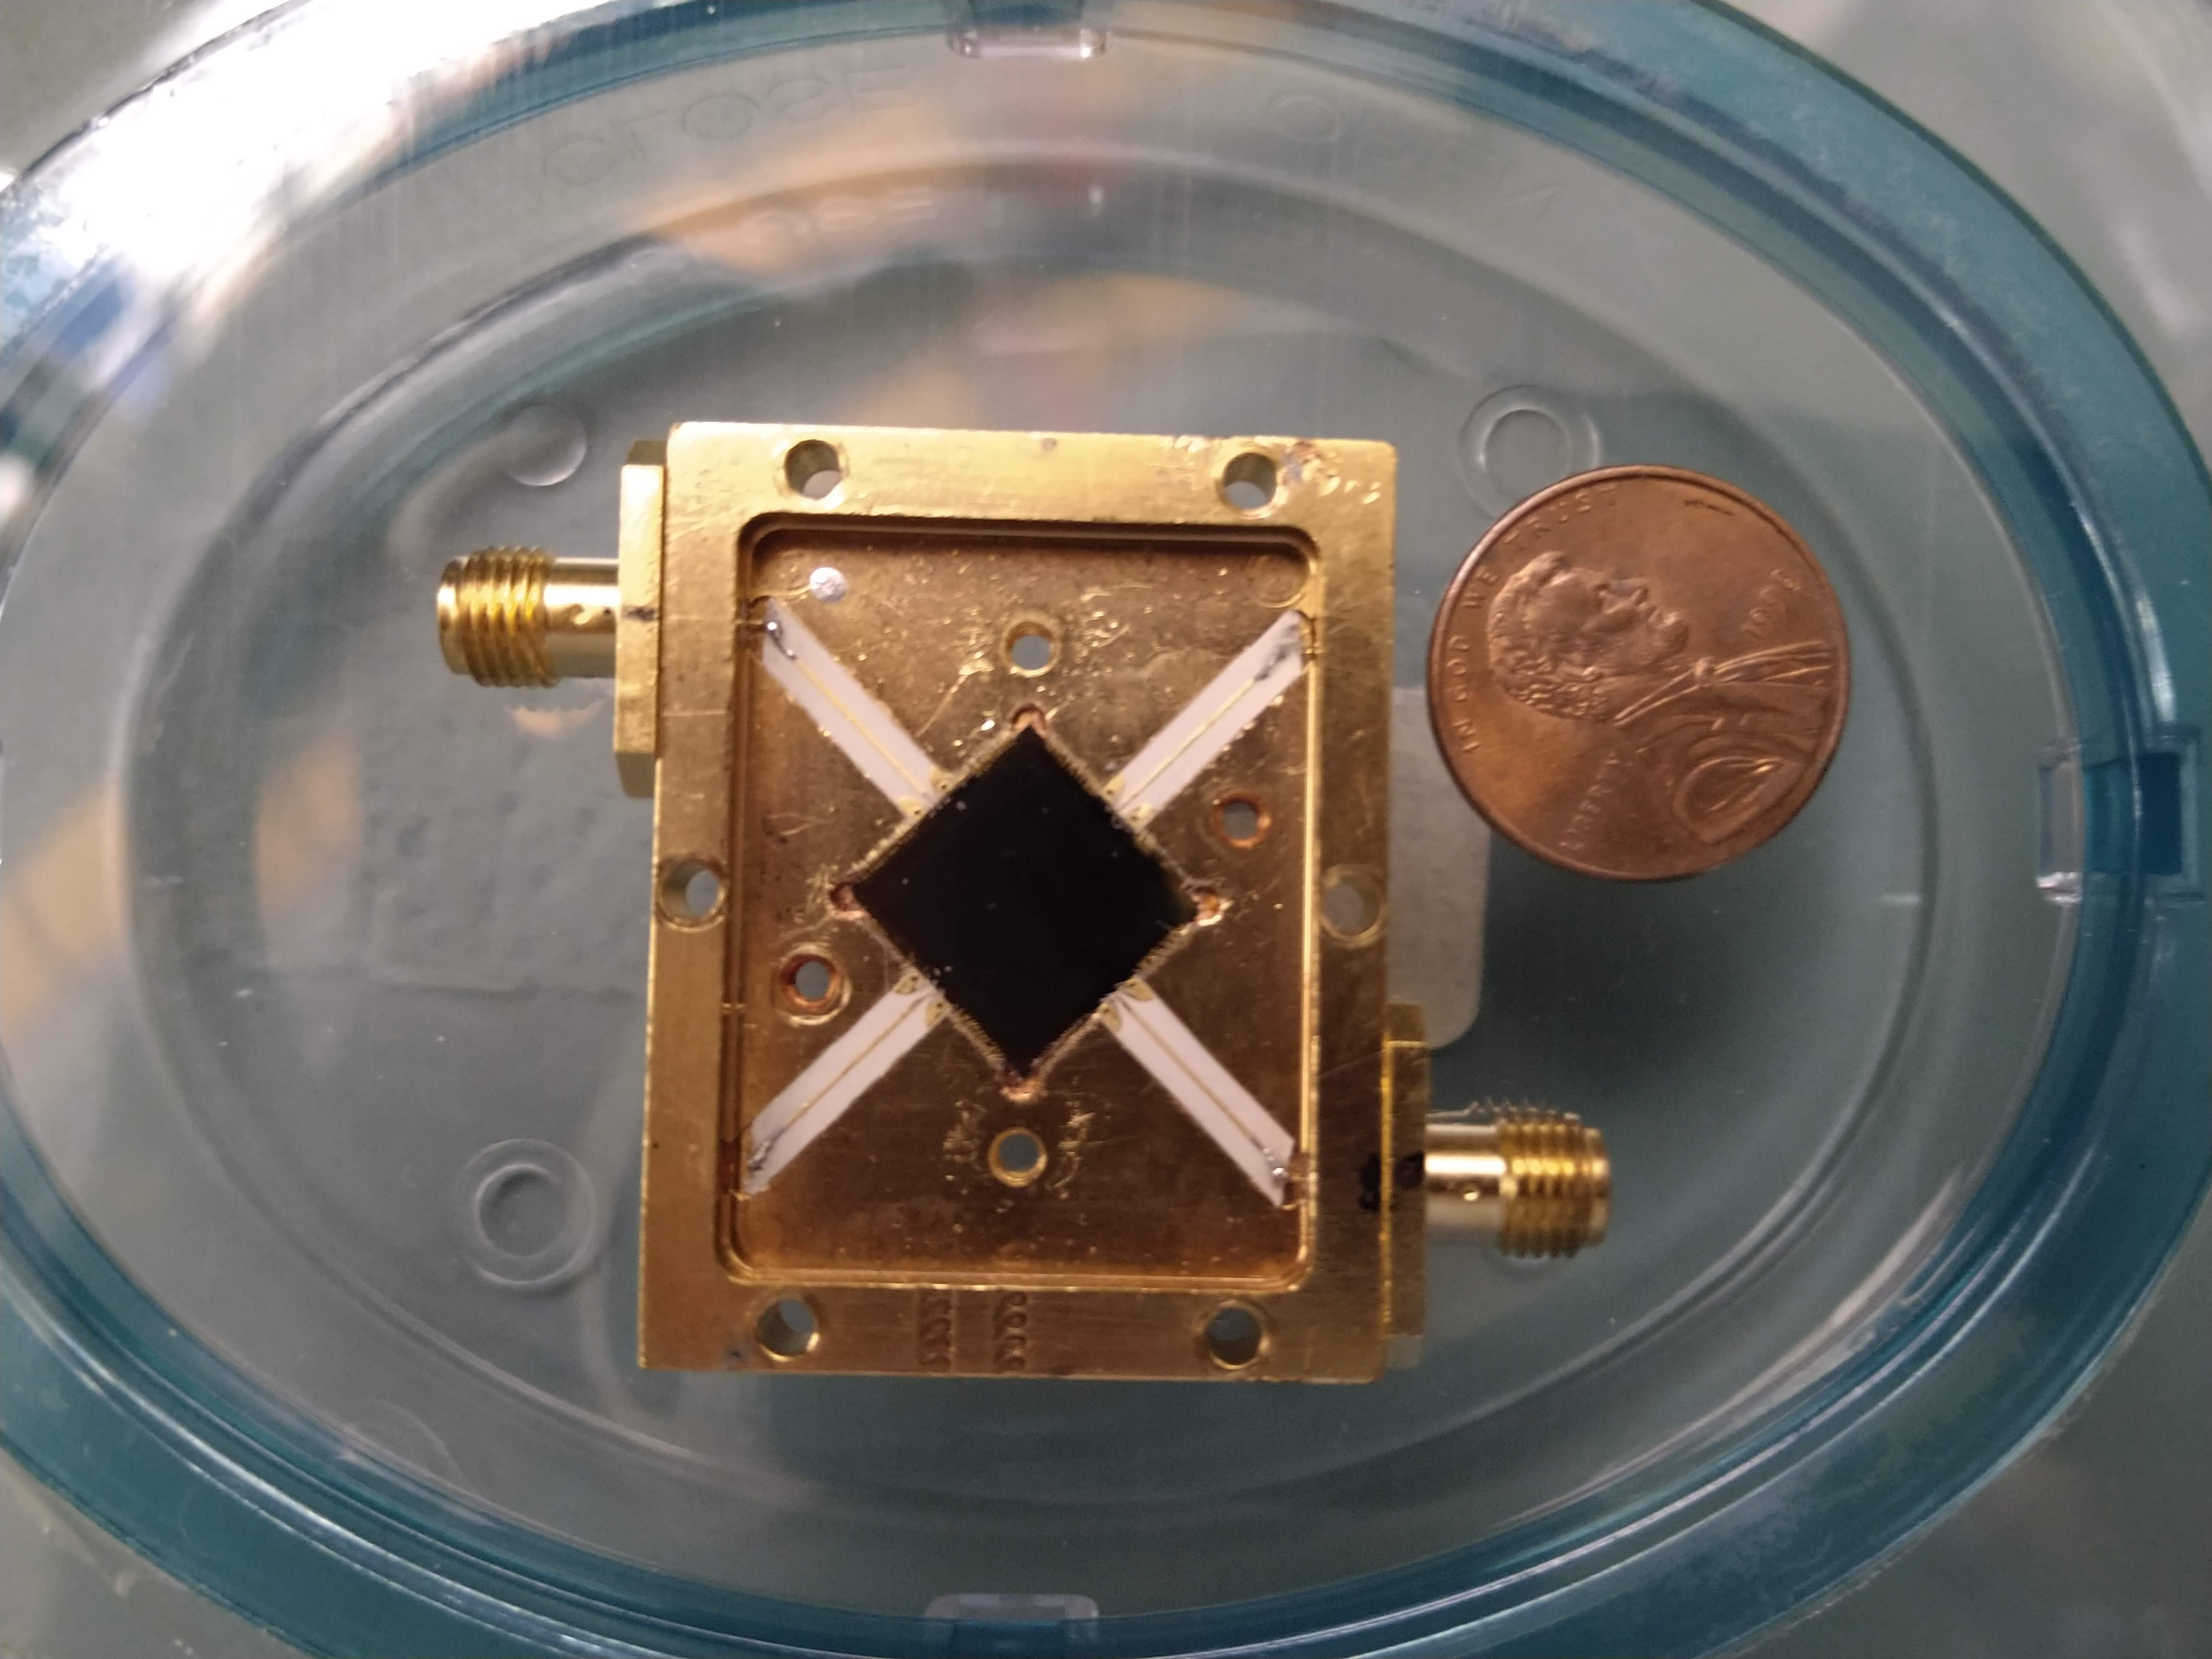
\includegraphics[angle=-90,width=0.6\textwidth]{mkid4}
								\end{column}
				\end{columns}
\end{frame}

\section{Amplificador de bajo ruido}
\begin{frame}{Amplificador}
				\begin{columns}
								\begin{column}{0.45\textwidth}
												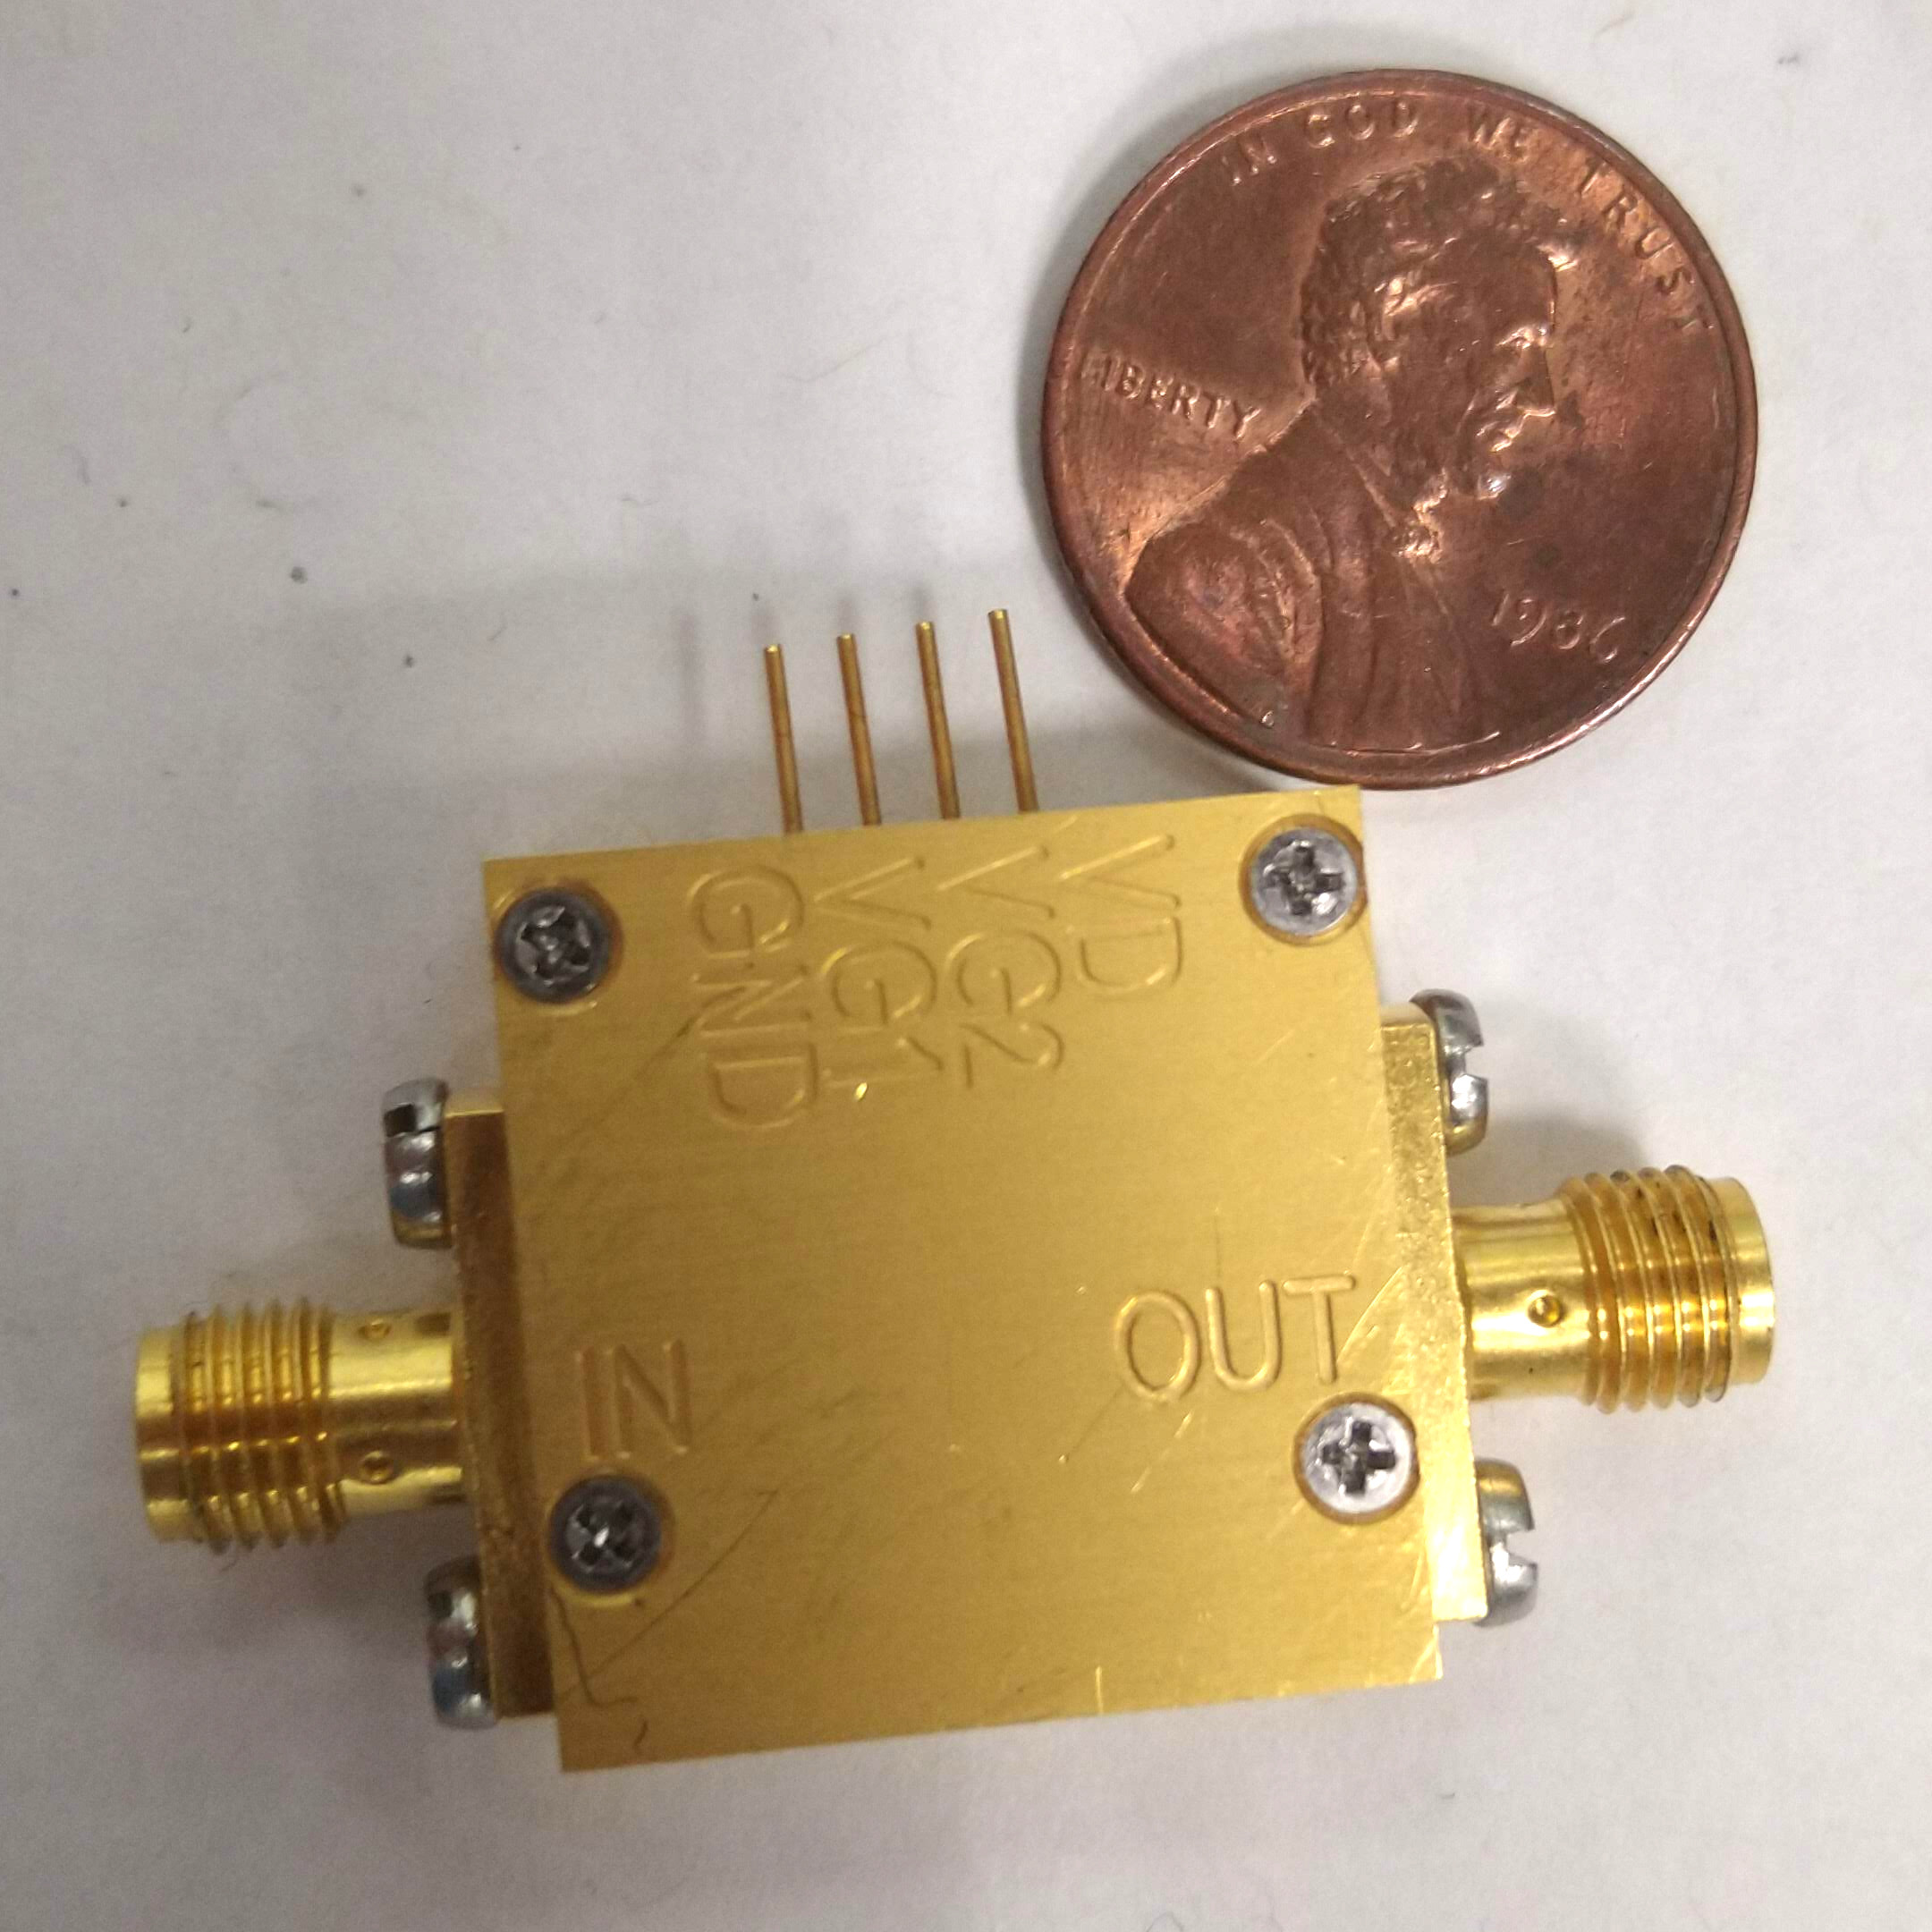
\includegraphics[angle=-90,width=0.62\textwidth]{amp_low_temp1} \\ 
												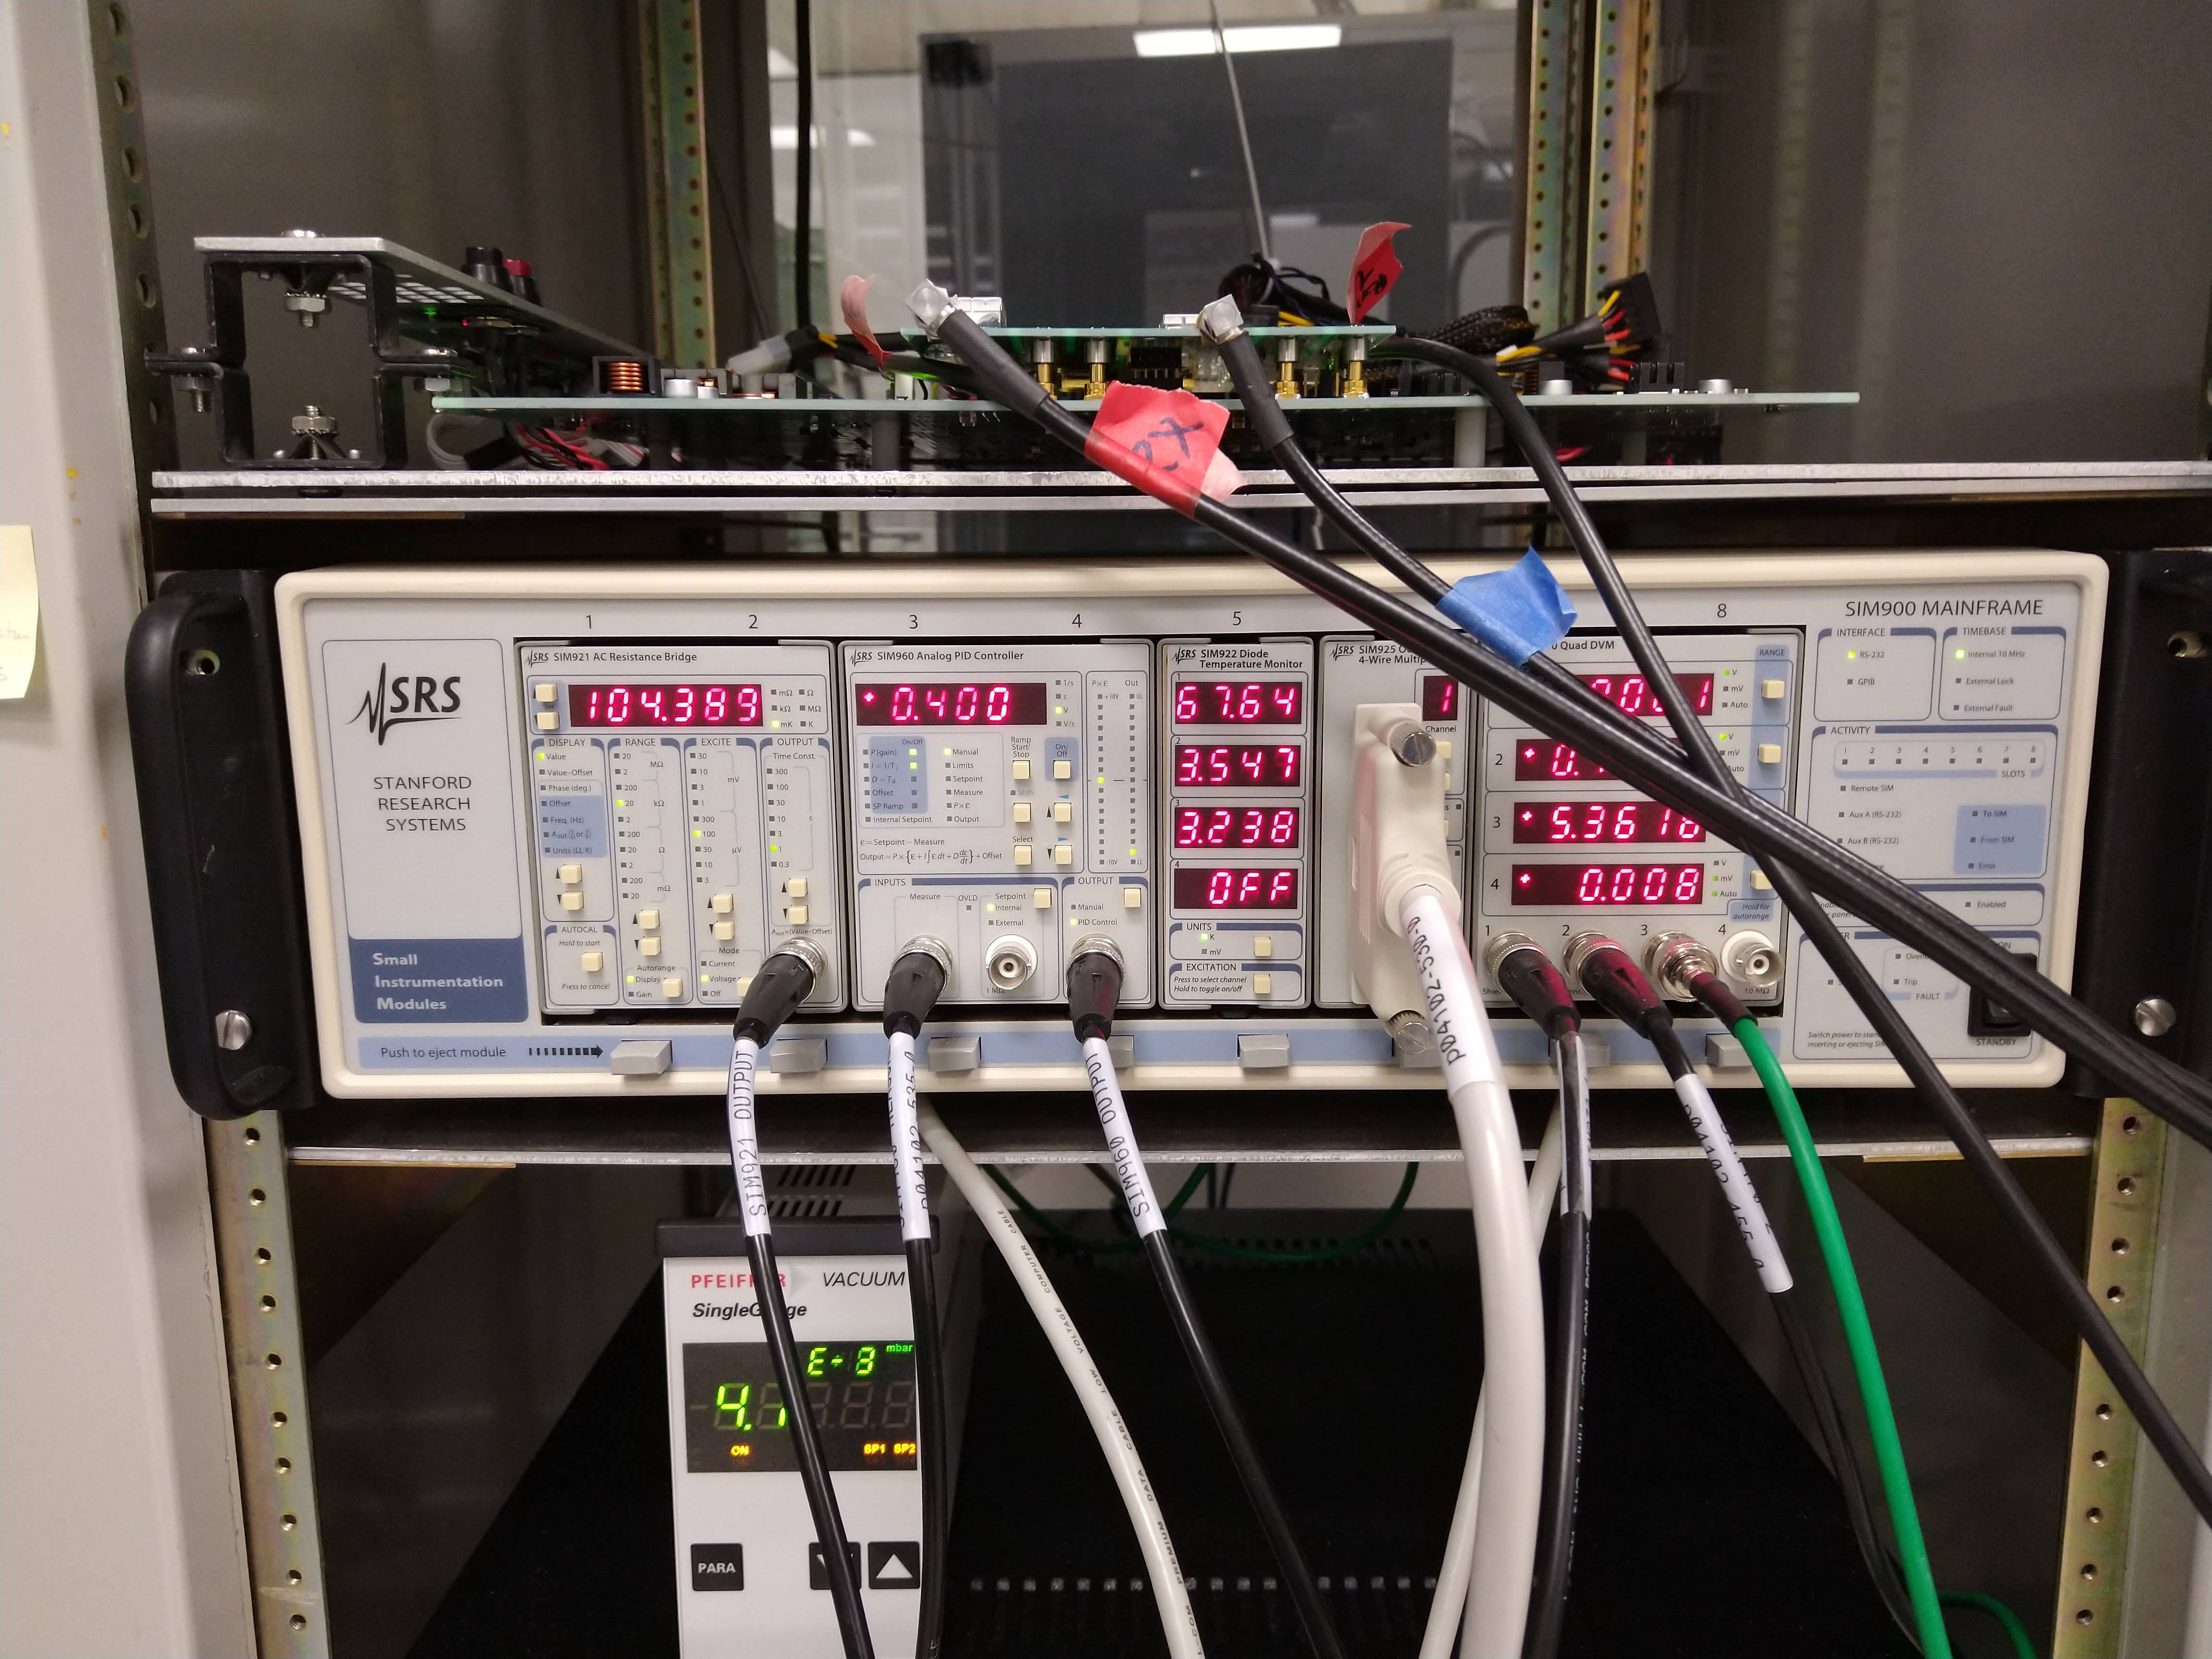
\includegraphics[angle=-90,width=0.6\textwidth]{sim900_mainframe_med_temp}
								\end{column}
								\begin{column}{0.45\textwidth}
												\includegraphics[angle=-90,width=0.62\textwidth]{acople_linea_mkid} \\ 
												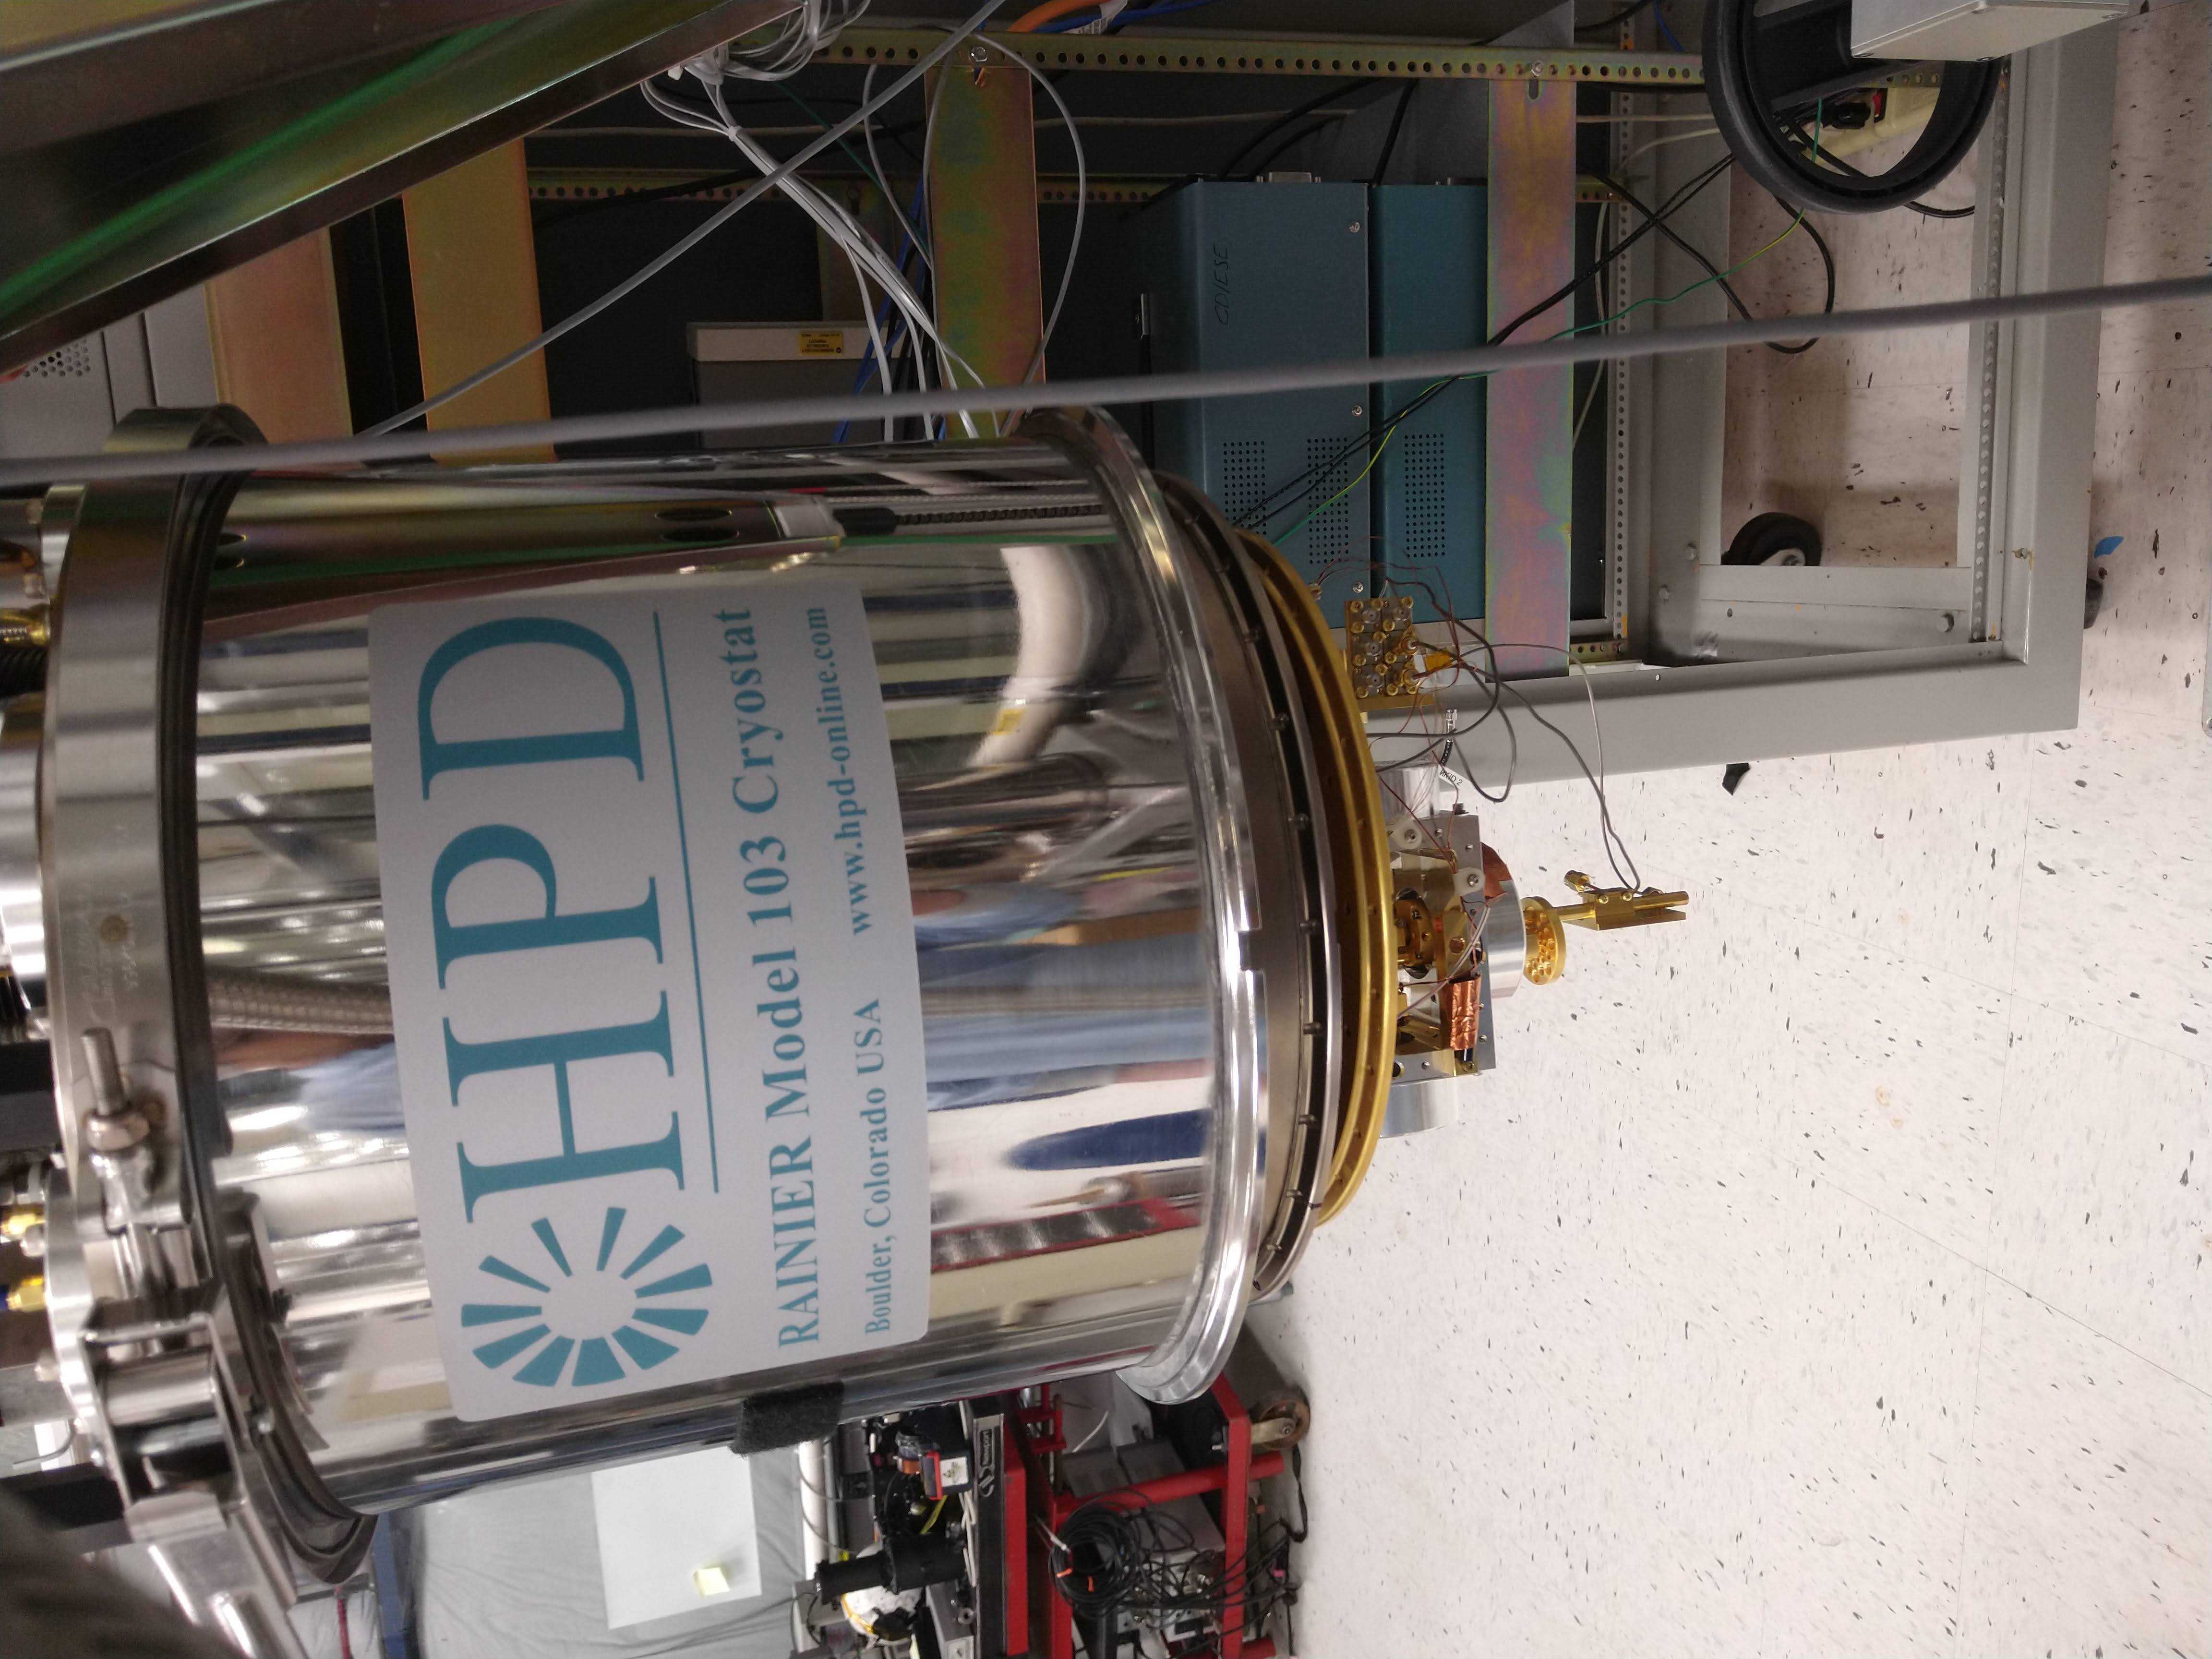
\includegraphics[angle=-90,width=0.6\textwidth]{criostato_modelo}
								\end{column}
				\end{columns}
\end{frame}
\section{Equipamiento BT}
Using section and subsection commands, outside of frames, provides a table of contents and progress information to beamer.
\begin{frame}{Equipos BT}
				\begin{columns}
								\begin{column}{0.45\textwidth}
												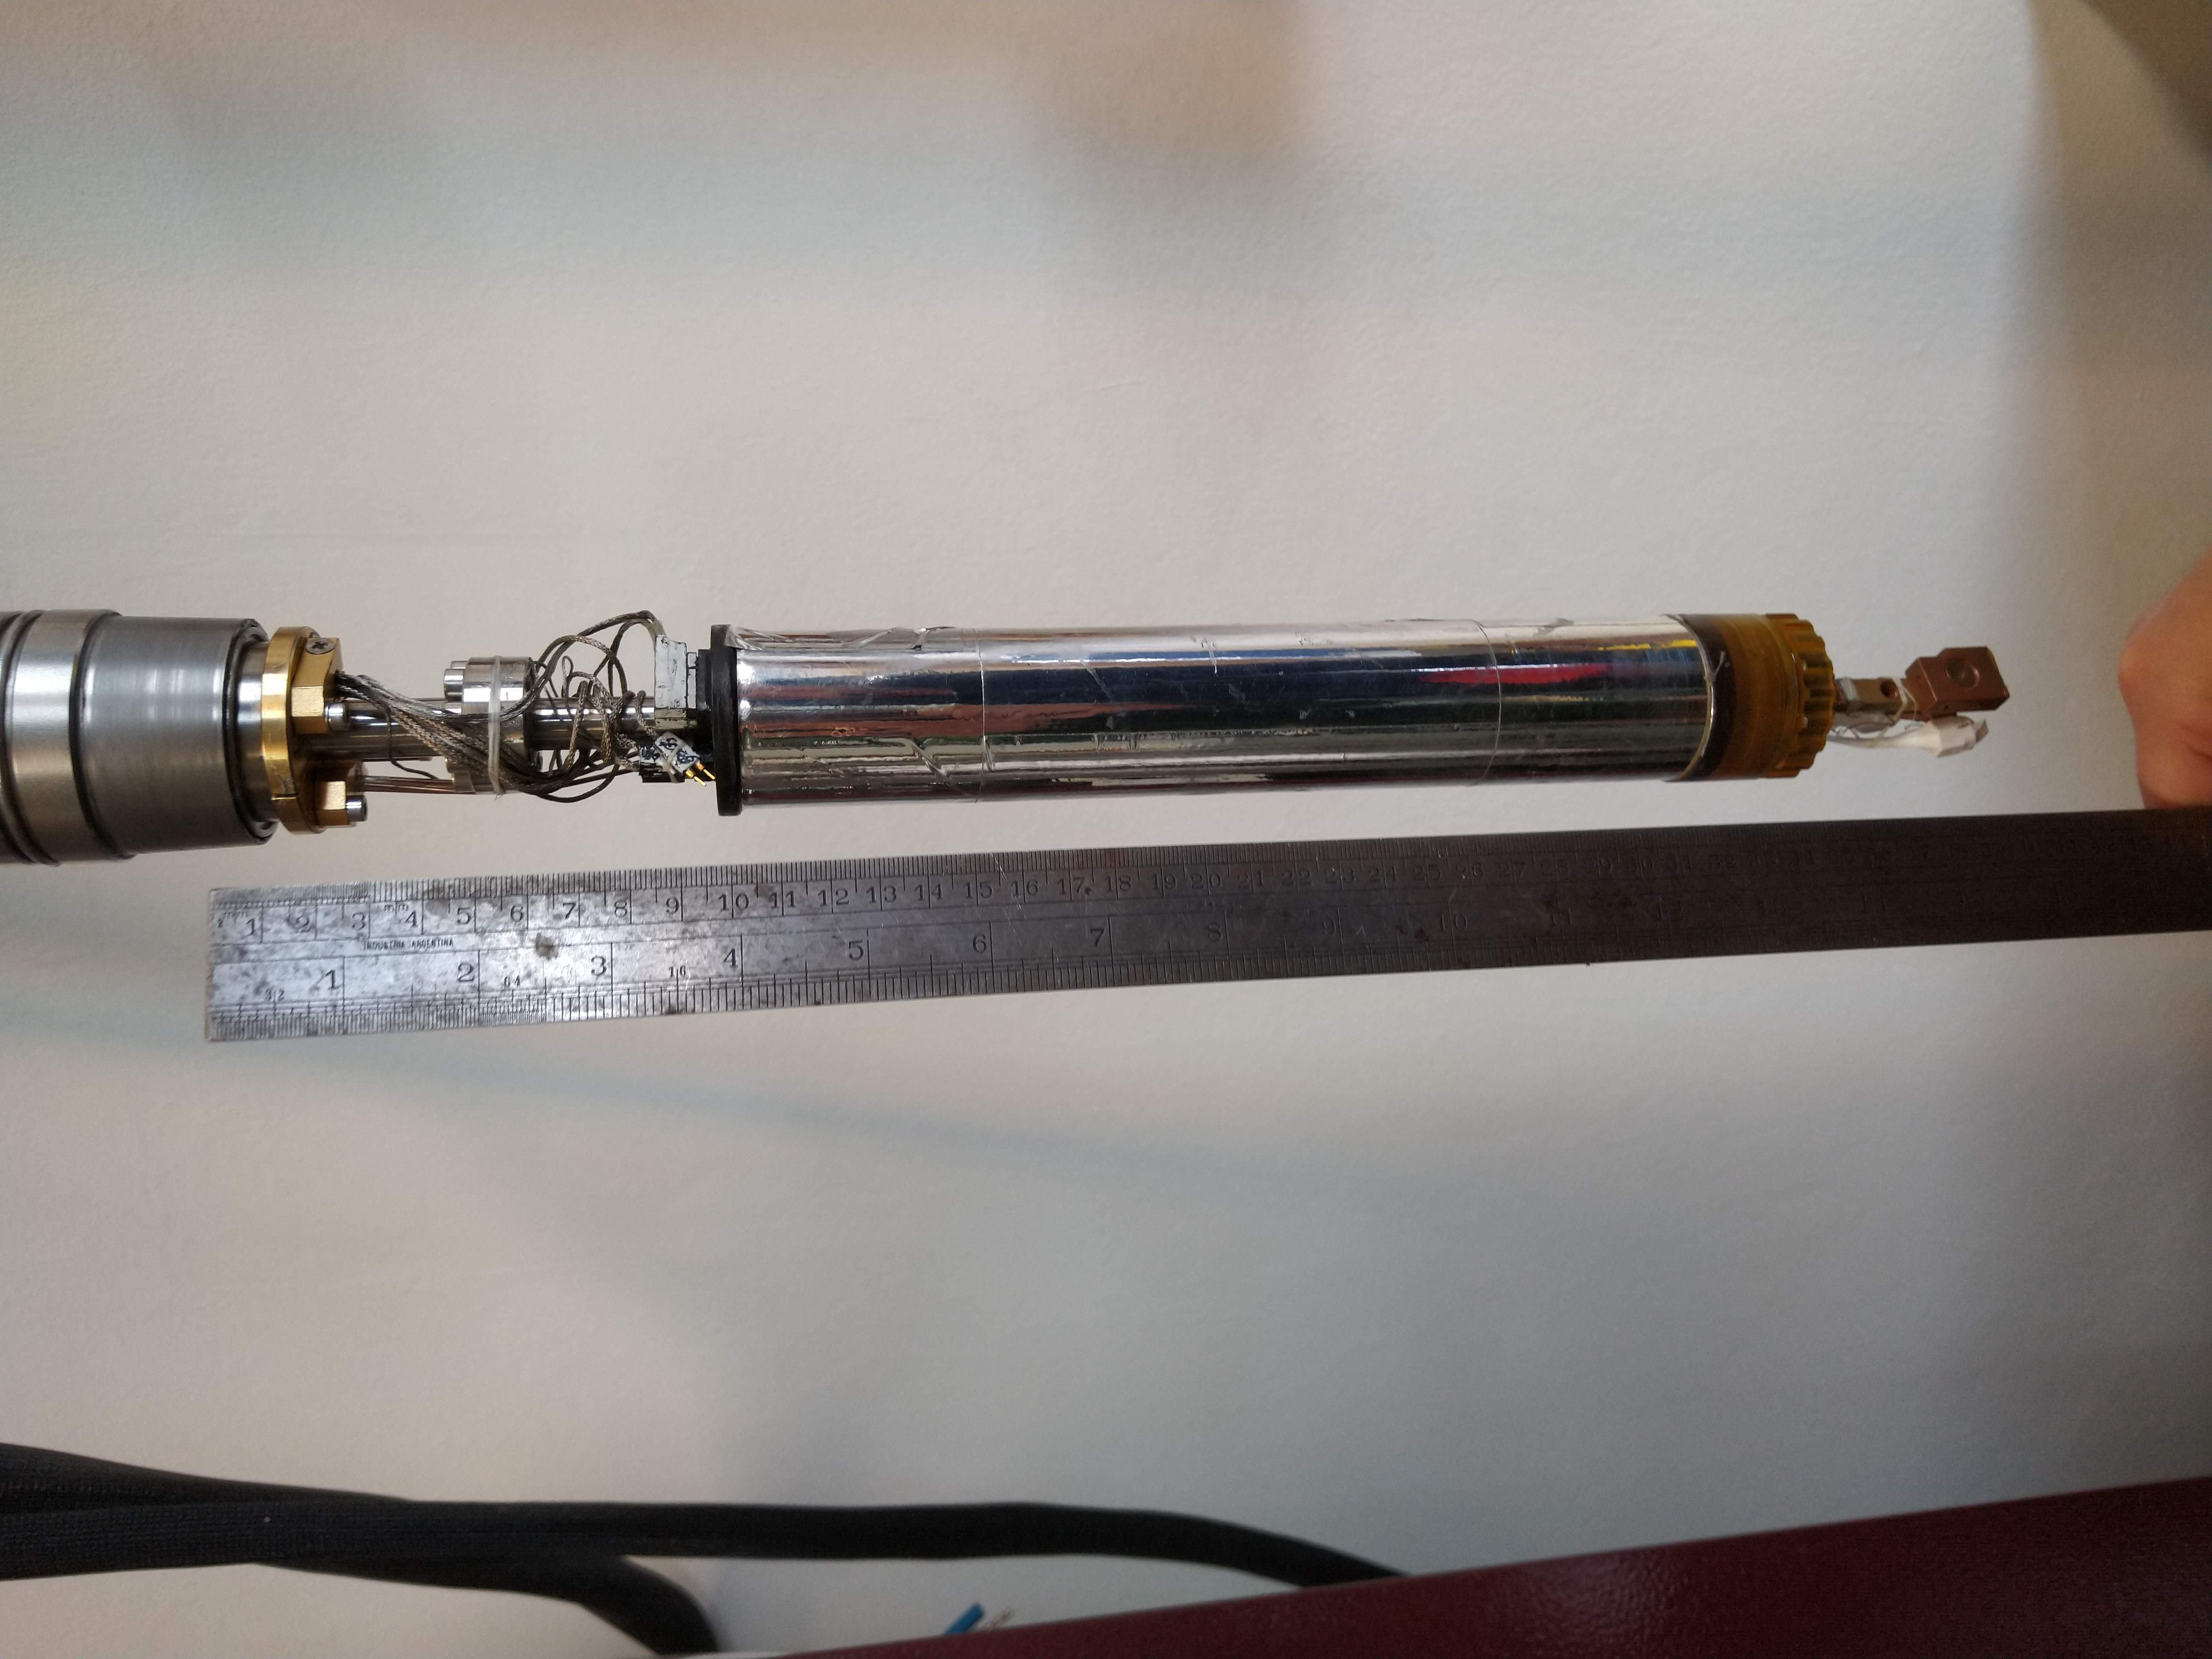
\includegraphics[angle=-90,width=0.62\textwidth]{IMG_20190523_105037648} \\ 
												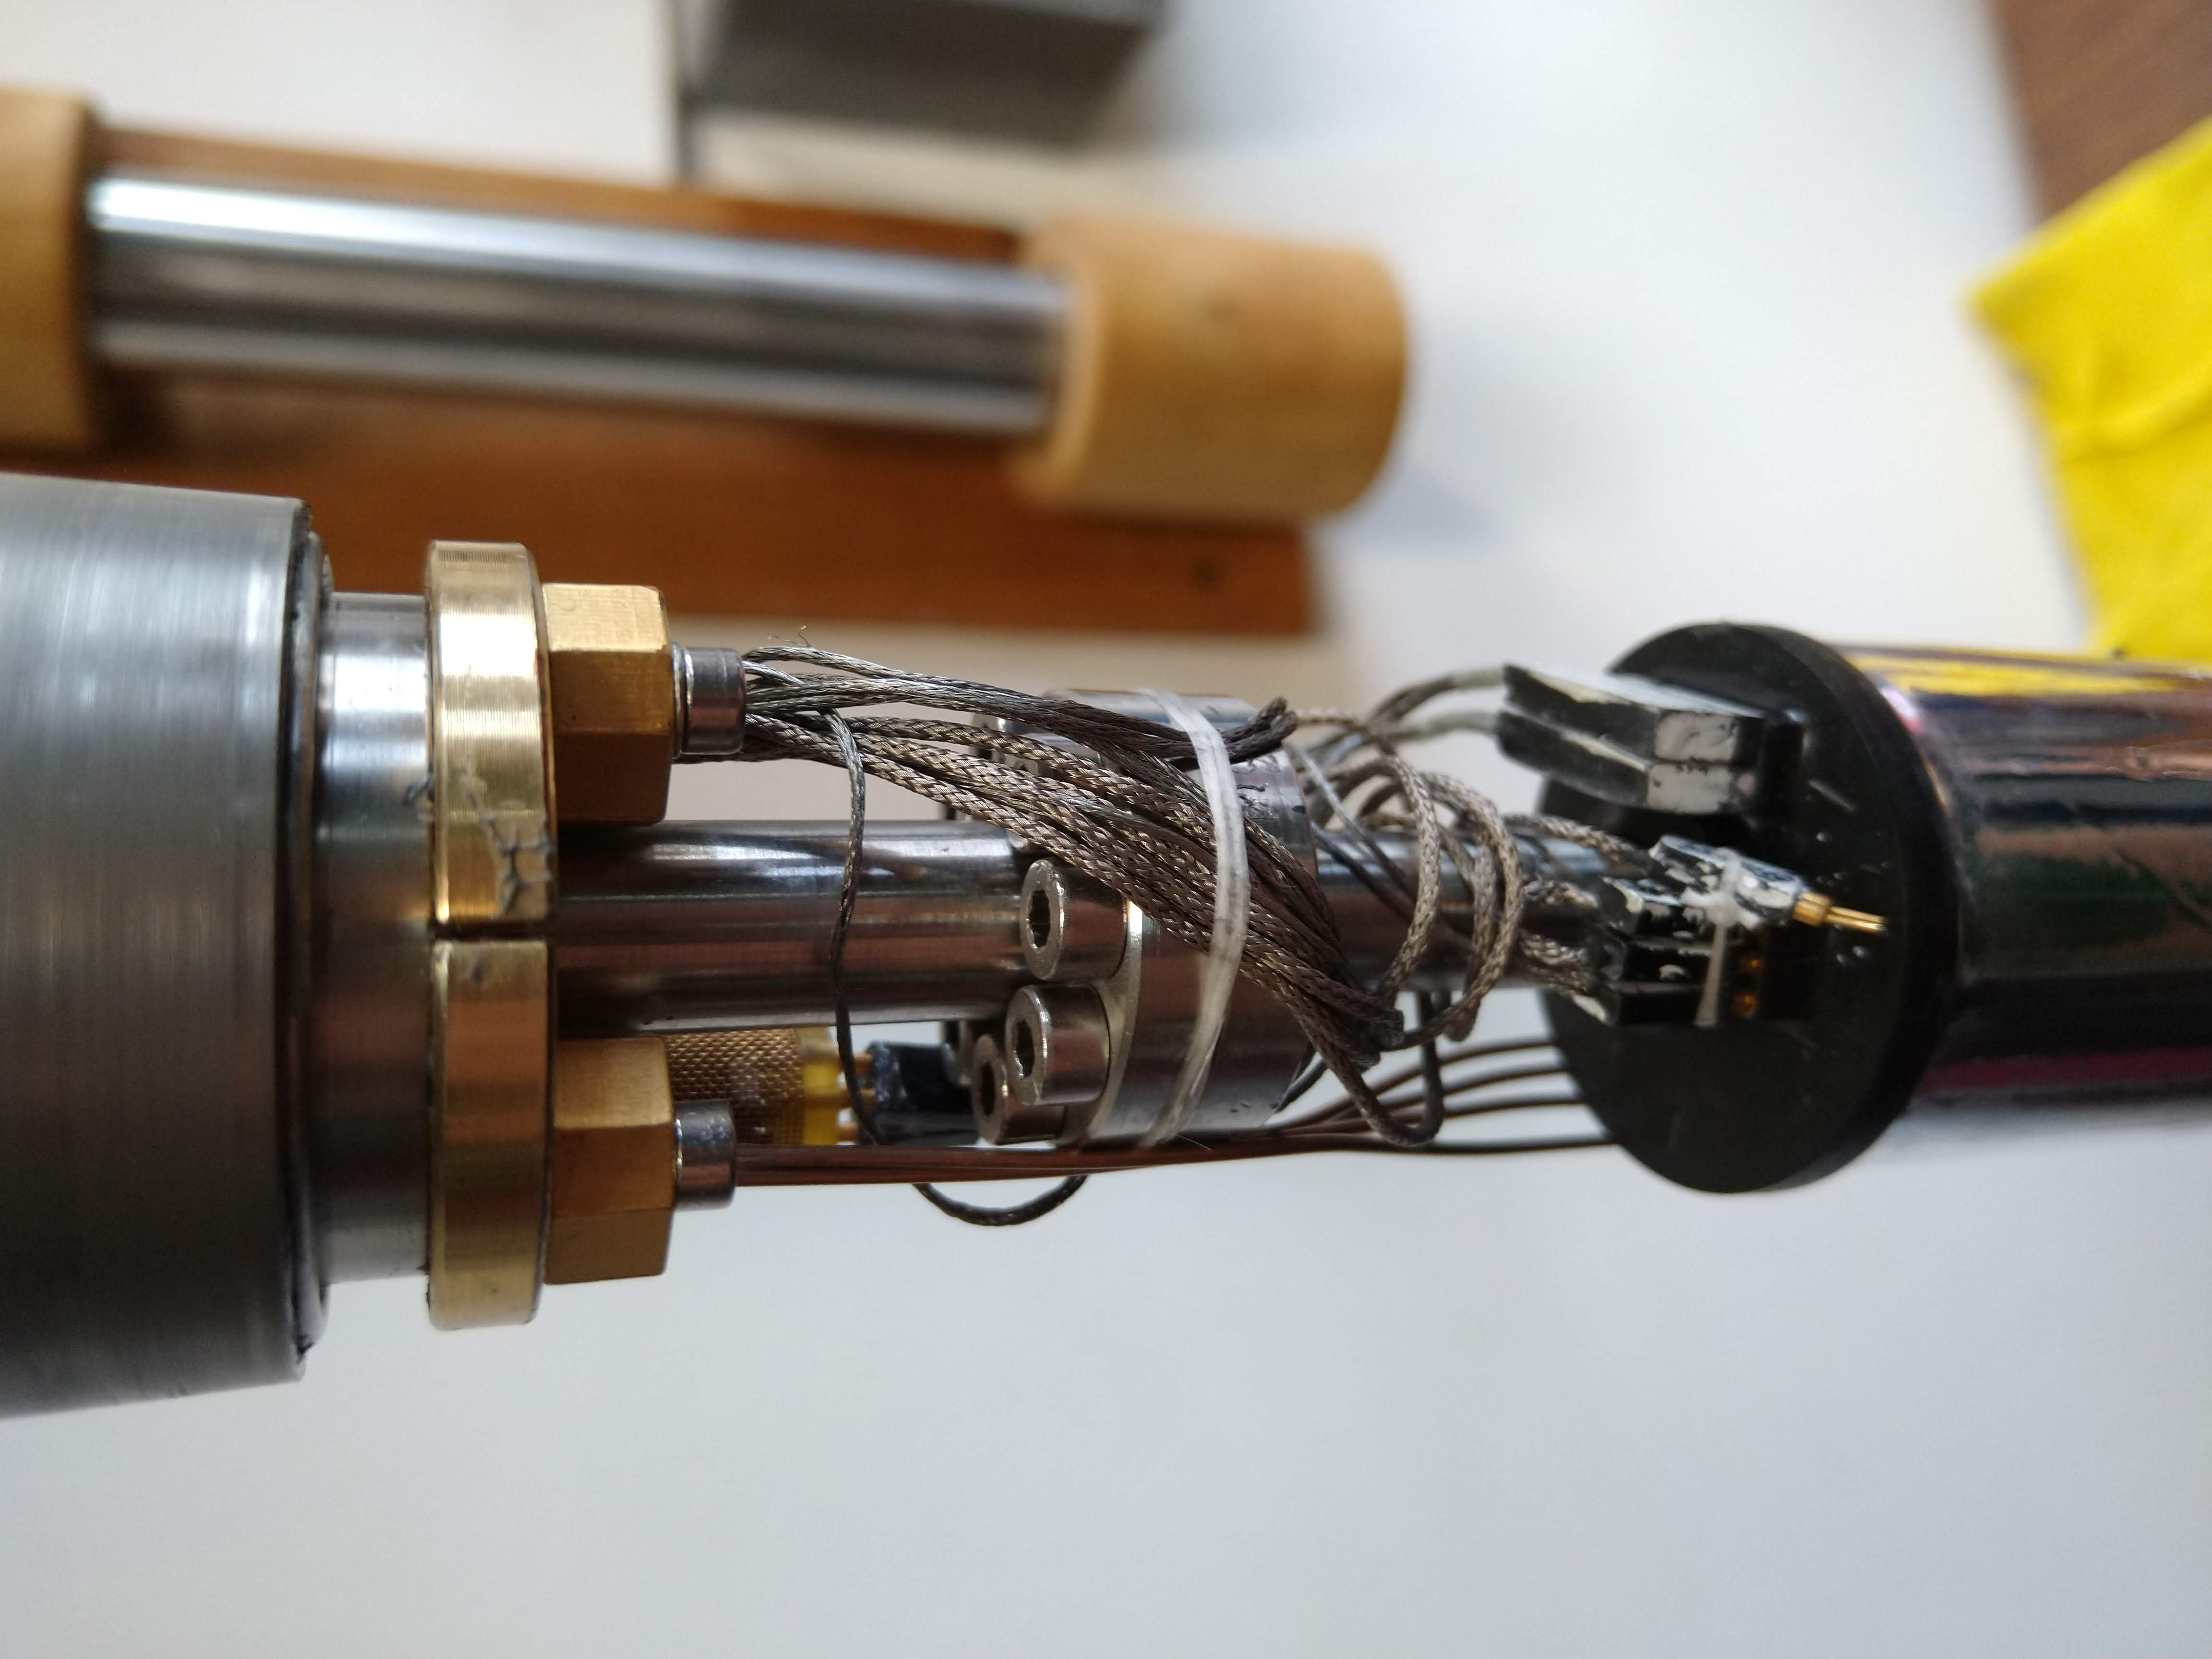
\includegraphics[angle=-90,width=0.6\textwidth]{IMG_20190523_105054061}
								\end{column}
								\begin{column}{0.45\textwidth}
												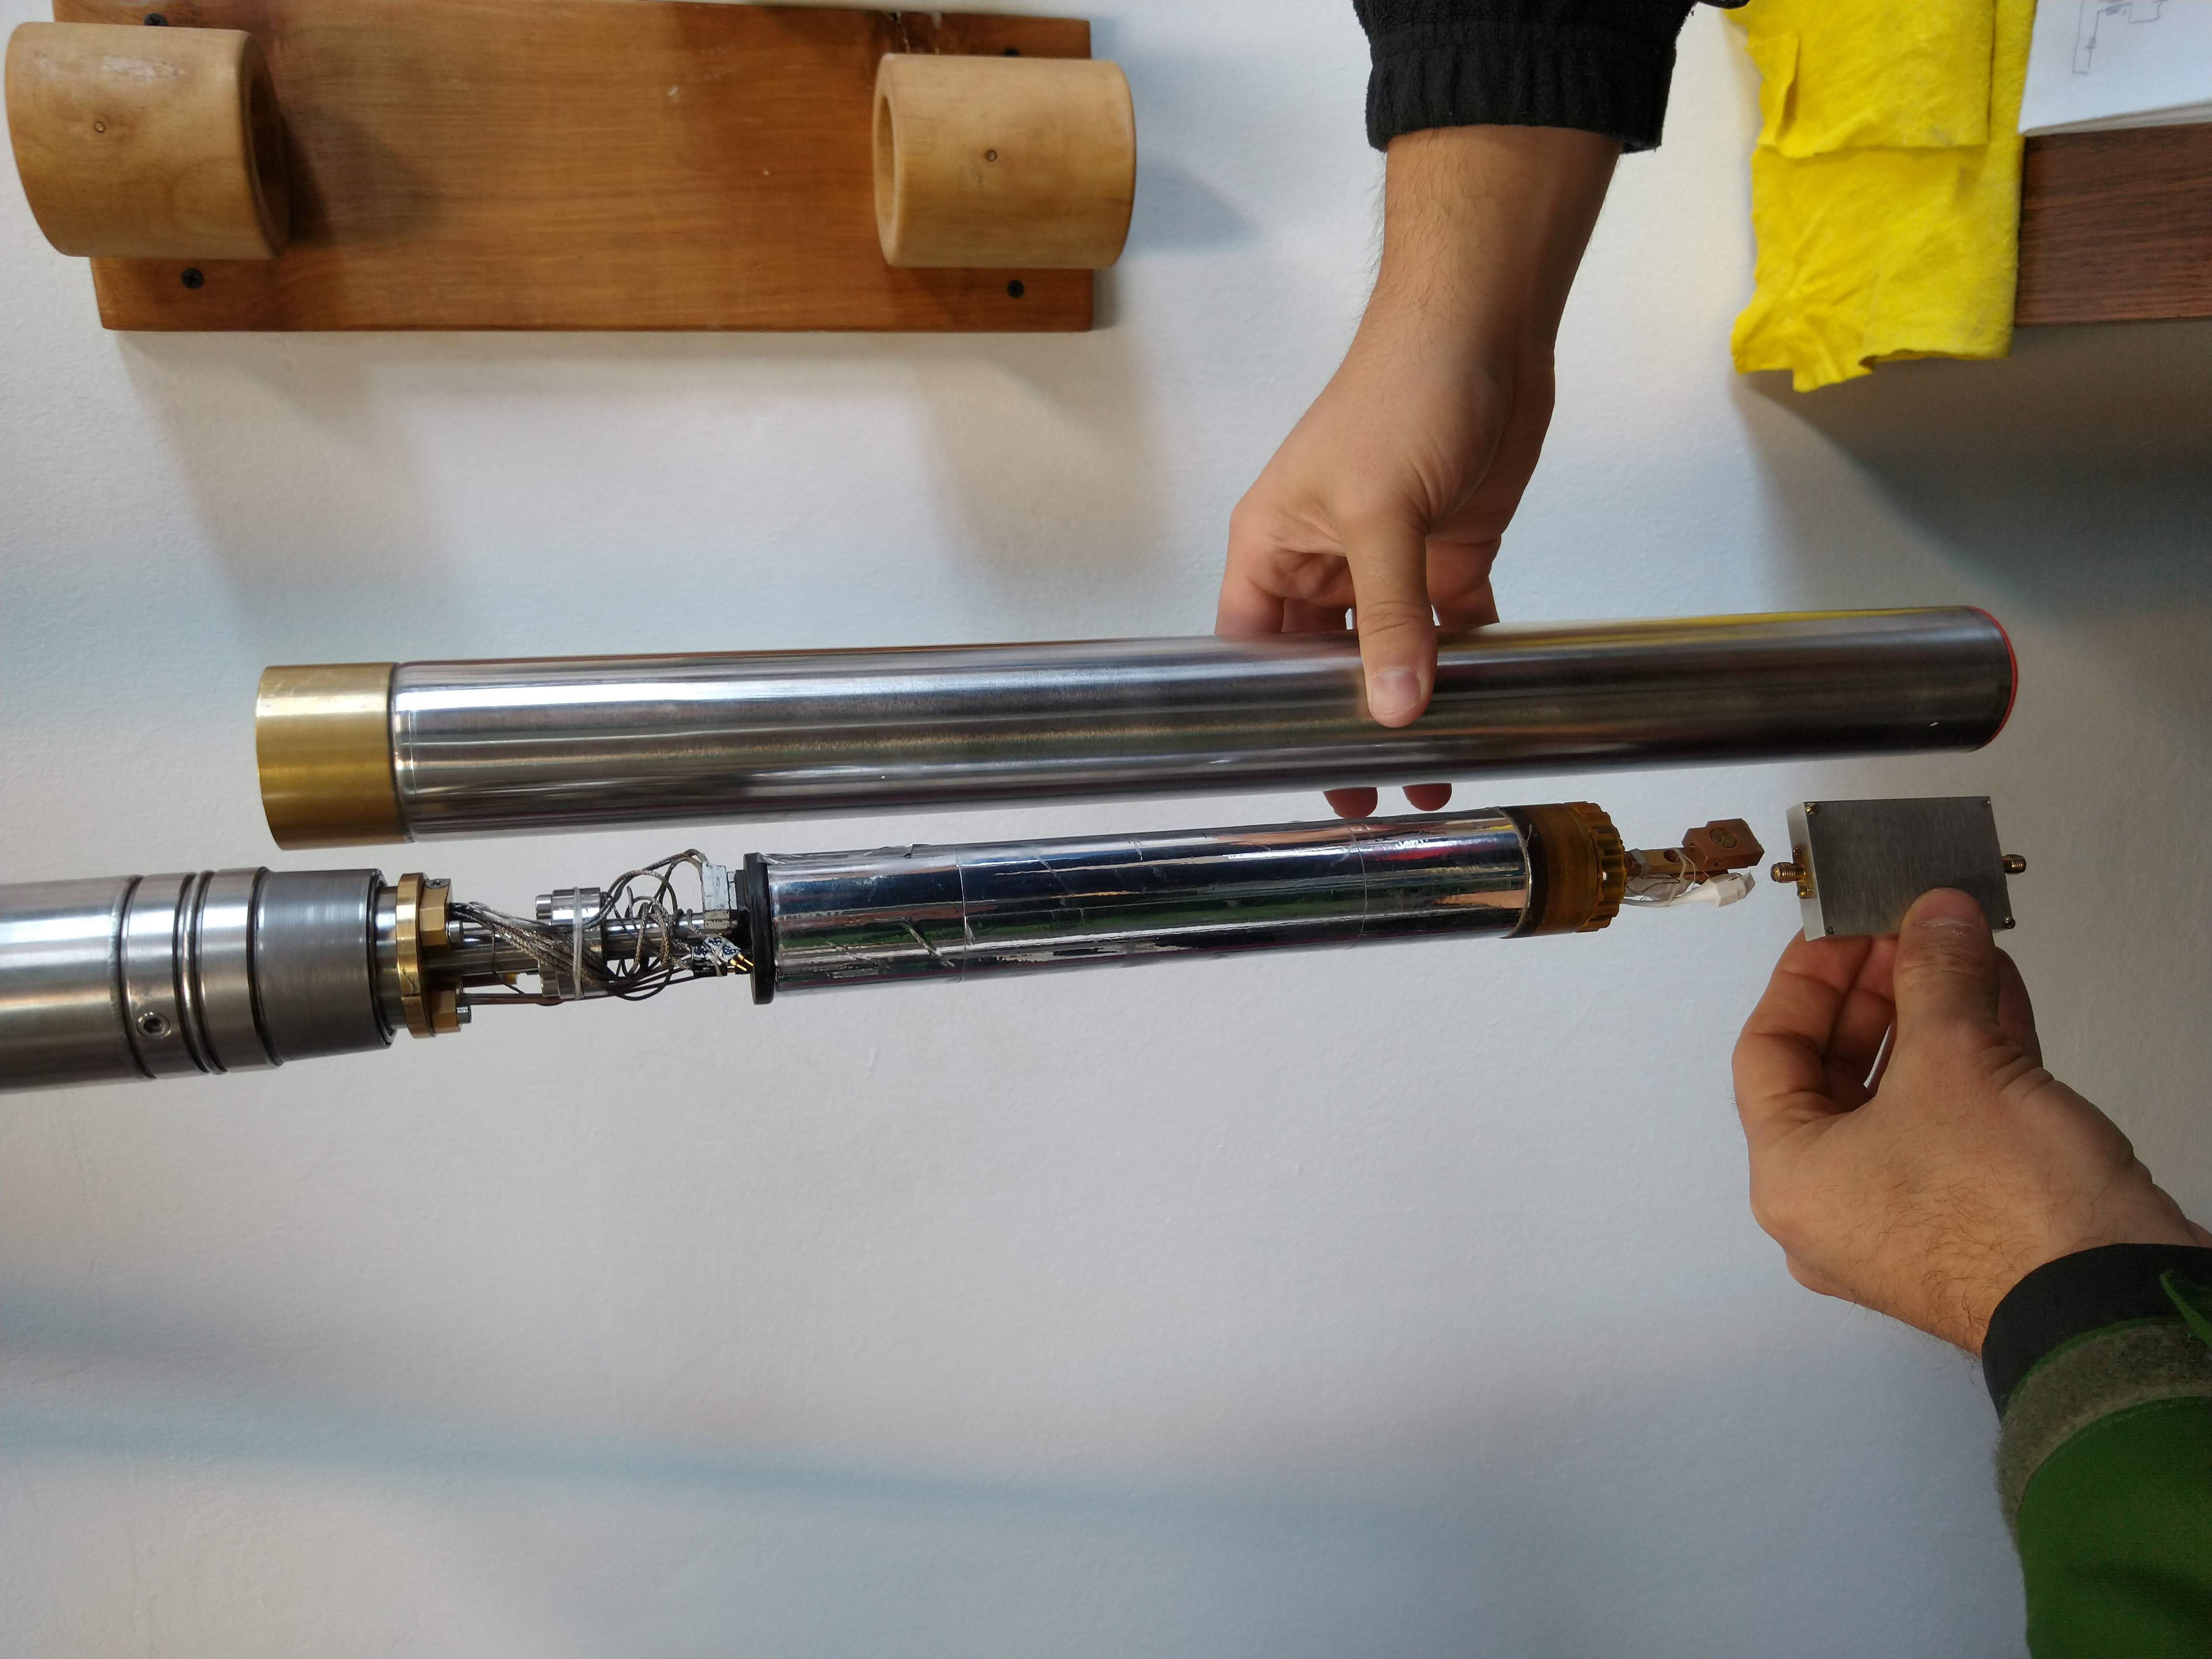
\includegraphics[angle=-90, width=0.62\textwidth]{IMG_20190523_105443289} \\ 
												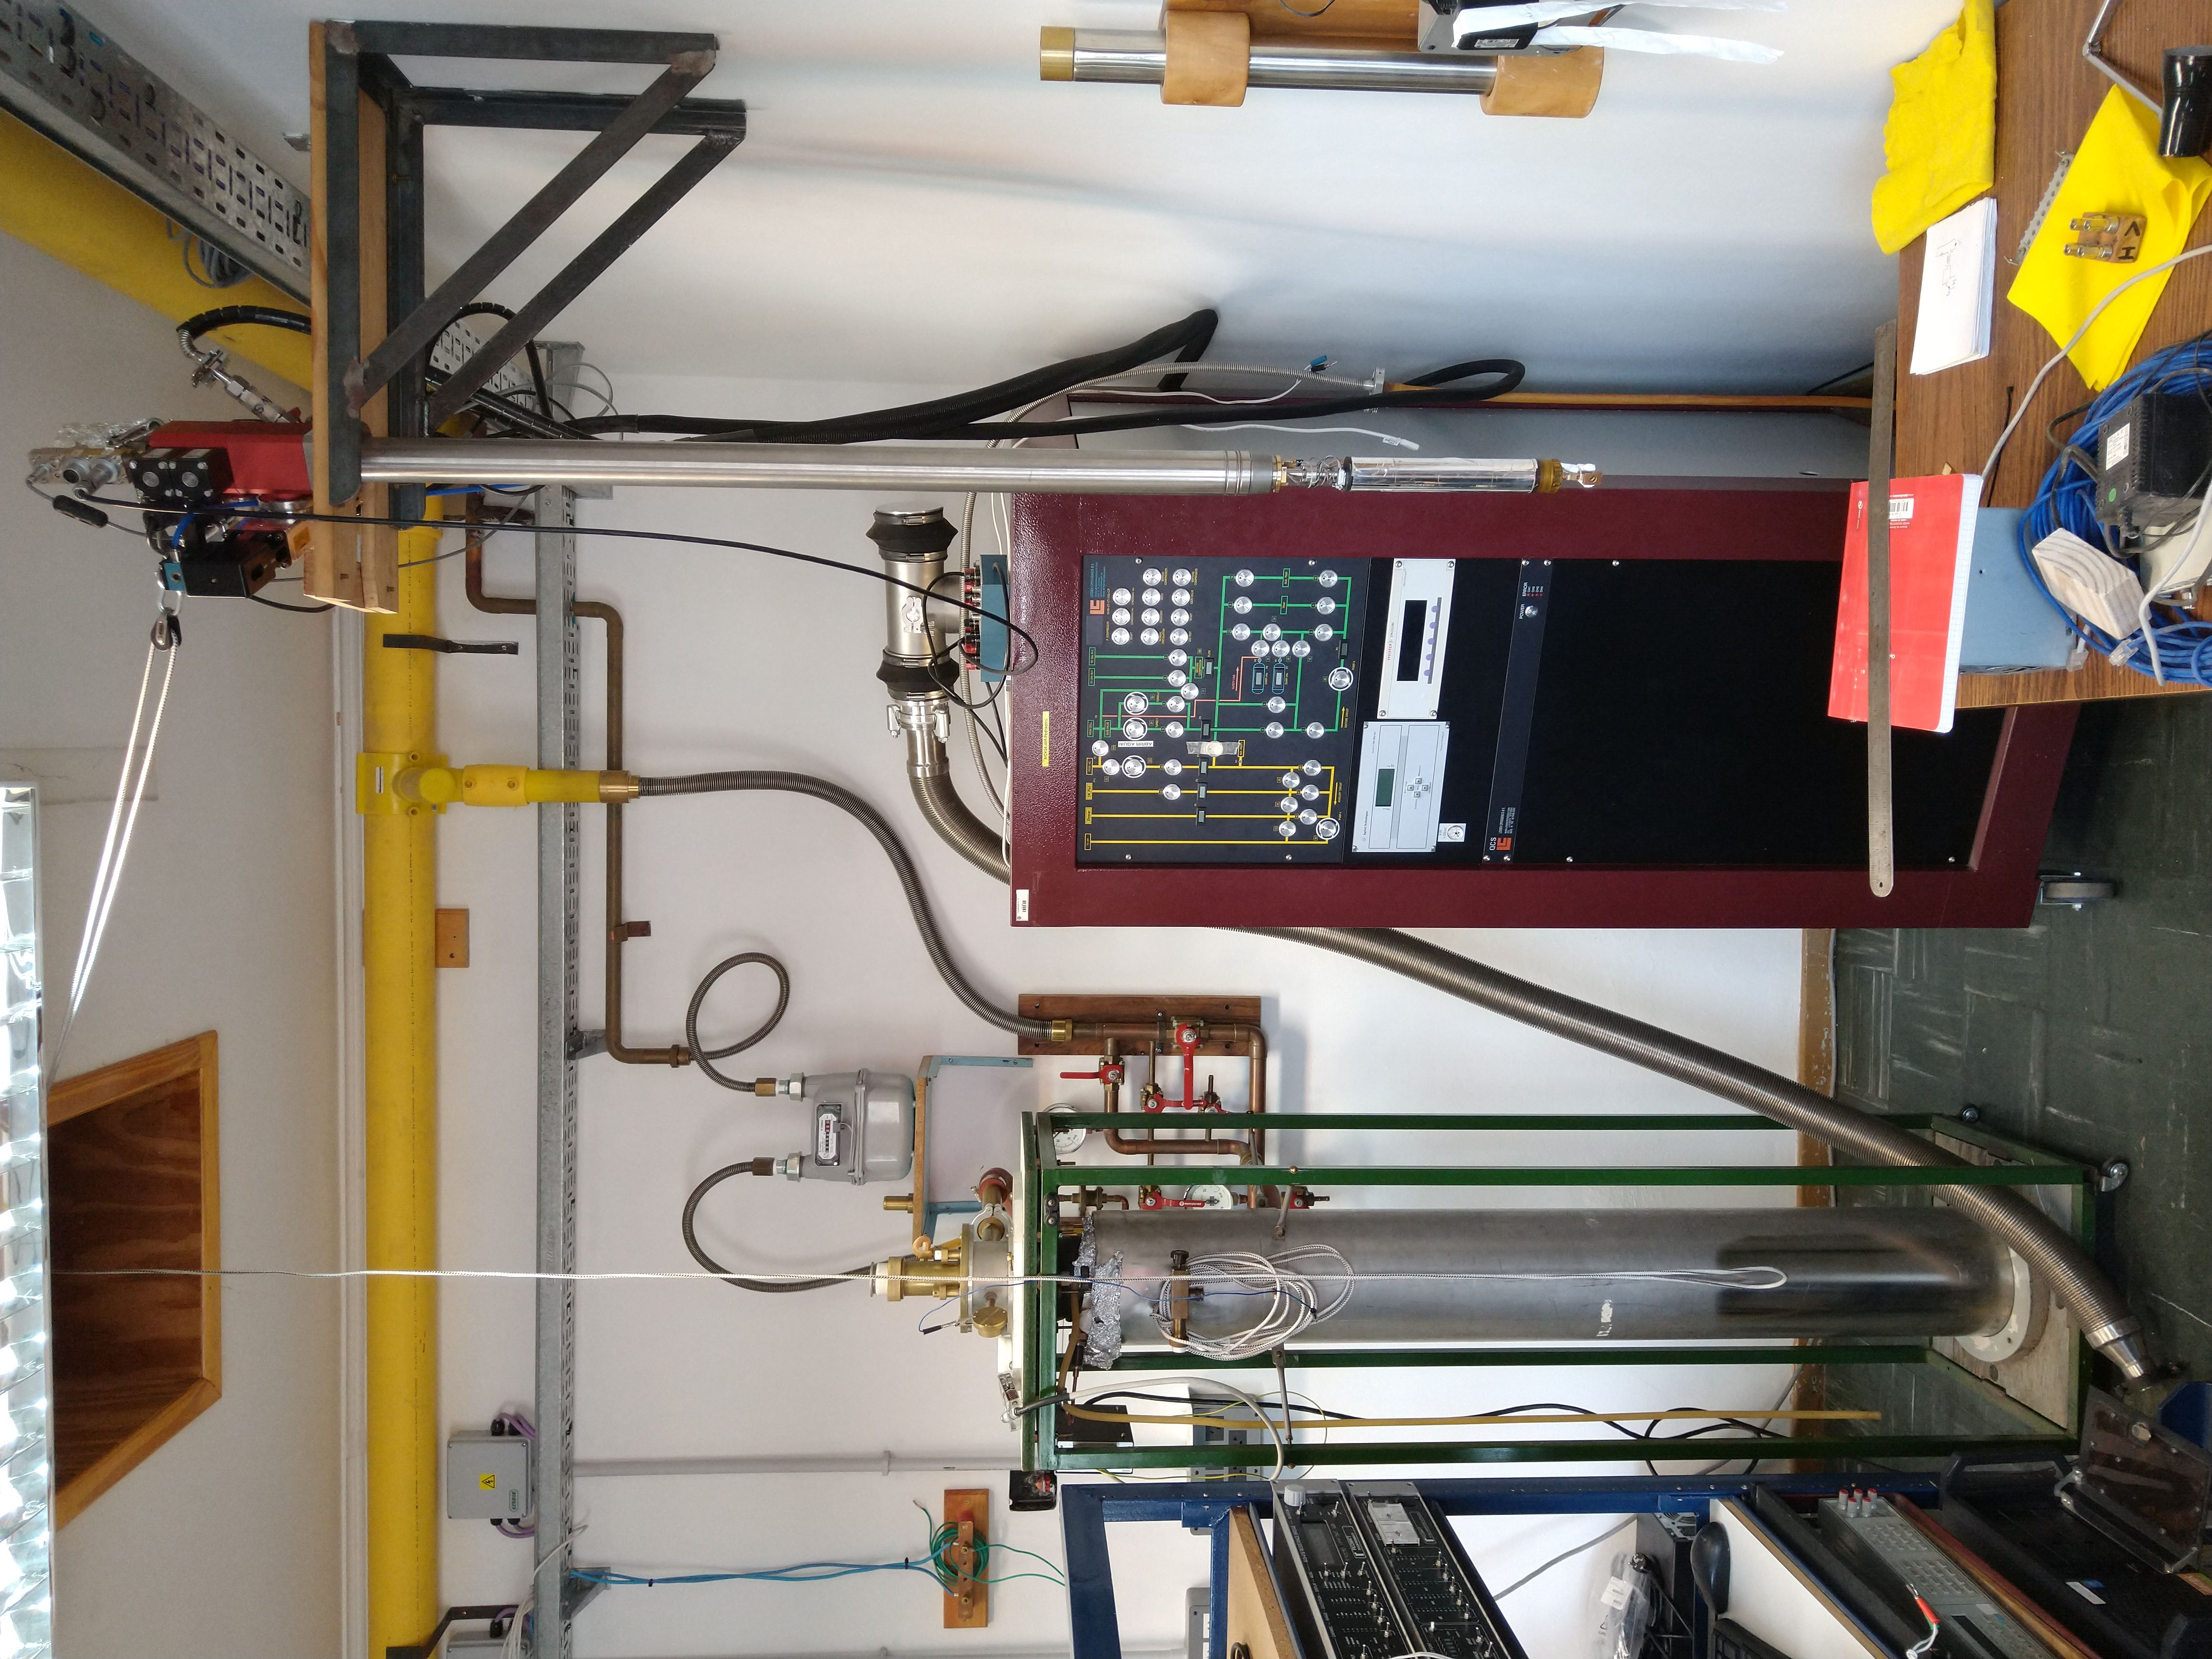
\includegraphics[angle=-90,width=0.6\textwidth]{IMG_20190523_105117465}
								\end{column}
				\end{columns}


				%				Aim for five to ten slides for a 25~minute presentation.
				%
				%				Certainly no more than 15.
				%
				%				Use a note form for the content of each slide.
				%
				%				\begin{theorem}
				%								Mathematics works within the Beamer class, $\exp(i\pi)+1=0$\,, including theorems.
				%				\end{theorem}
				%
				%				Click: \url{http://www.maths.adelaide.edu.au} 
\end{frame}

\begin{frame}{Equipos BT}
				\begin{columns}
								\begin{column}{0.45\textwidth}
												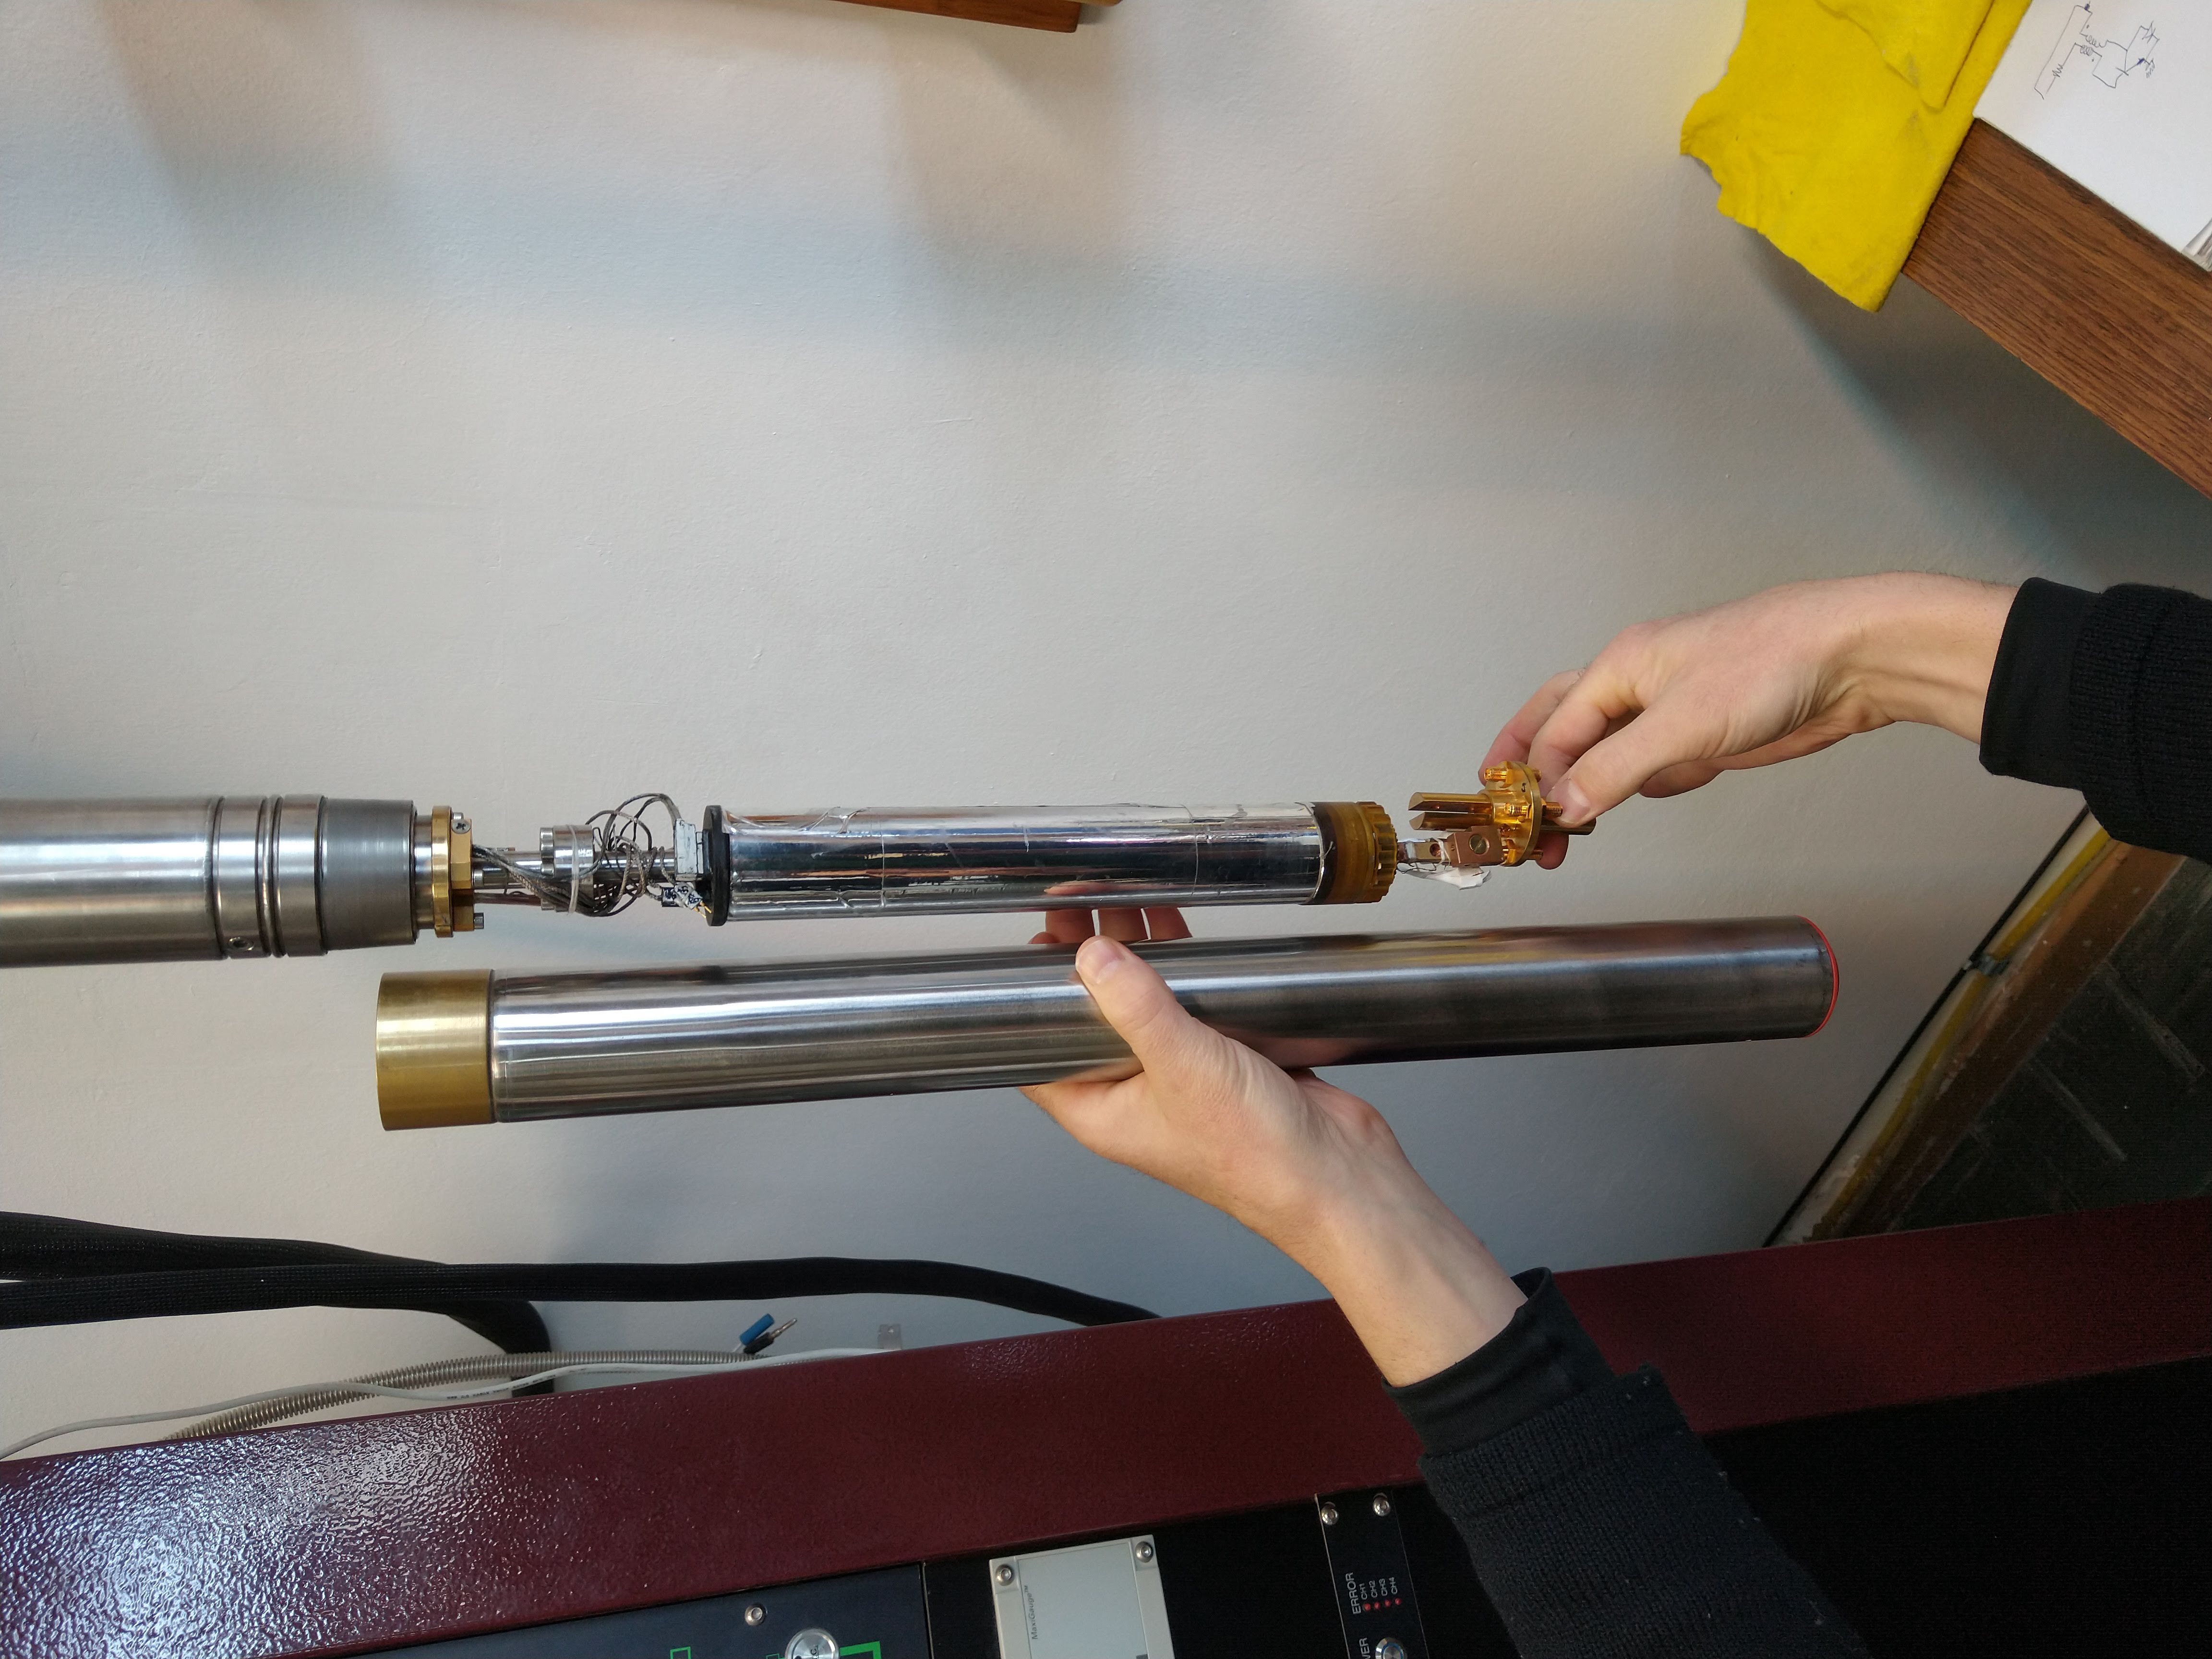
\includegraphics[angle=-90,width=0.62\textwidth]{IMG_20190523_111114131} \\ 
												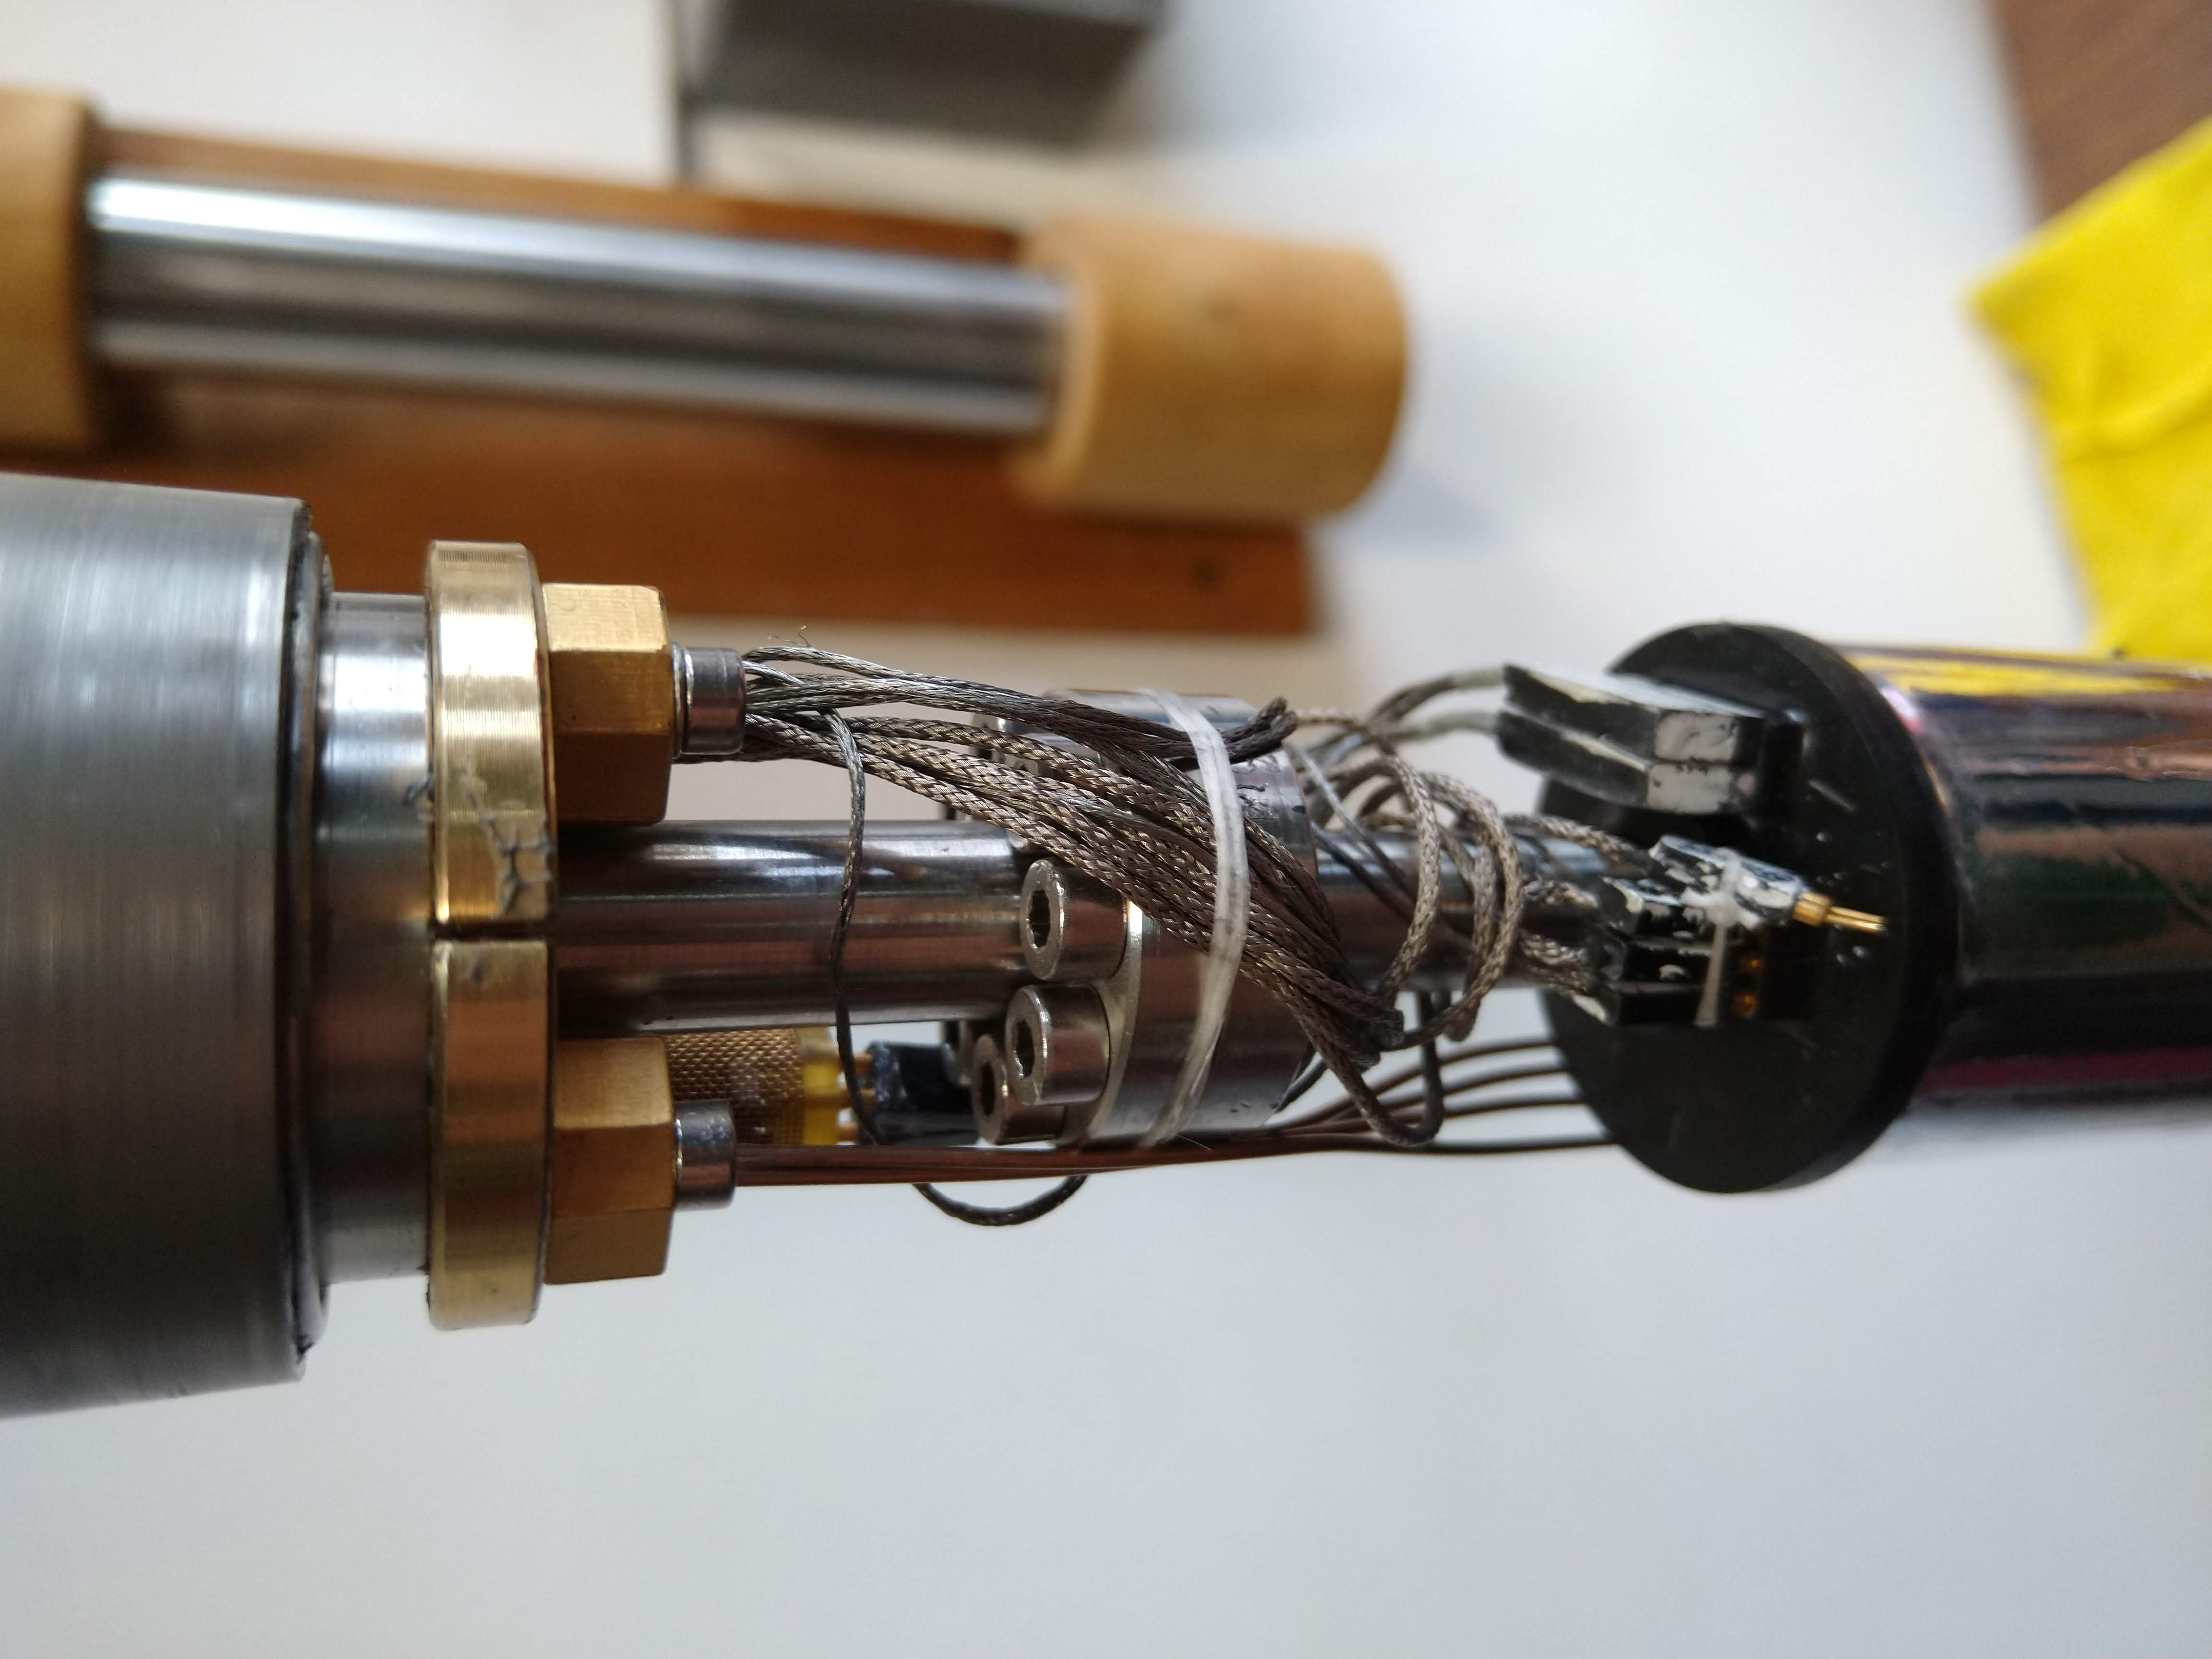
\includegraphics[angle=-90,width=0.6\textwidth]{IMG_20190523_105054061}
								\end{column}
								\begin{column}{0.45\textwidth}
												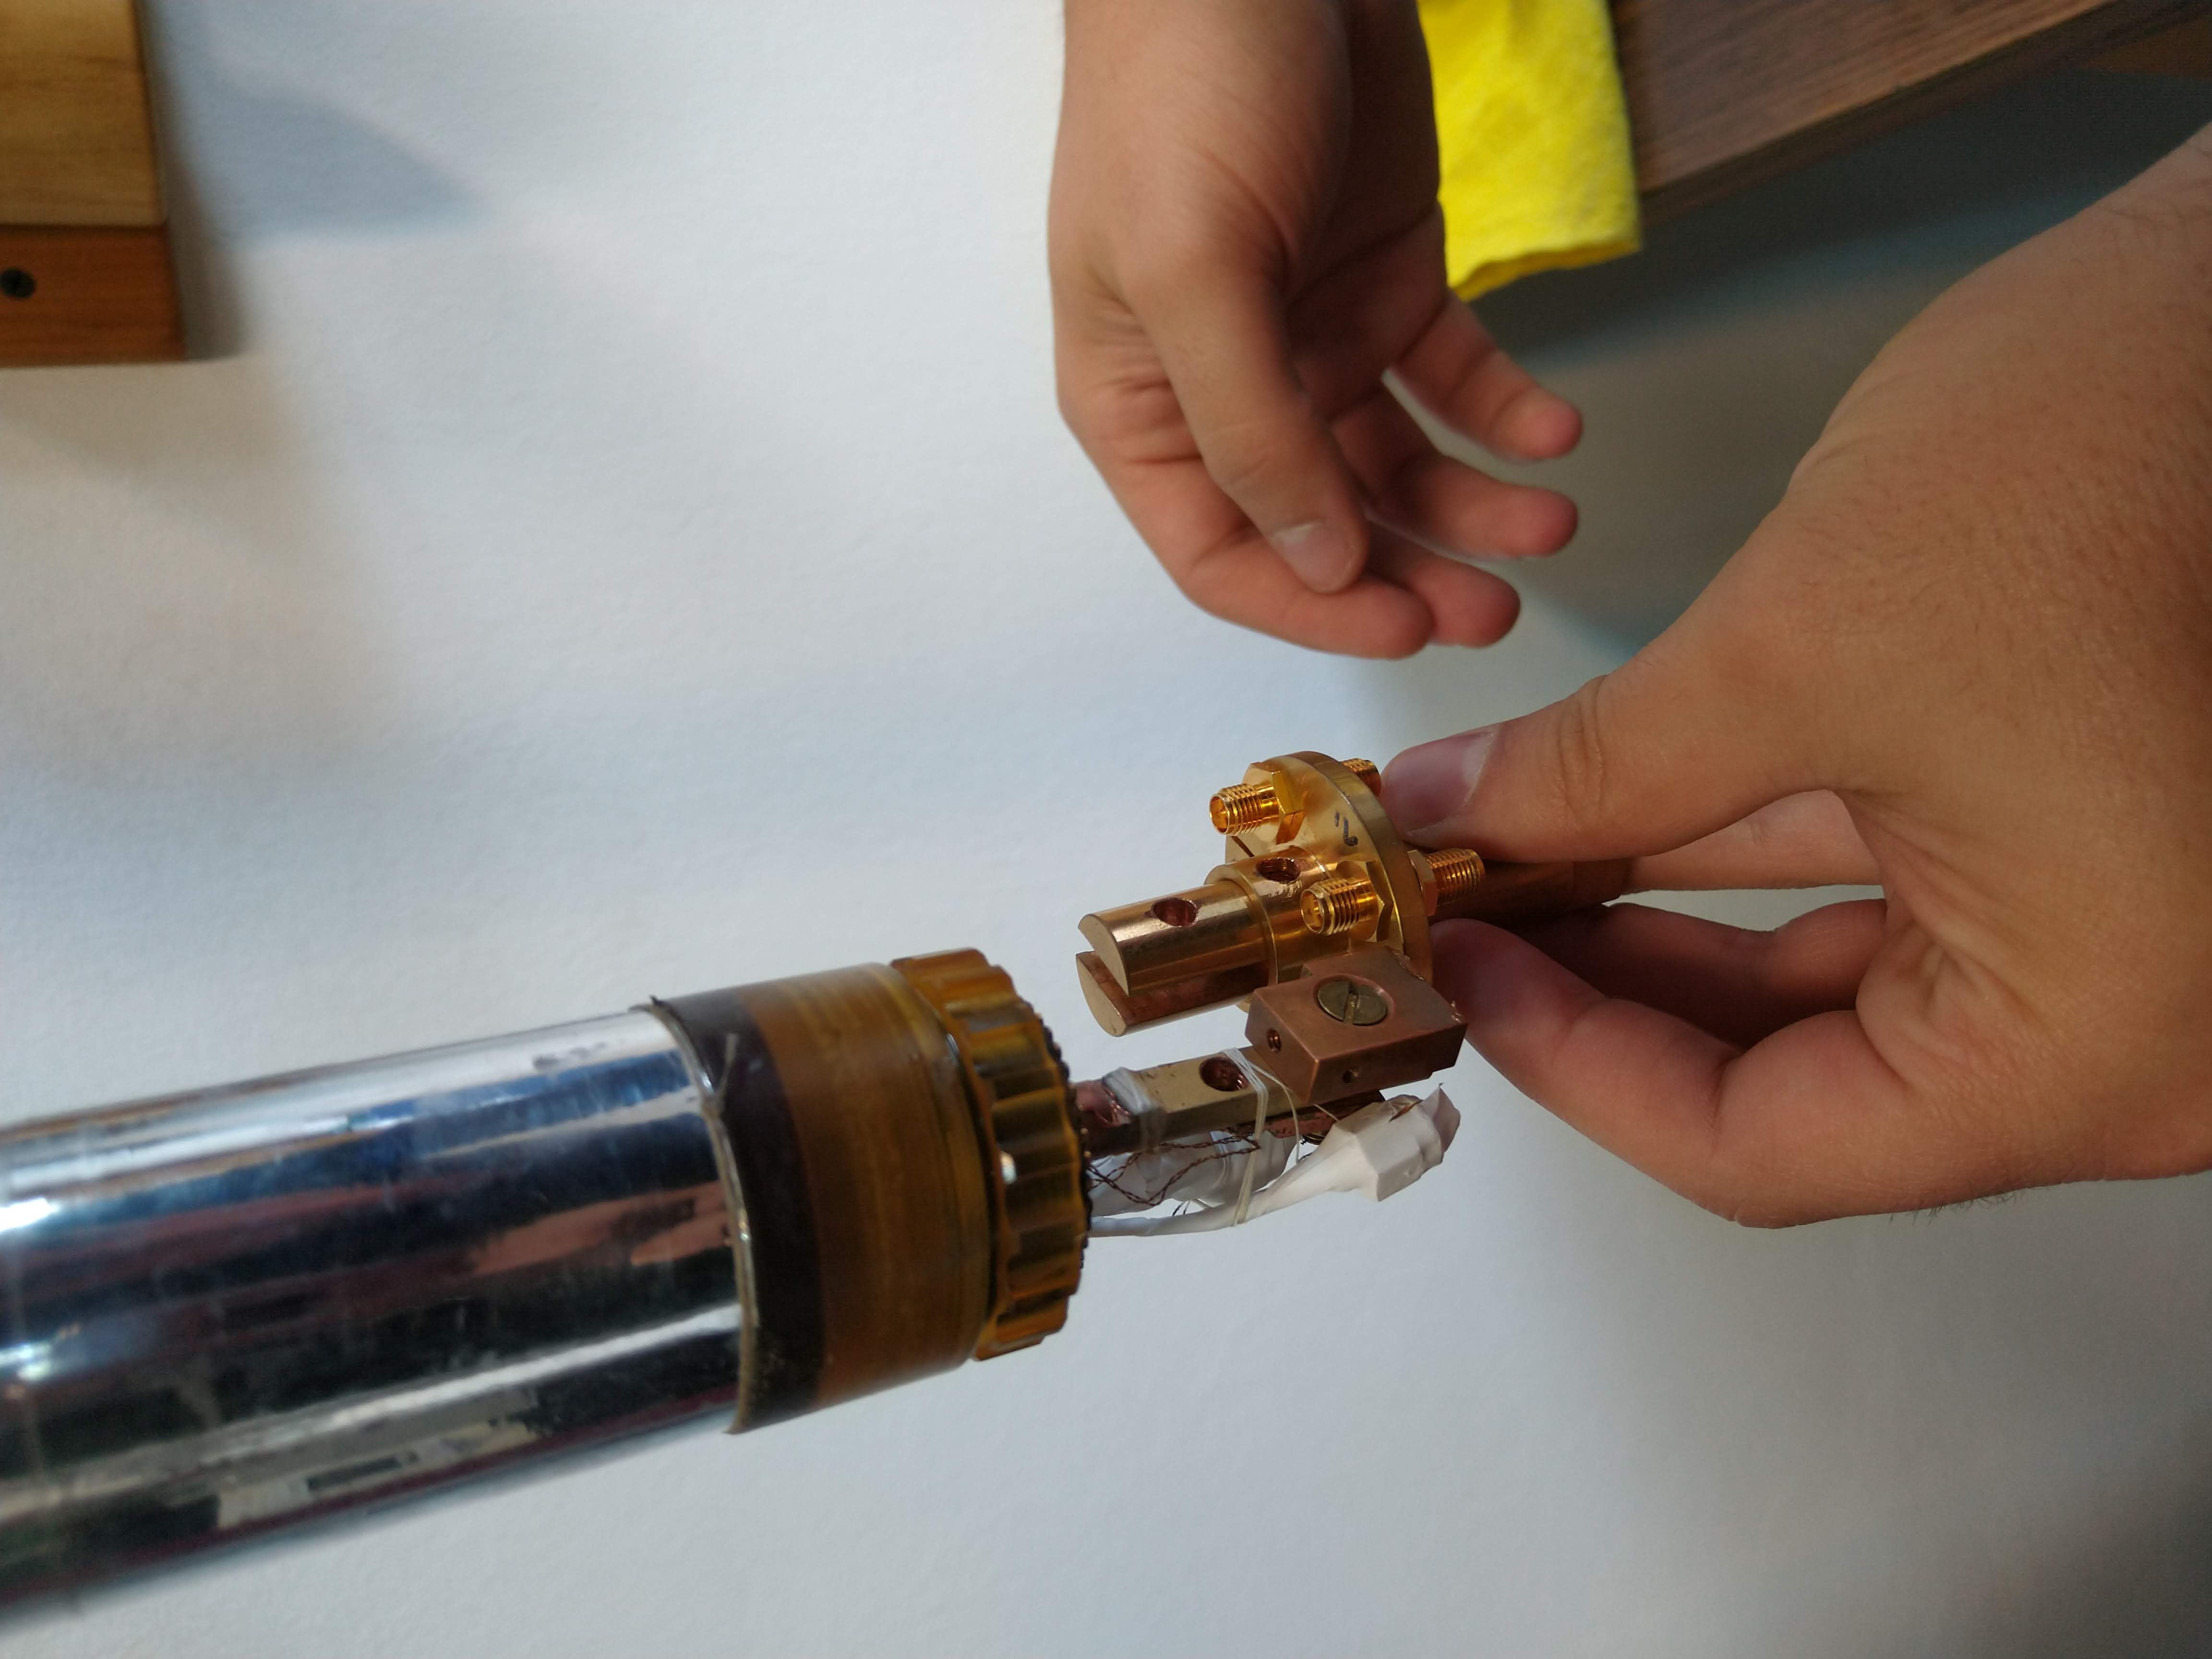
\includegraphics[angle=-90,width=0.42\textwidth]{IMG_20190523_105647049} \\ 
												\hspace{2mm}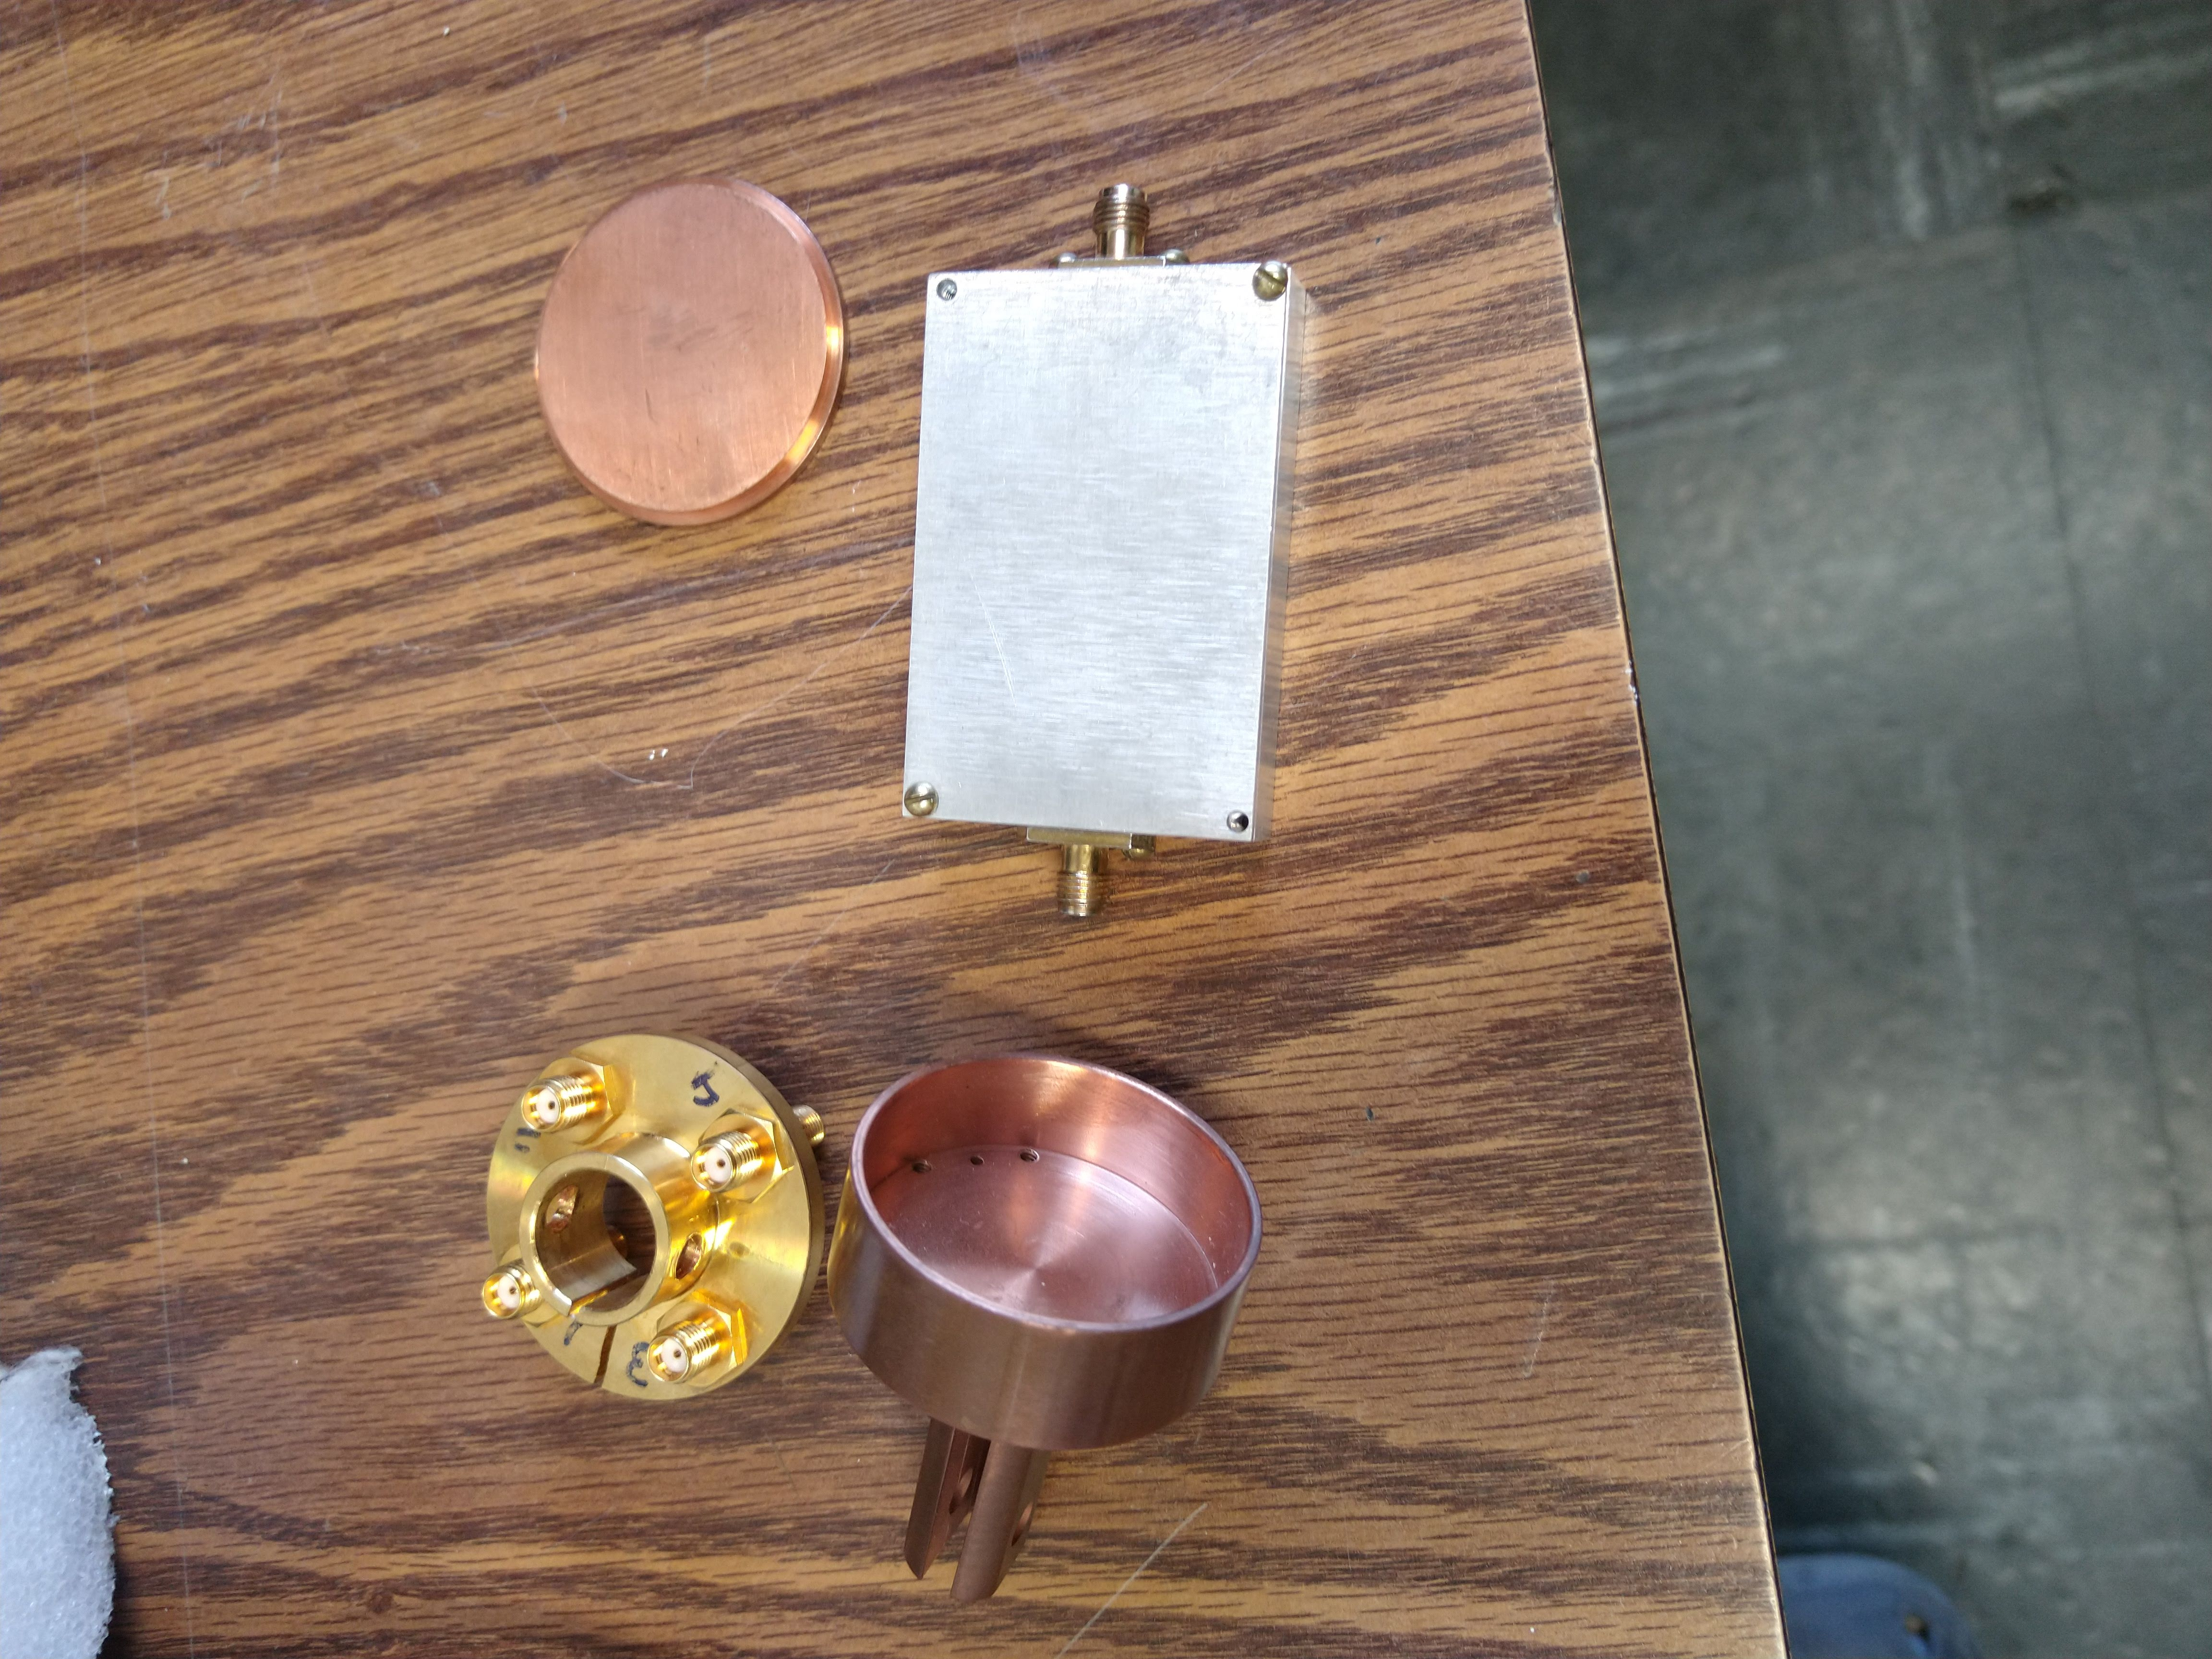
\includegraphics[angle=-90,width=0.42\textwidth]{IMG_20190523_112752228} \\
												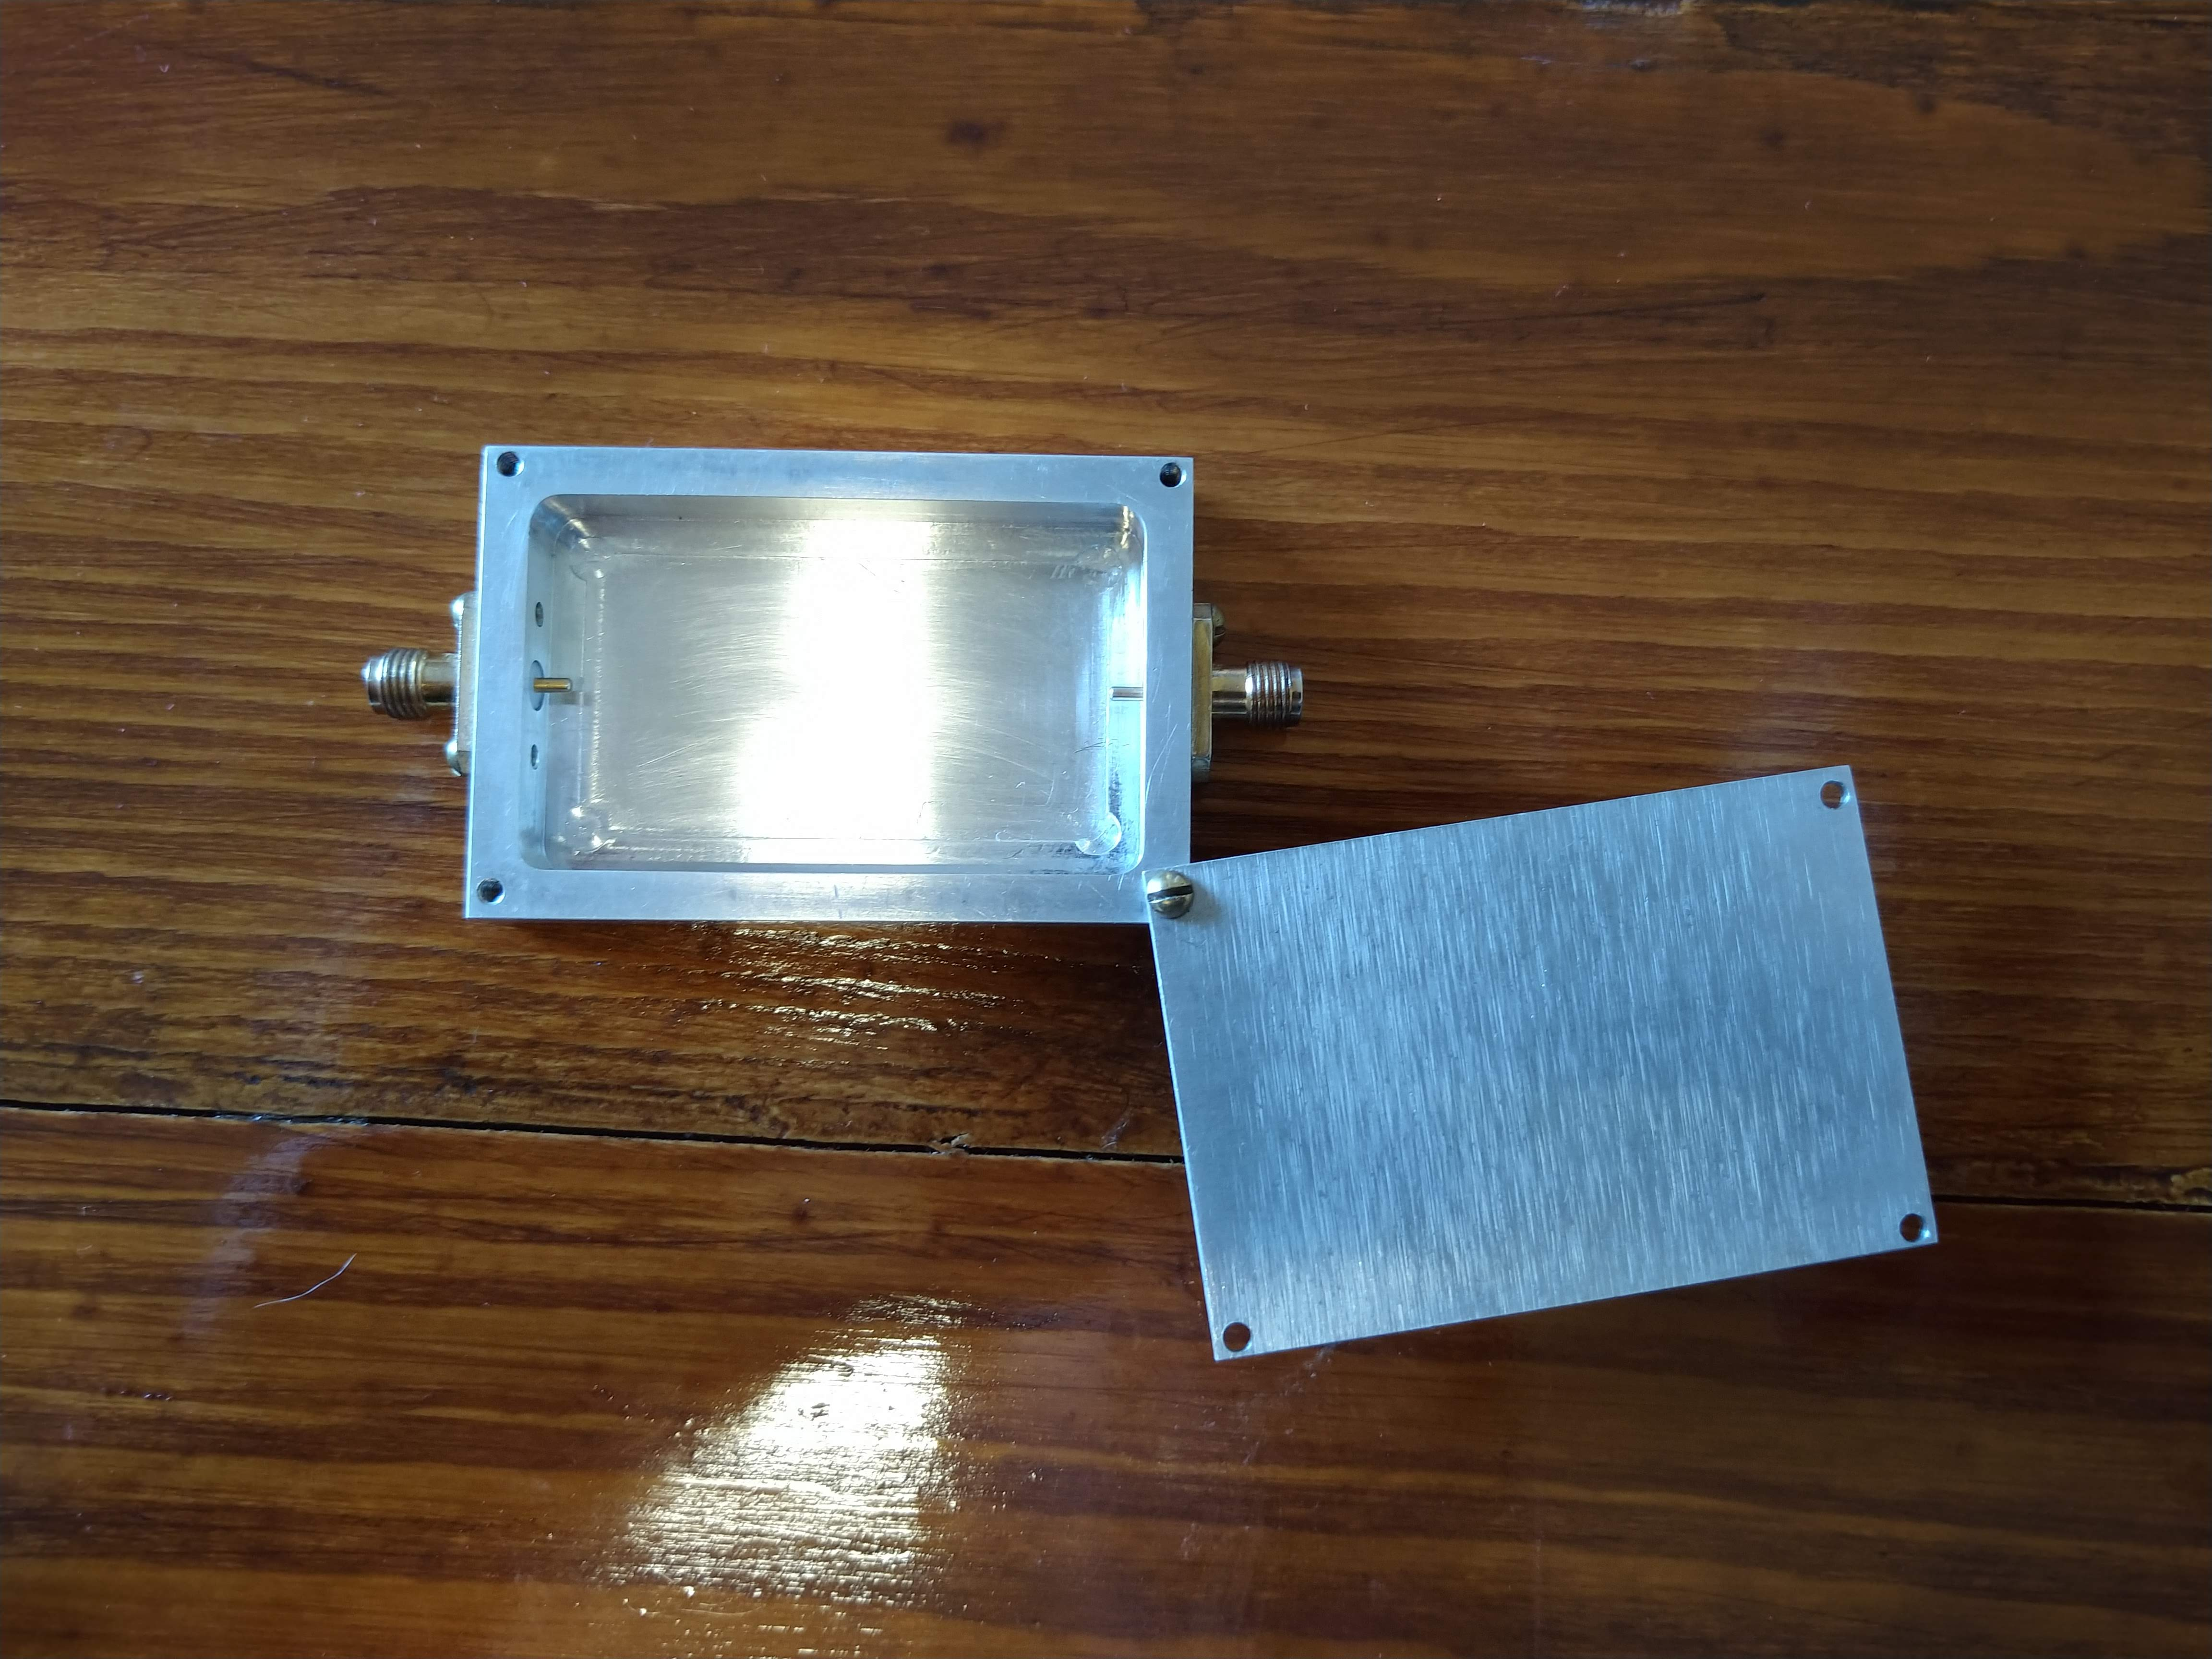
\includegraphics[angle=-90,width=0.42\textwidth]{IMG_20190523_104038976}
								\end{column}
				\end{columns}
				%				Aim for five to ten slides for a 25~minute presentation.
				%
				%				Certainly no more than 15.
				%
				%				Use a note form for the content of each slide.
				%
				%				\begin{theorem}
				%								Mathematics works within the Beamer class, $\exp(i\pi)+1=0$\,, including theorems.
				%				\end{theorem}
				%
				%				Click: \url{http://www.maths.adelaide.edu.au} 
\end{frame}

				\begin{frame}{Amplificador criog\'enico de bajo ruido}
								\framesubtitle{LNF-LNC03\_14A}
								\begin{columns}
												\begin{column}{0.40\textwidth}
																\hspace{10mm}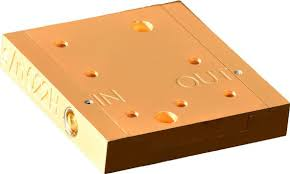
\includegraphics[width=0.95\textwidth]{lnf-lnc03_14sa}
												\end{column}
												\begin{column}{0.60\textwidth}
																\begin{itemize}
																				\item Ancho de Banda RF: 0.3-14 GHz
																				\item Ruido: 4.1 K (típico)
																				\item Ganancia: 42 dB
																				\item Potencia DC: Vc= 0.7 V @ 14 mA
																				\item Conectores RF: G3PO Macho
																				\item Conector DC: Nano Strip 5 pines hembra
																\end{itemize}
												\end{column}
								\end{columns}
				\end{frame}



				%------------------------------------------------------------------------------
\section{Mediciones}
\begin{frame}{Barrido en potencia}
				\centering
												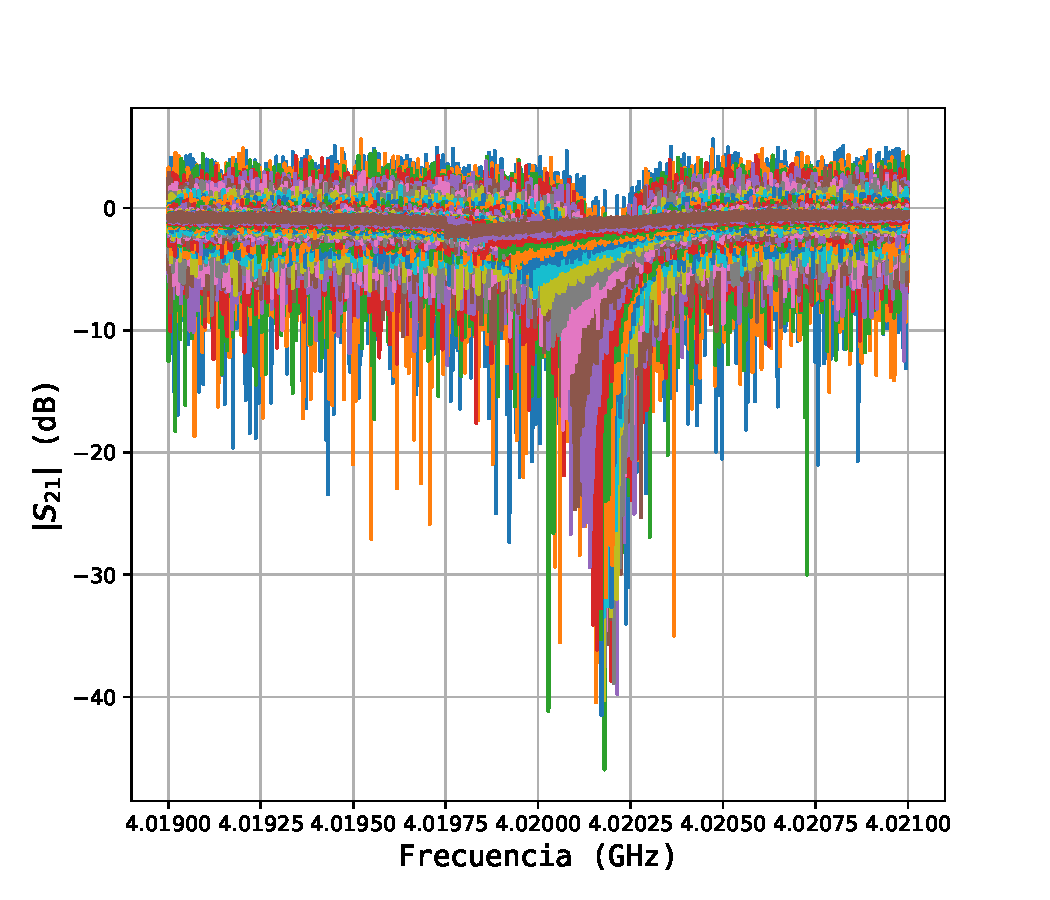
\includegraphics[width=0.62\textwidth]{resonador0_asc_sin_filtro}
												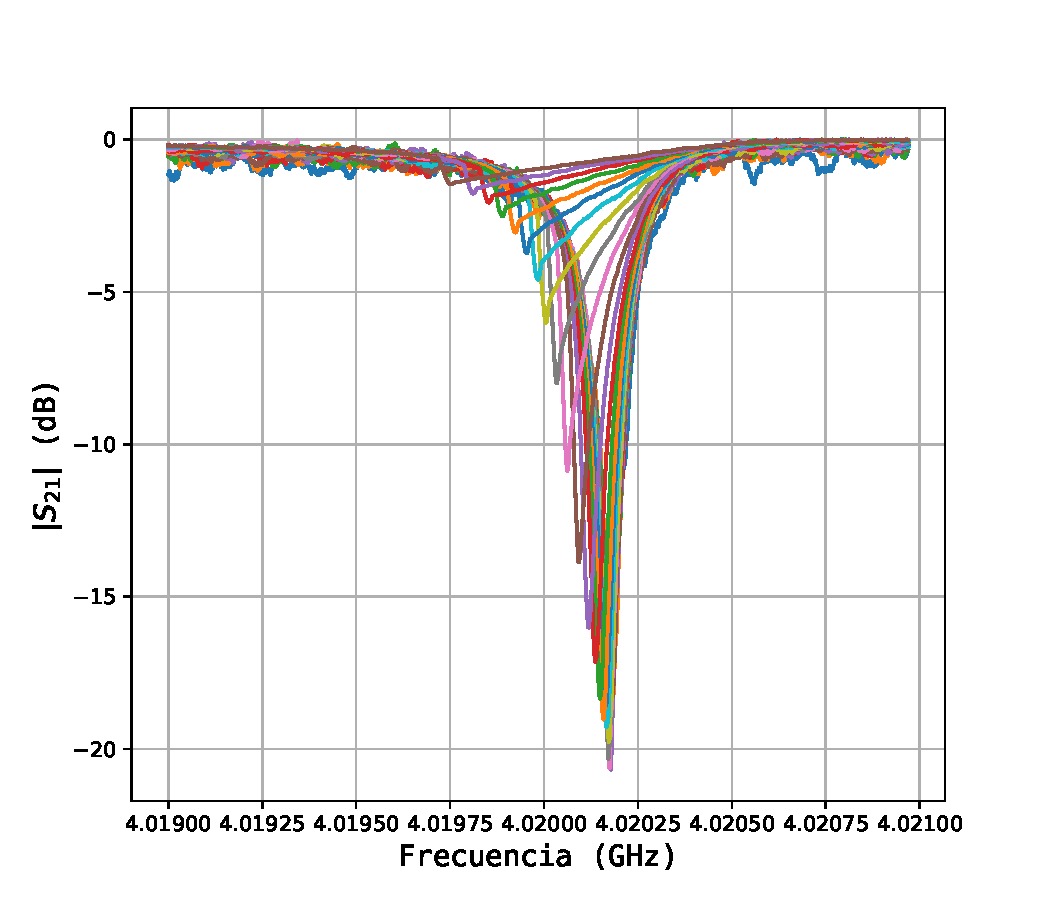
\includegraphics[width=0.62\textwidth]{resonador0_asc_filtro}
\end{frame}
\begin{frame}{Barrido en potencia}
				\centering
												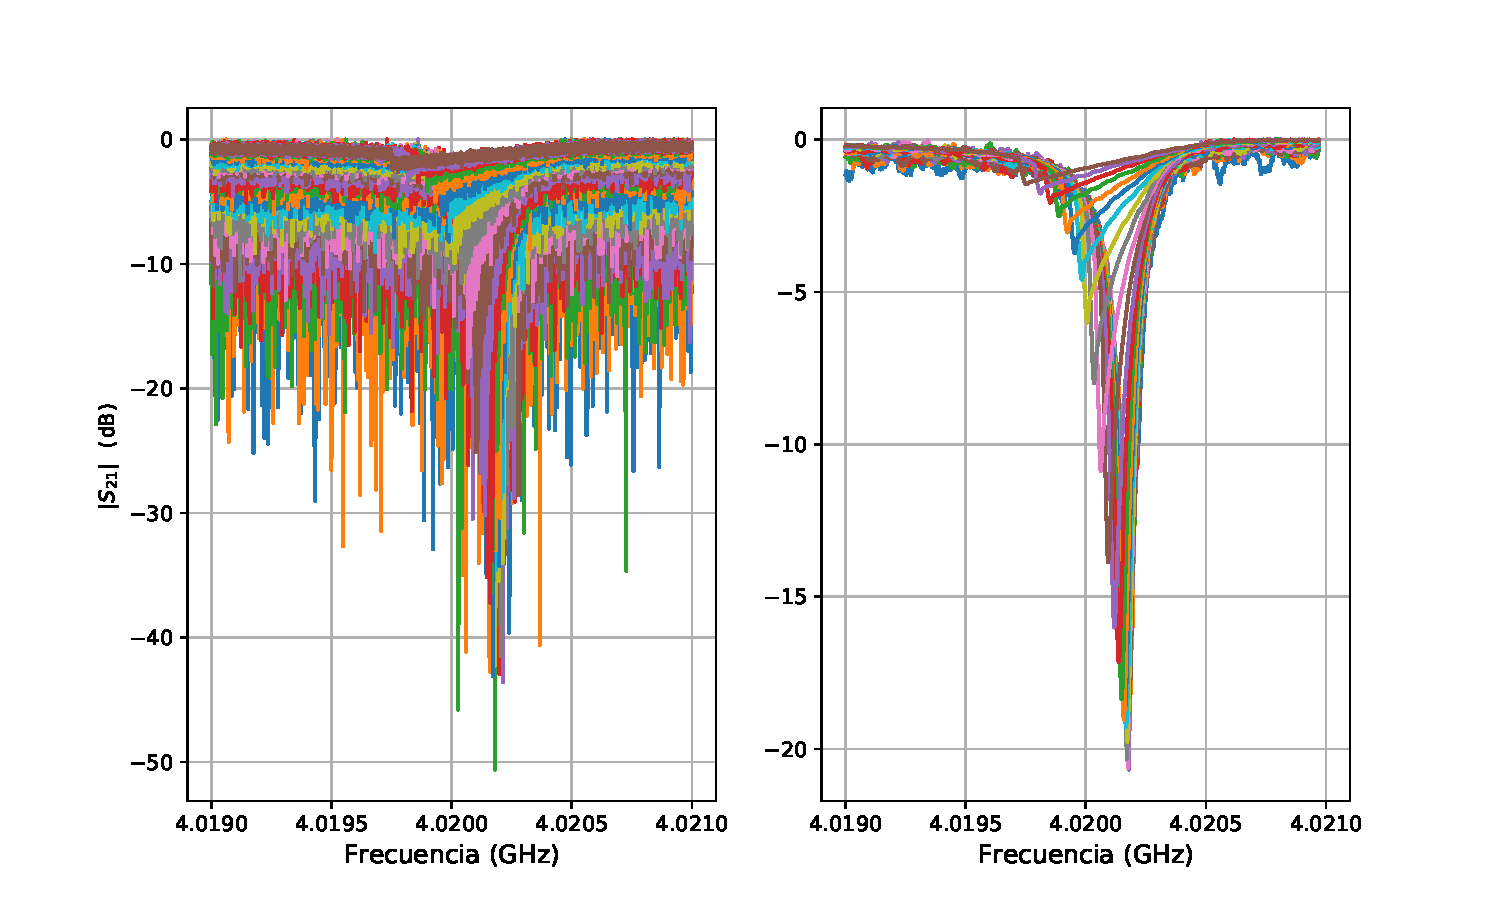
\includegraphics[width=0.62\textwidth]{res0_full_potencias}
\end{frame}
\begin{frame}{Barrido en potencia}
				\centering
												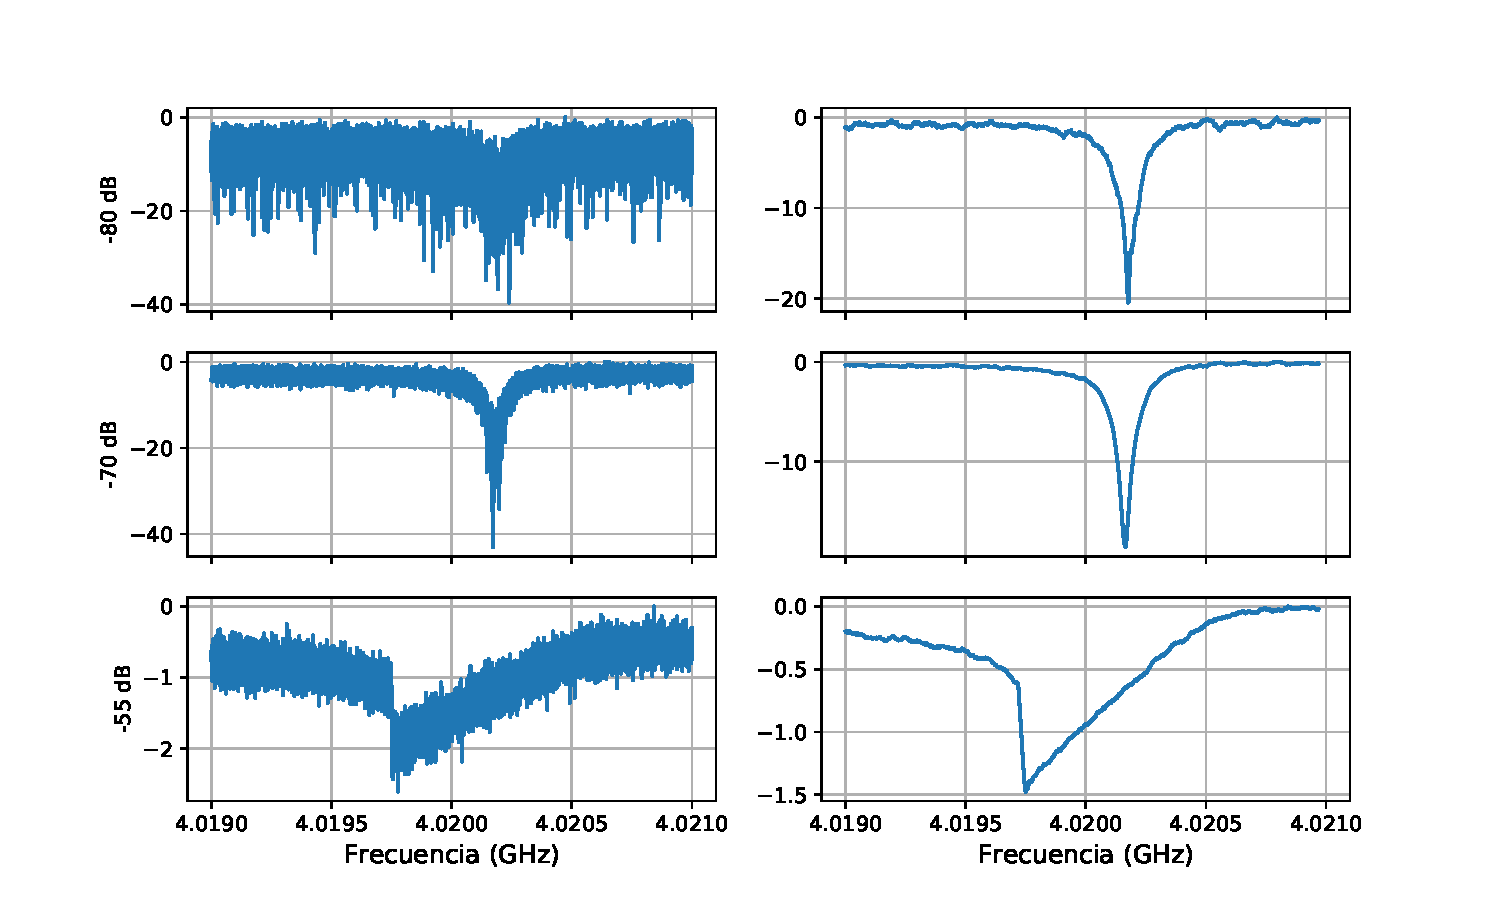
\includegraphics[width=0.82\textwidth]{res0_3_potencias}

\end{frame}
\begin{frame}{Barrido en potencia}
				\centering
												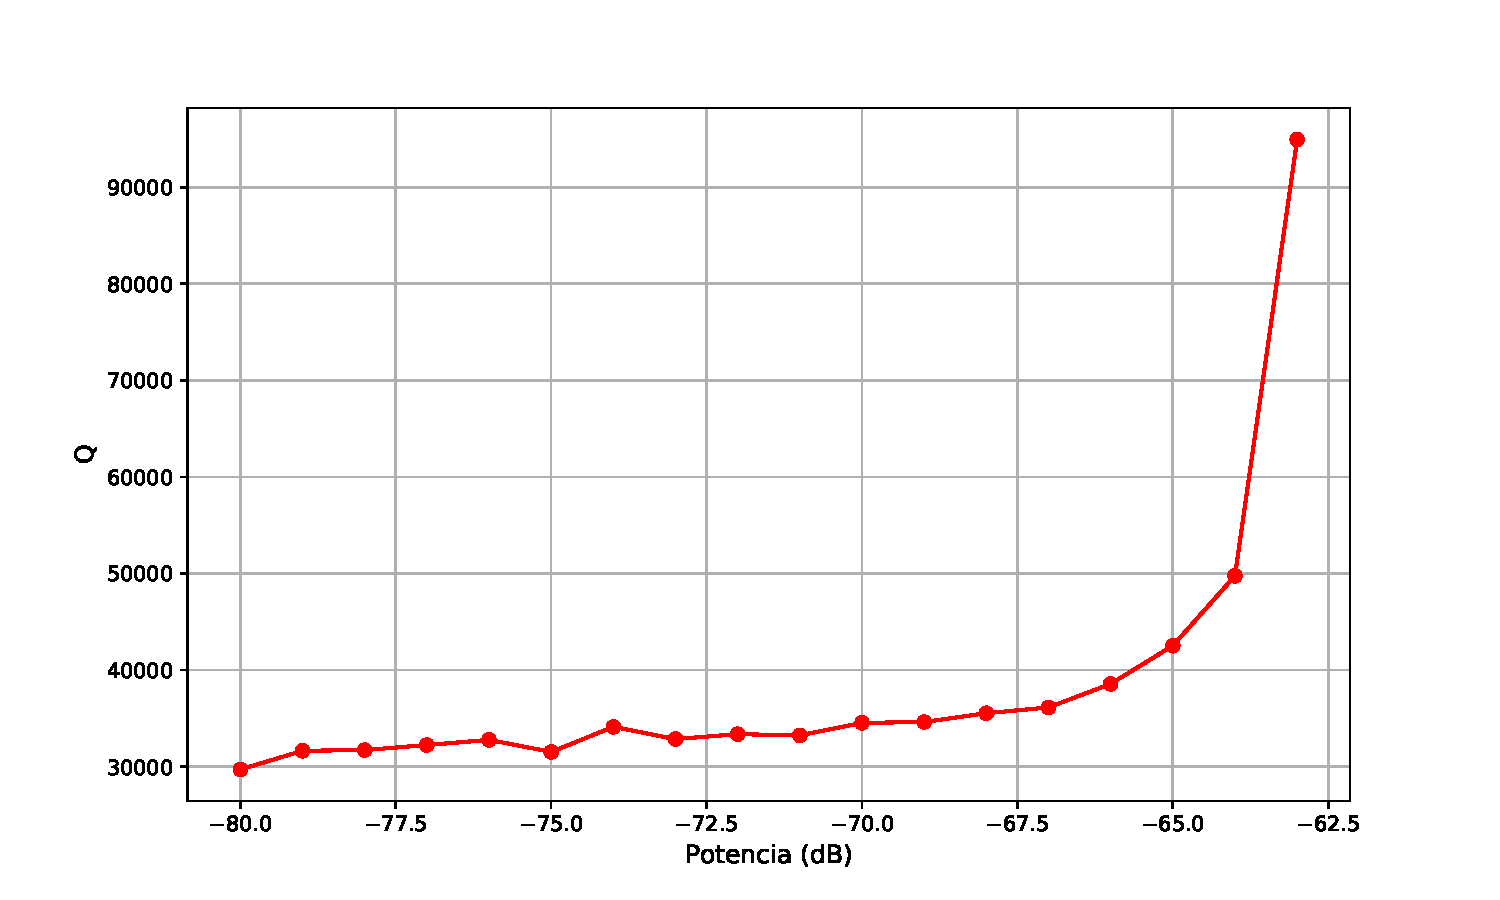
\includegraphics[width=0.82\textwidth]{res0_Q_vs_P}

\end{frame}


\section{Perspectivas de trabajo}
\begin{frame}{Perspectivas de trabajo}
				\begin{itemize}
								\item Dise\~no de resonador en Sonnet
								\item Primeras mediciones a $T_{amb}$ y $T \sim 100\,mK$
								\item Definici\'on de requerimientos para crio (cables,
												conectores, espacios, etc.)
								\item Primeras pruebas con RxChannelizer con ITeDA (pruebas de
												front-end, mezcladores, filtros, DC-block, etc.)
				\end{itemize}
\end{frame}
\section{MKIDs}
\begin{frame}{MKIDs}
				\begin{columns}
								\begin{column}{0.49\textwidth}
												\centering
												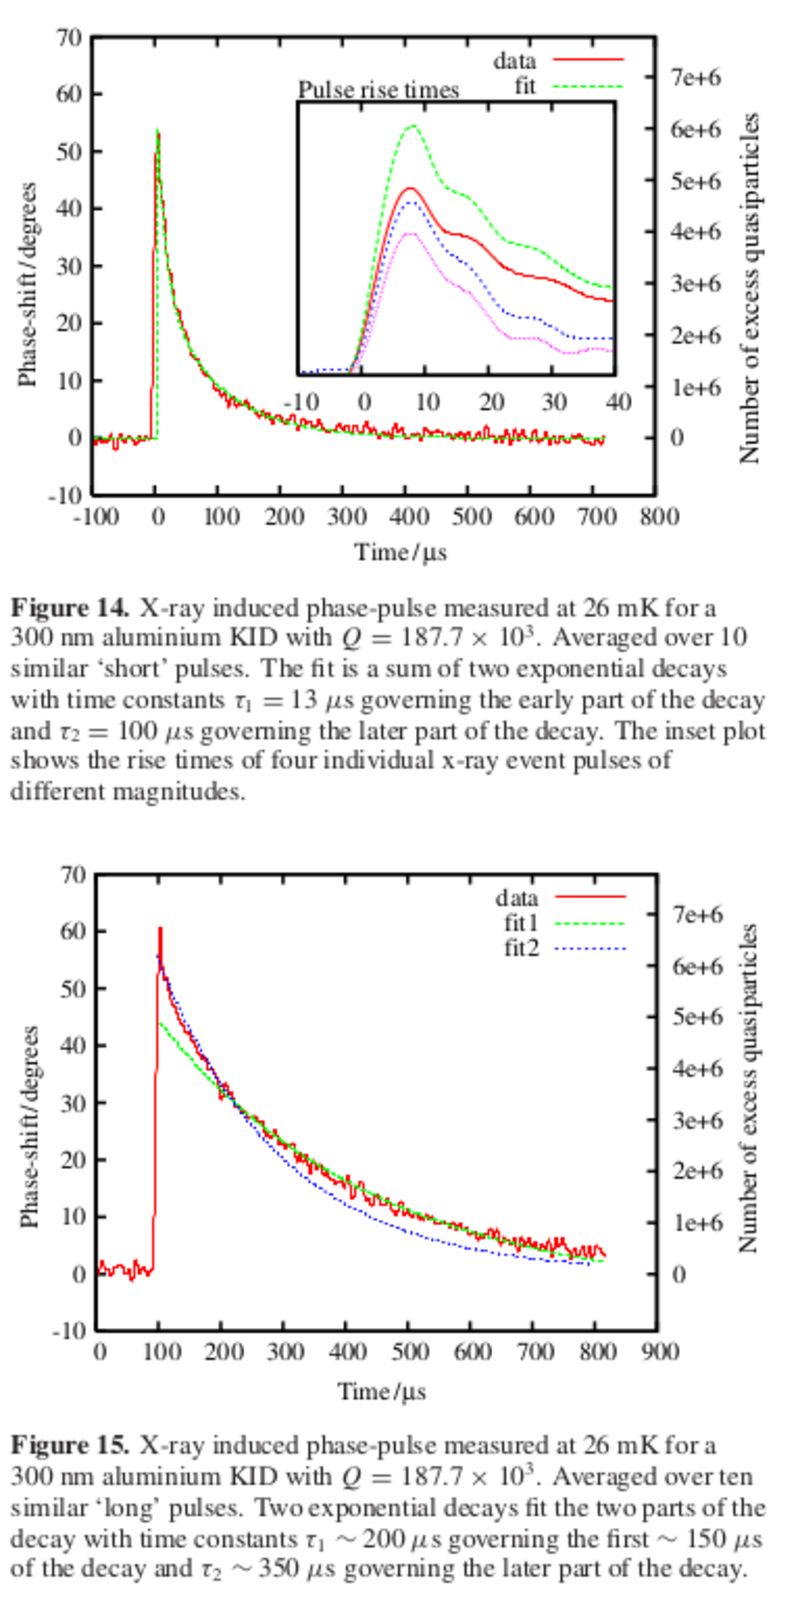
\includegraphics[width=0.62\textwidth]{pulso_respuesta_mkid}
								\end{column}
								\begin{column}{0.49\textwidth}
												\footnotesize{The KID detection mechanism $\to$ a
												temporal change in the surface kinetic inductance
												of a superconductor when a photon of energy $h\nu \geq
												2 \Delta(T)$ is absorbed, where $\Delta(T)$ is the
												superconducting gap parameter. 
												\pause

												High energy photons break
												Cooper pairs. These recombine in a characteristic time,
												of the order $10-500\,\mu\text{s}$,
												{\color{red}producing pulse-like changes in the surface
												impedance}. 
												\pause

												As the impedance of a superconductor is
												mostly inductive, especially for $T << T_c$, the
												superconductor can be engineered as the inductive
												element in a RLC-like resonant circuit. 
												\pause

												{\color{blue}The
												quality factor of the resonant circuit determines both the
												\alert{sensitivity} and \alert{speed} of the device}.}
								\end{column}
				\end{columns}
\end{frame}

\begin{frame}{MKIDs}
				\framesubtitle{Energy resolution}
				%\begin{exampleblock}{}
				%				Works on the principle that incident photons change the surface
				%				impedance of a superconductor through the \textit{kinetic
				%				inductance effect}
				%\end{exampleblock}
												\begin{equation}
																R = \frac{1}{2.355}\sqrt{\frac{\eta h \nu}{F
																\Delta}}
												\end{equation}
				$\eta = 0.57 \to$ efficiency of creating quasiparticles, 

				$h\nu \to$ energy of the incident photon, 

				$\Delta = 1.72 k_BT_c \to$ gap energy of the superconducting absorber, 

				$F \approx 0.2 \to$ Fano factor 

				$R=150$ at 5\,eV for an operating temperature of 100\,mK. 

				An operating temperature of 15\,mK could allow a theoretical
				maximum energy resolution of $R=400$ at 5\,eV (although it is likely other
				noise sources, like two level system noise, will become more important
				as future development increases the energy resolution).

\end{frame}
\begin{frame}{MKIDs}
				%\begin{exampleblock}{}
				%				Works on the principle that incident photons change the surface
				%				impedance of a superconductor through the \textit{kinetic
				%				inductance effect}
				%\end{exampleblock}
				\scriptsize{\begin{itemize}
								\item Serve as mm/submm photon detectors
								\item Resonance  $1-10\,\text{GHz}$ 
								\item $Q \sim 10^5$
								\item $T_{op} < 300\,\text{mK}$
								\item Intrinsic energy resolution $R = \frac{E}{\Delta E} \sim
												20-150$\footnote{Rev.Sci.Instr. 83, 044702 (2012)}
								\item The resonators are designed to be separated by 2\,MHz
												within a $4-5\,\text{GHz}$ band.
								\item Off-resonance transmission $\simeq 1$
												%				\begin{equation}
												%								R = \frac{1}{2.355}\sqrt{\frac{\eta h \nu}{F
												%								\Delta}}
												%				\end{equation}
				\end{itemize}
				Each resonator will have a $BW \sim 200\,\text{kHz}$ (\alert{based on the
				quality factor we need}),

				2\,MHz separation between the resonators is required (resonator position
				will move around based on different loading. If we pack them too close
				to each other, their relative position might change during observation
				or from different fridge cook down cycle). 

				So we want to have ADC to have BW at least 400\,MHz, and has SNR greater
				than 59\,dB. 

				If we just consider quantization noise, theoretically, 59\,dB SNR will
				require ADC to have at least 10 bits
				}
				%				, but in real world, we can only find 10 bits ADC
				%that has SNR greater than 59. Instead, the best we can find
				%on the market is 12 bits ADC which has SNR 64 dB and
				%up to 550 msps sampling rate. Actually once we confirmed
				%to use this ADC chips, we have also expanded the seperation
				%between resonator to 2.5 MHz.

				\tiny{\textbf{arXiv:1310.5891v2 (2013)}}
\end{frame}

\section{Readout design and development}
\begin{frame}{Readout design and development}

				%	{\color[rgb]{0.8,.4,.5} ``The readout electronics have the general task
				%	of performing multiple real-time complex microwave transmission
				%	measurements, in order to monitor the instantaneous resonance frequency
				%	and dissipation of the superconducting microresonators that serve as
				%	mm/submm photon detectors''.}

				\begin{itemize}
								\item Noise will be \alert{dominated by cryogenic amplifier (CA)}, which has noise
												temperature around 2 to 5\,K. 
								\item Besides the CA, ADC chip will be \alert{the next limiting factor for the
												noise performance of the readout}. 

								\item	Based on the physical frequency spacing of all the resonators, \alert{the
												sampling rate are chosen to match the resonator bandwidth}. 

								\item	Sampling rate of proposed readout system must be
												{\color[rgb]{0.2,0.9,0.3}flexible}.  
												%	Right now it is up to 550
												%MHz which is the limit of ADC chip.
				\end{itemize}

				\tiny{\emph{\textbf{An open-source readout for MKIDs}}, Proc. SPIE Astron.
				Telesc.  Instrum., doi:10.1117/12.856832}
\end{frame}
\begin{frame}{Readout design and development}
				\only<1>{\footnotesize{\begin{itemize}
								\item To read out an MKID, a probe tone at its resonant
												frequency is passed through it. 
								\item When a photon is absorbed by the detector, the
												phase of the tone suddenly changes. 
								\item From this change, \alert{the energy} and
												\alert{time of arrival} of the photon are determined.
								\item In the readout a complex frequency comb is
												generated by DACs and is mixed up to the range
																of resonant frequencies. 
												\item The resulting signal is sent through the MKID
																array, mixed back down to baseband, and
																digitized by ADCs. 
												\item This is then processed by \alert{firmware} on
																FPGAs, which 
																\alert{detects photon events in the phase of each
																pixel's probe tone}. 
												\item The photon data is sent to a data acquisition and
																control computer to be recorded.
				\end{itemize}}}
				\centering
				\only<2>{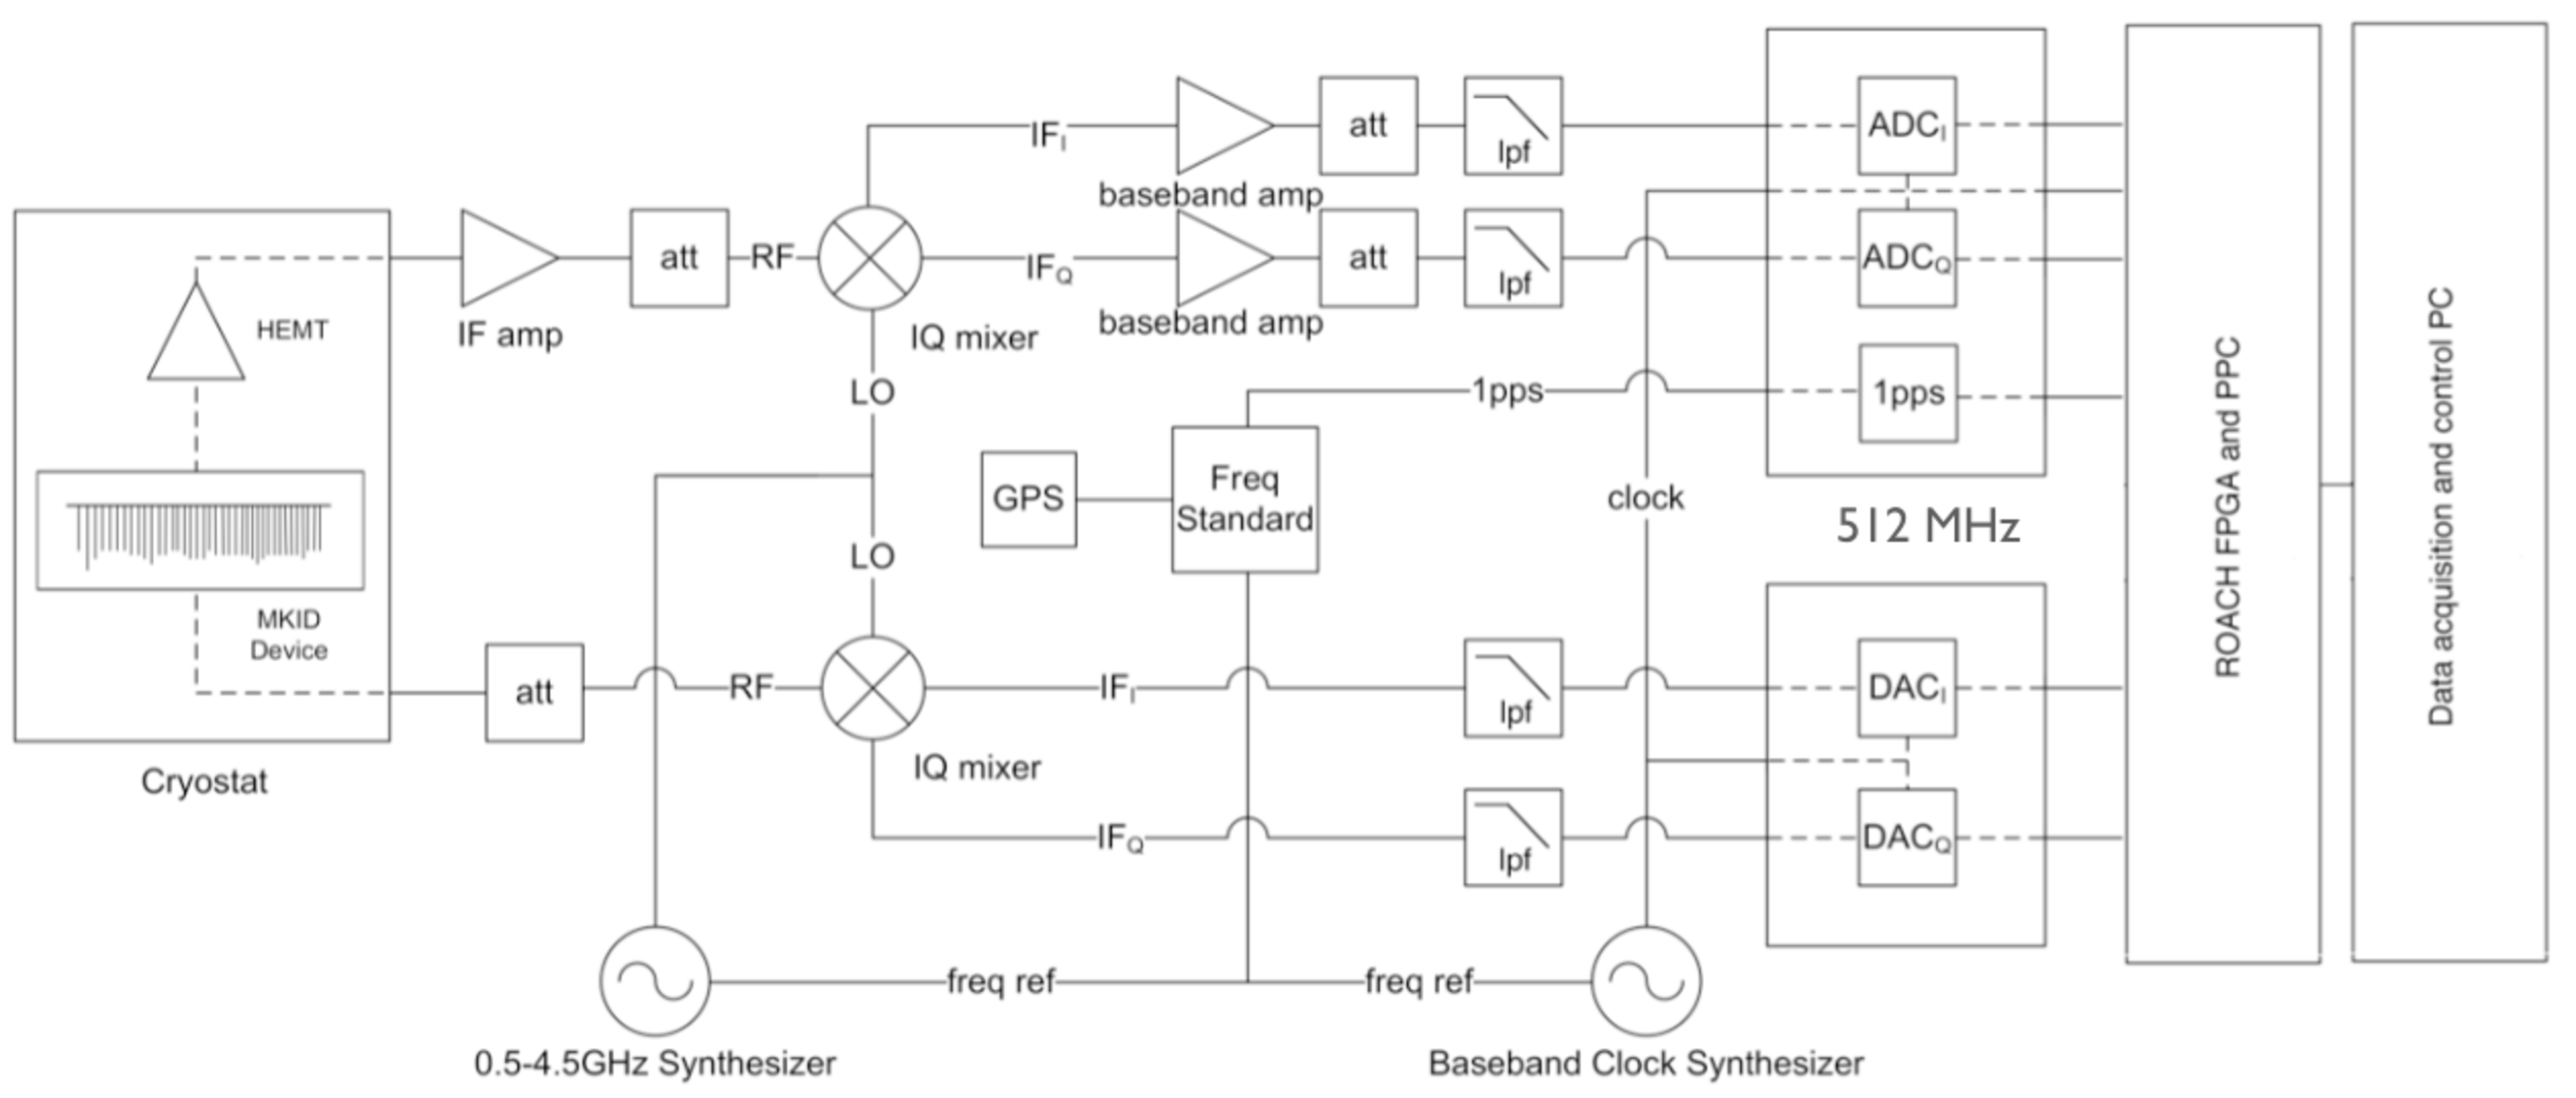
\includegraphics[width=0.8\textwidth]{arcons_readout}}
\end{frame}

\begin{frame}{Firmware}
				The firmware is written in VHDL/Verilog. 

				It controls the DAC output, and processes the ADC input. 

				It separates the digitized readout signal into frequency bins (channels)
				corresponding to each pixel. 

				The signal for each pixel is filtered and converted to phase before
				being run through \alert{pulse detection}.

				The output data rate is expected to be around 100 complex $S_{21}$
				measurements per second, per resonator\footnote{\tiny{from
				MKIDCam Readout Electronics Specifications (2008)}} $\to$ (\alert{to be
				confirmed})
\end{frame}

\begin{frame}{Pulse detection}
				\begin{columns}
								\begin{column}{0.49\textwidth}
												\scriptsize{Readout capable of recording to file one continuous
												second of phase data for one pixel at a time, \alert{sampled at
												1\,MHz}. 

												To record data from all the pixels, though, the firmware must
												reduce the data to only include data from detected photons,
												which are seen as negative peaks in the phase.}
								\end{column}
								\begin{column}{0.49\textwidth}
												\centering
												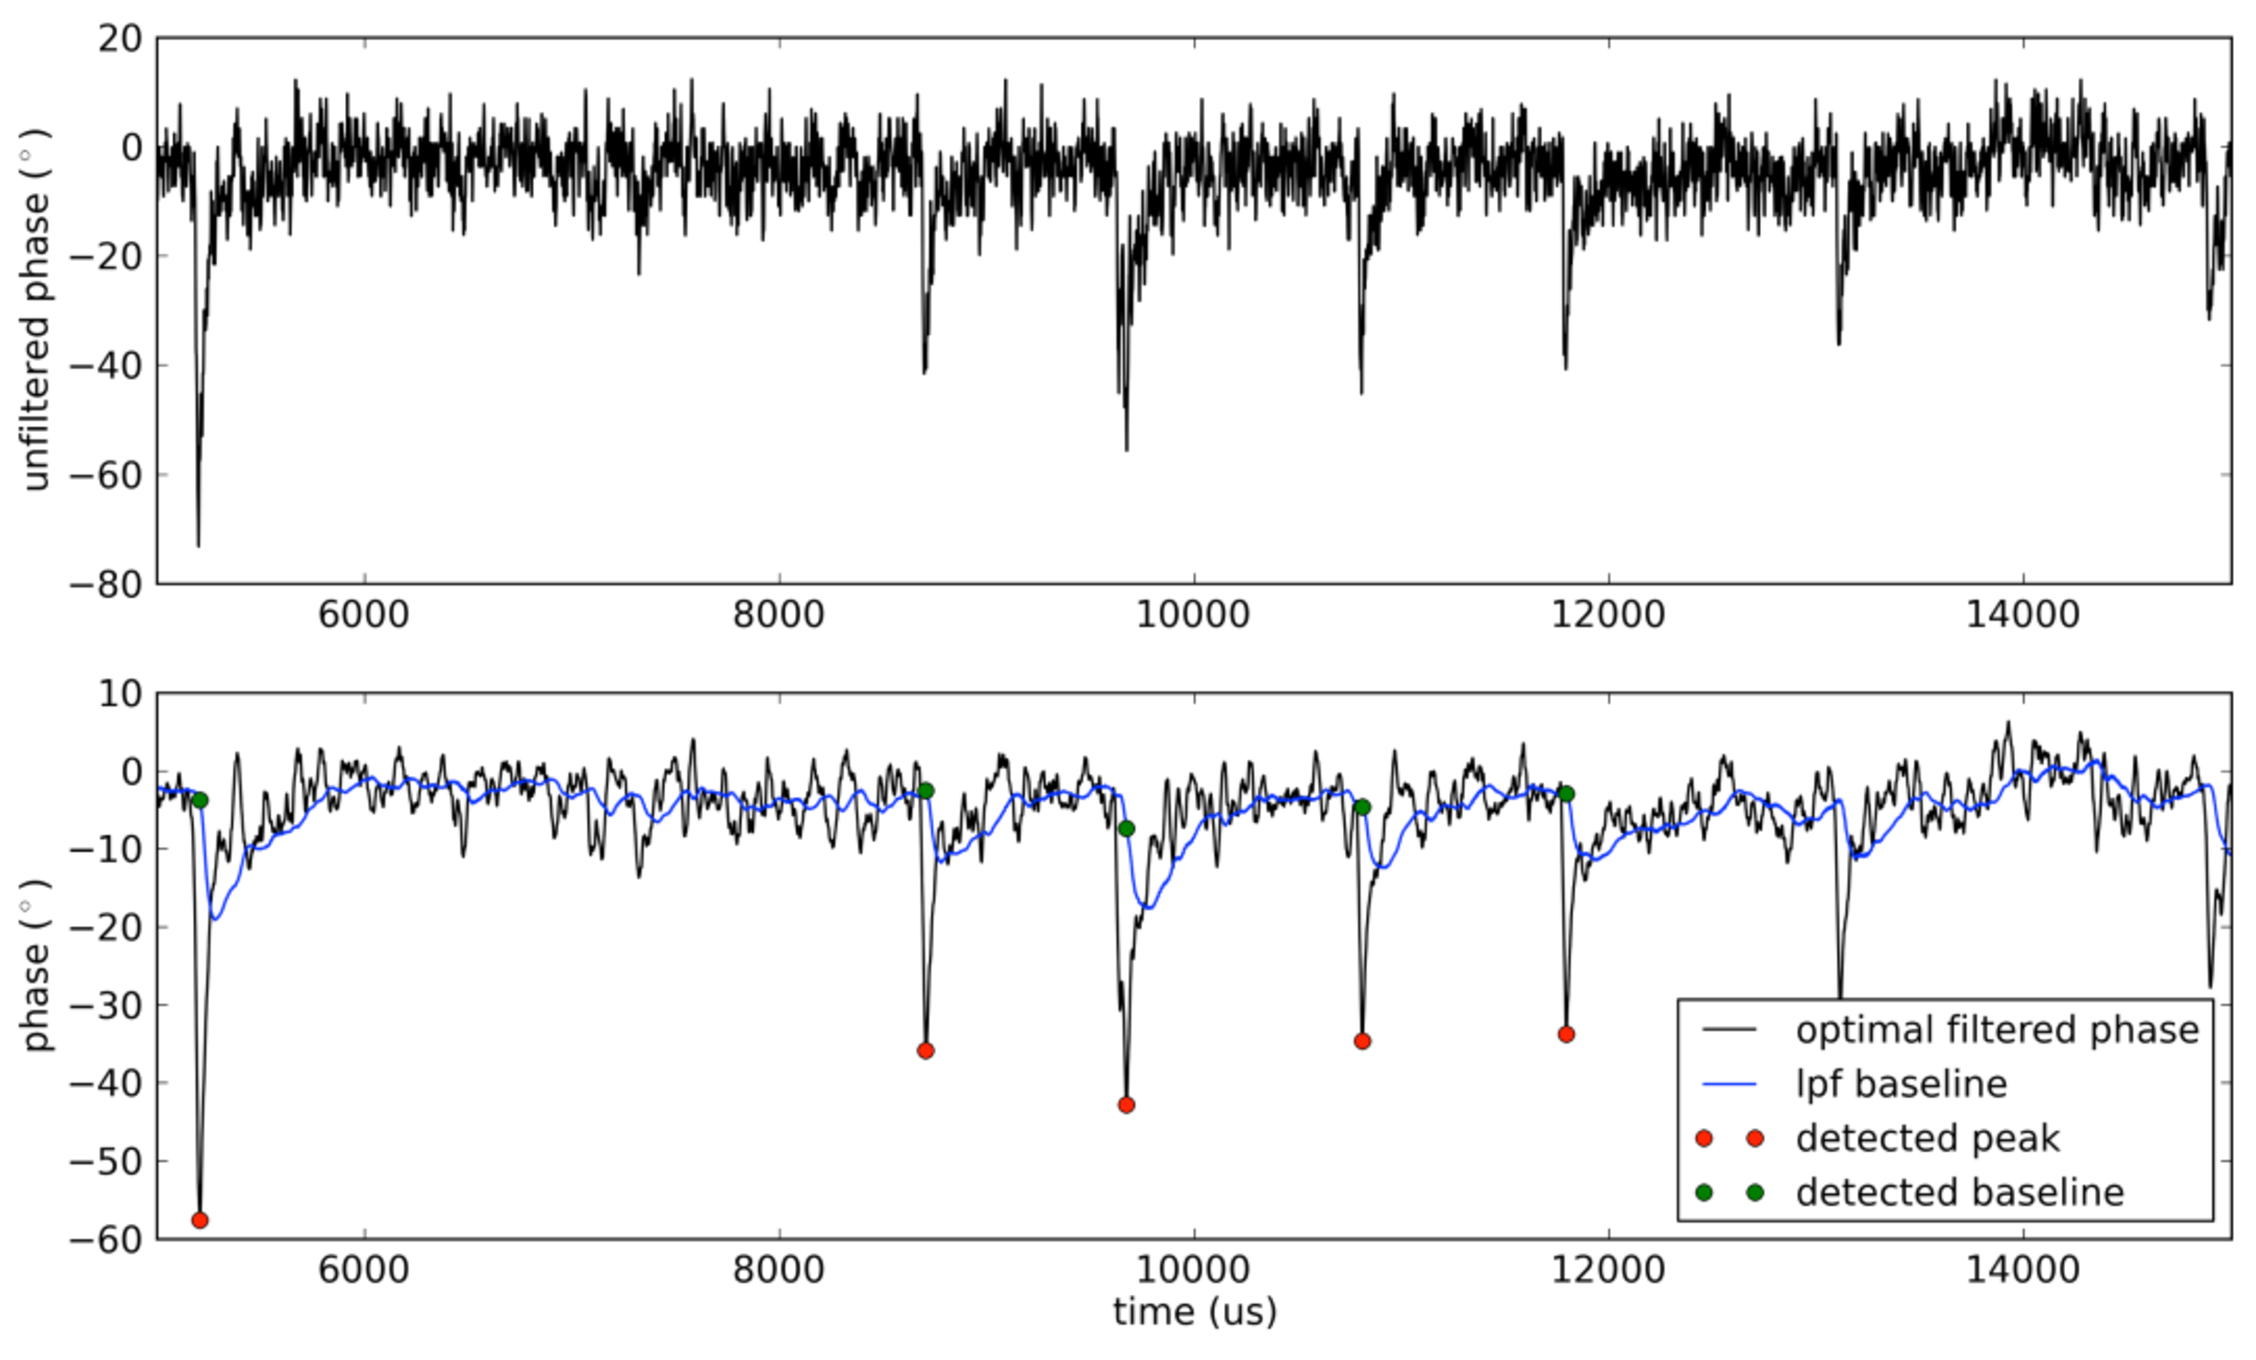
\includegraphics[width=0.98\textwidth]{pulsos_de_fase}
								\end{column}
				\end{columns}
				\scriptsize{A (programmable) filter is applied to the phase signal to increase the
				SNR of drops in phase due to photons.  

				{\color{blue}Snapshots	of raw phase data are used to create a
				\alert{matched filter},	customized to each pixel.}

				The {\color{blue}firmware} also keeps track of the phase baseline and subtracts it
				before checking for photon pulses, to resist false triggers from $1/f$
				noise.\footnote{ARCONS talks.}}
\end{frame}
%\begin{frame}{Readout design and development}
%
%				MKIDs $\to$ 
%
%				The obvious advantage of MKIDs over competing cryogenic technologies
%				like TESs is the elimination of the cryogenic electronics required for
%				multiplexing
%
%				\tiny{\emph{\textbf{A readout for large arrays of microwave kinetic
%				inductance detectors}}, Rev. Sci. Instrum., doi:10.1063/1.3700812}
%\end{frame}

\begin{frame}{Design requirements}
				\begin{itemize}
								\item The readout must not introduce significant noise above the
												system noise floor set by the \textbf{cryogenic
												amplifier} with a noise temperature of $\sim
												4\,\text{K}$.
								\item The entire readout system must be capable of
												reading out at least \alert{512 resonators} in $\sim
												1\,\text{GHz}$ of bandwidth ({\color{red} to be
												confirmed}).
								\item \alert{Crosstalk} between channels greater than
												$250\,\text{kHz}$ apart should be less than \alert{1\%}.
								\item Intrinsic energy resolution \alert{$R \sim 20-150$}
												\footnote{Rev.Sci.Instr. 83, 044702 (2012)}
				\end{itemize}
\end{frame}

\begin{frame}{The cryogenic amplifier}
				%\begin{itemize}
				%\item 
				The double sideband (DSB) phase noise of the HEMT
												amplifier is given by the simple expression, 
												{\color{red}
												\begin{equation}
																N_{\phi \text{DSB}} = \frac{k_B T_n}{P}
												\end{equation}} 
												\flushleft
												$T_n \to$ noise temperature of the amplifier, 

												$P \to$ power on the input. 

												The readout power for each MKID should be $-100 \pm
												15\,\text{dBm}$ ({\color{red} to be confirmed}). 

												For	$-85\,\text{dBm}$ readout power, off resonance, and $T_n
												= 6\,\text{K}$, we expect $-106\,\text{dBc/Hz}$ for the
												HEMT phase noise. Ideally, the readout electronics will
												contribute noise well below this
												value.\footnote{Rev.Sci.Instr. 83, 044702 (2012)}
												%\end{itemize}
\end{frame}

\begin{frame}{$N_\text{channels}$ vs. $P_\text{readout}$}
				\footnotesize{\textbf{Rev.Sci.Instr. 83, 044702 (2012)}}
				\begin{columns}
								\begin{column}{0.45\textwidth}
												\begin{itemize}
																\item \footnotesize{Given an ADC's voltage noise
																				specification, the number of channels
																				{\color{blue}$n$} an ADC can read out at a given power
																				without adding to the HEMT noise can be
																				calculated.}
																\item The contours of Fig. 3 are calculated by
																				scaling the HEMT noise with a
																				channel-dependent factor giving, $k_B
																				T_n /(p_\text{max}^2 P)$.
																\item $p_\text{max} \propto
																				n^{1/2}\,\text{for}\,n >> 1$
																\item Random phase per tone assumed
												\end{itemize}
								\end{column}
								\begin{column}{0.45\textwidth}
												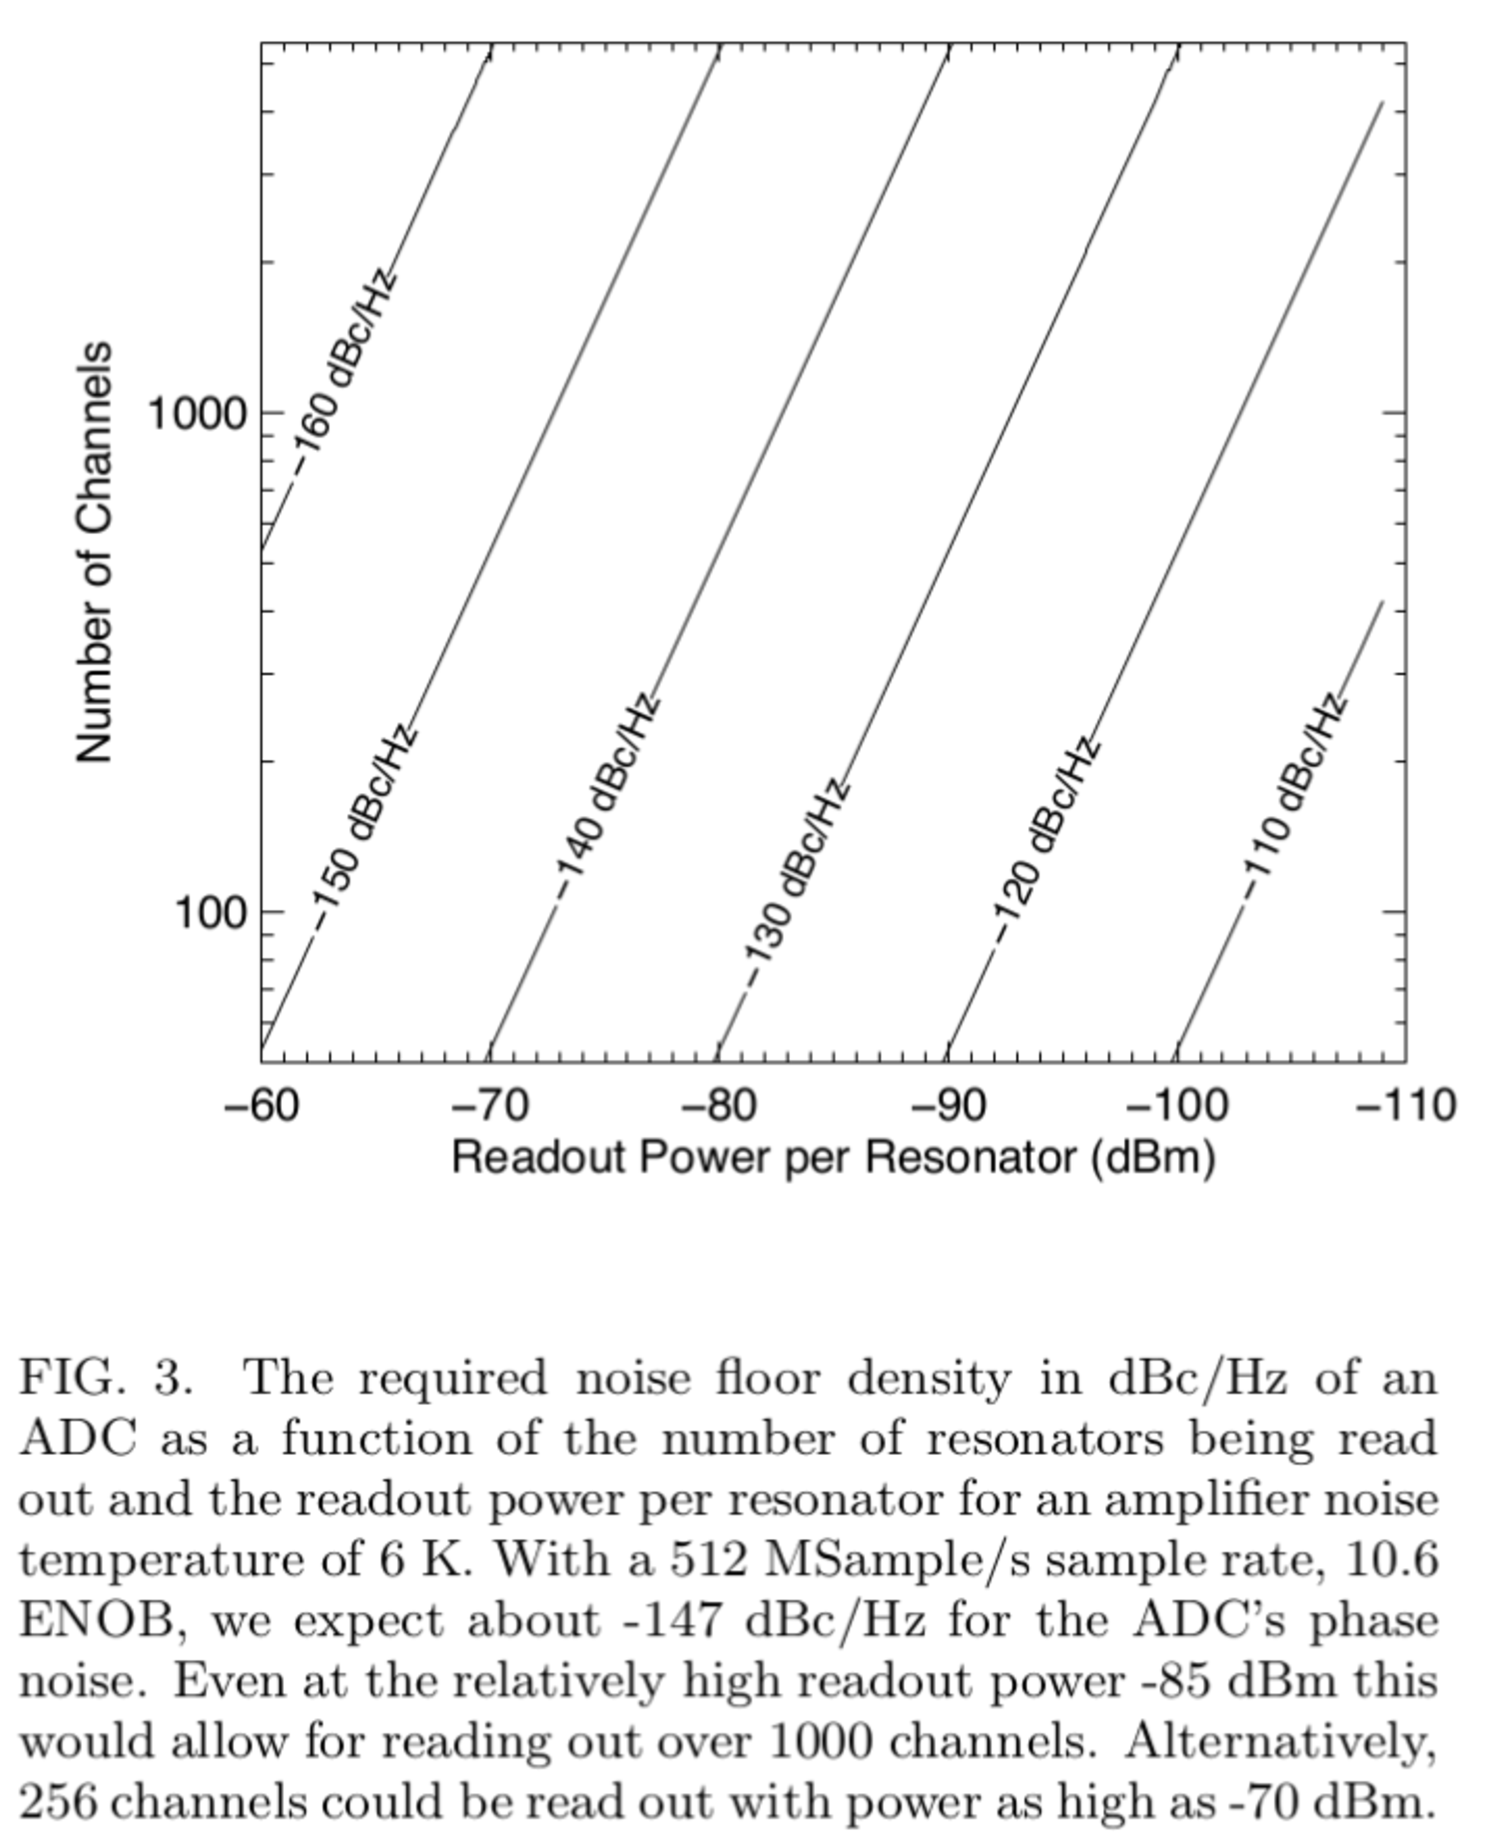
\includegraphics[width=0.85\textwidth]{power_vs_Nchannels}
								\end{column}
				\end{columns}
\end{frame}

%\section{El algoritmo de Goertzel}
\begin{frame}{El algoritmo de Goertzel}
				\begin{itemize}
								\item Finalize performance requirements for firmware 
								\item Finalize performance requirements for Tx and Rx parts 
								\item First tests of RxChannelizer (front-end, mixers, filters,
												DC-block, etc.)
				\end{itemize}
								\centering
								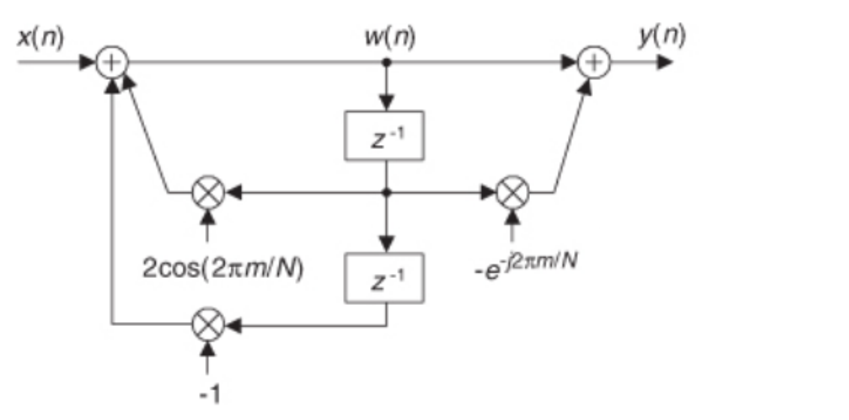
\includegraphics[width=0.45\textwidth]{goertzel_algo}
\end{frame}

\begin{frame}{El algoritmo de Goertzel}
				\begin{itemize}
								\item Finalize performance requirements for firmware 
								\item Finalize performance requirements for Tx and Rx parts 
								\item First tests of RxChannelizer (front-end, mixers, filters,
												DC-block, etc.)
				\end{itemize}
								\centering
								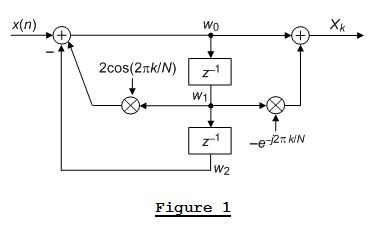
\includegraphics[width=0.45\textwidth]{goertzel_non_integer_figure1}
\end{frame}

\section{Work perspectives}
\begin{frame}{Work perspectives}
				\begin{itemize}
								\item Finalize performance requirements for firmware 
								\item Finalize performance requirements for Tx and Rx parts 
								\item First tests of RxChannelizer (front-end, mixers, filters,
												DC-block, etc.)
				\end{itemize}
\end{frame}
%\section{Prefer titles that make a statement}
%\begin{frame}{Prefer titles that make a statement}
%
%				Many opt for meaningless titles and section titles.  
%
%				Instead, make titles convey information.
%
%				\pause
%
%				Use \texttt{pause} commands almost anywhere to progressively step through material.
%
%				\pause
%
%				\begin{figure}
%								\centering
%								\caption{Figure and table environments also work.
%								Use \texttt{includegraphics} or \texttt{pgfplots}.}
%								\begin{tikzpicture}
%												\begin{axis}[footnotesize,axis lines=middle
%																,xlabel={$t$},no marks,thick,domain=0:2.2,smooth ]
%																\addplot+[]{1-2*exp(-2*x)+exp(-4*x)};
%																\addlegendentry{$u(t)$};
%																\addplot+[]{1-exp(-4*x)};
%																\addlegendentry{$v(t)$};
%																\addplot+[]{1+2*exp(-2*x)+exp(-4*x)};
%																\addlegendentry{$w(t)$};
%												\end{axis}
%								\end{tikzpicture}
%				\end{figure}
%
%\end{frame}
%
%
%
%
%\section{Conclusion}
%\begin{frame}{Conclusion}
%
%				Finish with your conclusions displayed: \emph{not} a list of references, \emph{nor} a meaningless ``thank you'' slide.
%
%				\vfill
%				\begin{quote}
%								Three rules of public speaking: Be forthright.  Be brief.  Be
%								seated. \hfill(S. Dressel \& J. Chew, 1987)
%				\end{quote}
%\end{frame}




\end{document}

